% Aberdeen style guide should be followed when using this
% layout. Their template powerpoint slide is used to extract the
% Aberdeen color and logo but is otherwise ignored (it has little or
% no formatting in it anyway).
%
% http://www.abdn.ac.uk/documents/style-guide.pdf

%%%%%%%%%%%%%%%%%%%% Document Class Settings %%%%%%%%%%%%%%%%%%%%%%%%%
% Pick if you want slides, or draft slides (no animations)
%%%%%%%%%%%%%%%%%%%%%%%%%%%%%%%%%%%%%%%%%%%%%%%%%%%%%%%%%%%%%%%%%%%%%%
%Normal document mode
\documentclass[10pt,compress]{beamer}
%%%%%Draft or handout mode
%\documentclass[10pt,compress,handout]{beamer}
%\documentclass[10pt,compress,handout,ignorenonframetext]{beamer}
\usepackage{comment}
%%%%%%%%%%%%%%%%%%%% General Document settings %%%%%%%%%%%%%%%%%%%%%%%
% These settings must be set for each presentation
%%%%%%%%%%%%%%%%%%%%%%%%%%%%%%%%%%%%%%%%%%%%%%%%%%%%%%%%%%%%%%%%%%%%%%
\newcommand{\shortname}{Dr Jeff Gomes}
\newcommand{\fullname}{Dr Jeff Gomes}
\institute{School of Engineering}
\newcommand{\emailaddress}{jefferson.gomes@abdn.ac.uk}
\newcommand{\logoimage}{../FigBanner/UoAHorizBanner}
\title{Engineering Thermodynamics (EG3521)}
\subtitle{Module 2: Production of Power from Heat}
\date[10-18/02/2014]{10-18 February 2014}

%%%%%%%%%%%%%%%%%%%% Template settings %%%%%%%%%%%%%%%%%%%%%%%%%%%%%%%
% You shouldn't have to change below this line, unless you want to.
%%%%%%%%%%%%%%%%%%%%%%%%%%%%%%%%%%%%%%%%%%%%%%%%%%%%%%%%%%%%%%%%%%%%%%
\usecolortheme{whale}
\useoutertheme{infolines}

% Use the fading effect for items that are covered on the current
% slide.
\beamertemplatetransparentcovered

% We abuse the author command to place all of the slide information on
% the title page.
\author[\shortname]{%
  \fullname\\\ttfamily{\emailaddress}
}


%At the start of every section, put a slide indicating the contents of the current section.
%\AtBeginSection[] {
%  \begin{frame}
%    \frametitle{Section Outline}
%    \tableofcontents[currentsection]
%  \end{frame}
%}

% Allow the inclusion of movies into the Presentation! At present,
% only the Okular program is capable of playing the movies *IN* the
% presentation.
\usepackage{multimedia}
\usepackage{animate}

% \usepackage[usenames,dvipsnames]{pstricks}
% \usepackage{epsfig}
% \usepackage{pst-grad} % For gradients
% \usepackage{pst-plot} % For axes


%%%%% Color settings
\usepackage{color}
%% The background color for code listings (i.e. example programs)
\definecolor{lbcolor}{rgb}{0.9,0.9,0.9}%
\definecolor{UoARed}{rgb}{0.64706, 0.0, 0.12941}
\definecolor{UoALight}{rgb}{0.85, 0.85, 0.85}
\definecolor{UoALighter}{rgb}{0.92, 0.92, 0.92}
\setbeamercolor{structure}{fg=UoARed} % General background and higlight color
\setbeamercolor{frametitle}{bg=black} % General color
\setbeamercolor{frametitle right}{bg=black} % General color
\setbeamercolor{block body}{bg=UoALighter} % For blocks
\setbeamercolor{structure}{bg=UoALight} % For blocks
% Rounded boxes for blocks
\setbeamertemplate{blocks}[rounded]

%%%%% Font settings
% Aberdeen requires the use of Arial in slides. We can use the
% Helvetica font as its widely available like so
% \usepackage{helvet}
% \renewcommand{\familydefault}{\sfdefault}
% But beamer already uses a sans font, so we will stick with that.

% The size of the font used for the code listings.
\newcommand{\goodsize}{\fontsize{6}{7}\selectfont}

% Extra math packages, symbols and colors. If you're using Latex you
% must be using it for formatting the math!
\usepackage{amscd,amssymb} \usepackage{amsfonts}
\usepackage[mathscr]{eucal} \usepackage{mathrsfs}
\usepackage{latexsym} \usepackage{amsmath} \usepackage{bm}
\usepackage{amsthm} \usepackage{textcomp} \usepackage{eurosym}
% This package provides \cancel{a} and \cancelto{a}{b} to "cancel"
% expressions in math.
\usepackage{cancel}

% Get rid of font warnings as modern LaTaX installations have scalable
% fonts
\usepackage{type1cm} 

%\usepackage{enumitem} % continuous numbering throughout enumerate commands

% For exact placement of images/text on the cover page
\usepackage[absolute]{textpos}
\setlength{\TPHorizModule}{1mm}%sets the textpos unit
\setlength{\TPVertModule}{\TPHorizModule} 

% Source code formatting package
\usepackage{listings}%
\lstset{ backgroundcolor=\color{lbcolor}, tabsize=4,
  numberstyle=\tiny, rulecolor=, language=C++, basicstyle=\goodsize,
  upquote=true, aboveskip={1.5\baselineskip}, columns=fixed,
  showstringspaces=false, extendedchars=true, breaklines=false,
  prebreak = \raisebox{0ex}[0ex][0ex]{\ensuremath{\hookleftarrow}},
  frame=single, showtabs=false, showspaces=false,
  showstringspaces=false, identifierstyle=\ttfamily,
  keywordstyle=\color[rgb]{0,0,1},
  commentstyle=\color[rgb]{0.133,0.545,0.133},
  stringstyle=\color[rgb]{0.627,0.126,0.941}}

% Allows the inclusion of other PDF's into the final PDF. Great for
% attaching tutorial sheets etc.
\usepackage{pdfpages}
\setbeamercolor{background canvas}{bg=}  

% Remove foot note horizontal rules, they occupy too much space on the slide
\renewcommand{\footnoterule}{}

% Force the driver to fix the colors on PDF's which include mixed
% colorspaces and transparency.
\pdfpageattr {/Group << /S /Transparency /I true /CS /DeviceRGB>>}

% Include a graphics, reserve space for it but
% show it on the next frame.
% Parameters:
% #1 Which slide you want it on
% #2 Previous slides
% #3 Options to \includegraphics (optional)
% #4 Name of graphic
\newcommand{\reserveandshow}[4]{%
\phantom{\includegraphics<#2|handout:0>[#3]{#4}}%
\includegraphics<#1>[#3]{#4}%
}

\begin{document}

% Title page layout
\begin{frame}
  \titlepage
  \vfill%
  \begin{center}
    \includegraphics[clip,width=0.8\textwidth]{\logoimage}
  \end{center}
\end{frame}

% Table of contents
%\frame{ \frametitle{Slides Outline}
%  \tableofcontents
%}


%%%%%%%%%%%%%%%%%%%% The Presentation Proper %%%%%%%%%%%%%%%%%%%%%%%%%
% Fill below this line with \begin{frame} commands! It's best to
% always add the fragile option incase you're going to use the
% verbatim environment.
%%%%%%%%%%%%%%%%%%%%%%%%%%%%%%%%%%%%%%%%%%%%%%%%%%%%%%%%%%%%%%%%%%%%%%

\section{Module 2.1: Vapour Power Systems}

%%%
%%% Slide
%%%
\subsection{Motivation}
\begin{frame}
 \frametitle{Aims and Objectives}
 At the end of this first set of lecture, you should be able to:
 \begin{enumerate}[(i)]
  \item <2-> Apply the Second Law of Thermodynamics to understand power systems operating with water/steam;
  \item <3-> Identify the engines/equipment commonly found industrial-based thermodynamic cycles; 
  \item <4-> Study the two power cycles relevant to vapour systems: Carnot and Rankine, and; 
  \item <5-> Compare their thermal efficiencies;
  \item <6-> Identify the common operations to improve the cycles' performance / efficiency;
 \end{enumerate}
\end{frame}
 
%%%
%%% Slide
%%%
\subsection{Bibliography} 
\begin{frame}
 \frametitle{Suggested References}
  Literature relevant for this module:
  \begin{enumerate}[(a)]
   \item J.M. Smith, H.C. Van Ness, M.M. Abbott, $\lq$Introduction to Chemical Engineering Thermodynamics', 6$^{th}$ Edition: Chapter 8;
   %\item A.B. Pippard, $\lq$Elements of Classical Thermodynamics' (1966): Chapters 2, 3 and 4;
   \item H. Devoe, $\lq$Thermodynamics and Chemistry', 2$^{nd}$ Edition: Chapter 4;
   \item I. Muller, W.H. Muller, $\lq$Fundamentals of Thermodynamics and Applications', Chapter 6;
   \item \href{http://www.learnthermo.com}{http://www.learnthermo.com}, Chapter 9;
   \item \textcolor{red}{M.J. Moran, H.N. Saphiro, D.D. Boettner, M.B. Bailey, $\lq$Principles of Engineering Thermodynamics', 6$^{th}$ Edition: Chapter 8}.
  \end{enumerate}
\end{frame}


\subsection{Introduction}
%%%
%%% Slide
%%%
\begin{frame}
 \frametitle{Introduction to Vapour and Gas Power}
 \begin{block}{} 
  \begin{itemize}
   \item <1-> In the last lecture (and also in EG2004 and EG3020) we reviewed the fundamentals and the four Laws of Thermodynamics;
   \item <2-> In this Module we will extend the First and Second Laws to thermal-based cycles applications; 
   \item <3-> We will also discuss the set of equipment used to generate mechanical power from heat;
   %\item <4-> Module II focuses on power cycles whereas in Module III we will discuss refrigeration cycles and heat pumps.
  \end{itemize}
 \end{block}  
\end{frame}


%%%
%%% Slide
%%%
\begin{frame}
 \frametitle{Introduction to Vapour and Gas Power}
    \begin{figure}%
     \begin{center}
      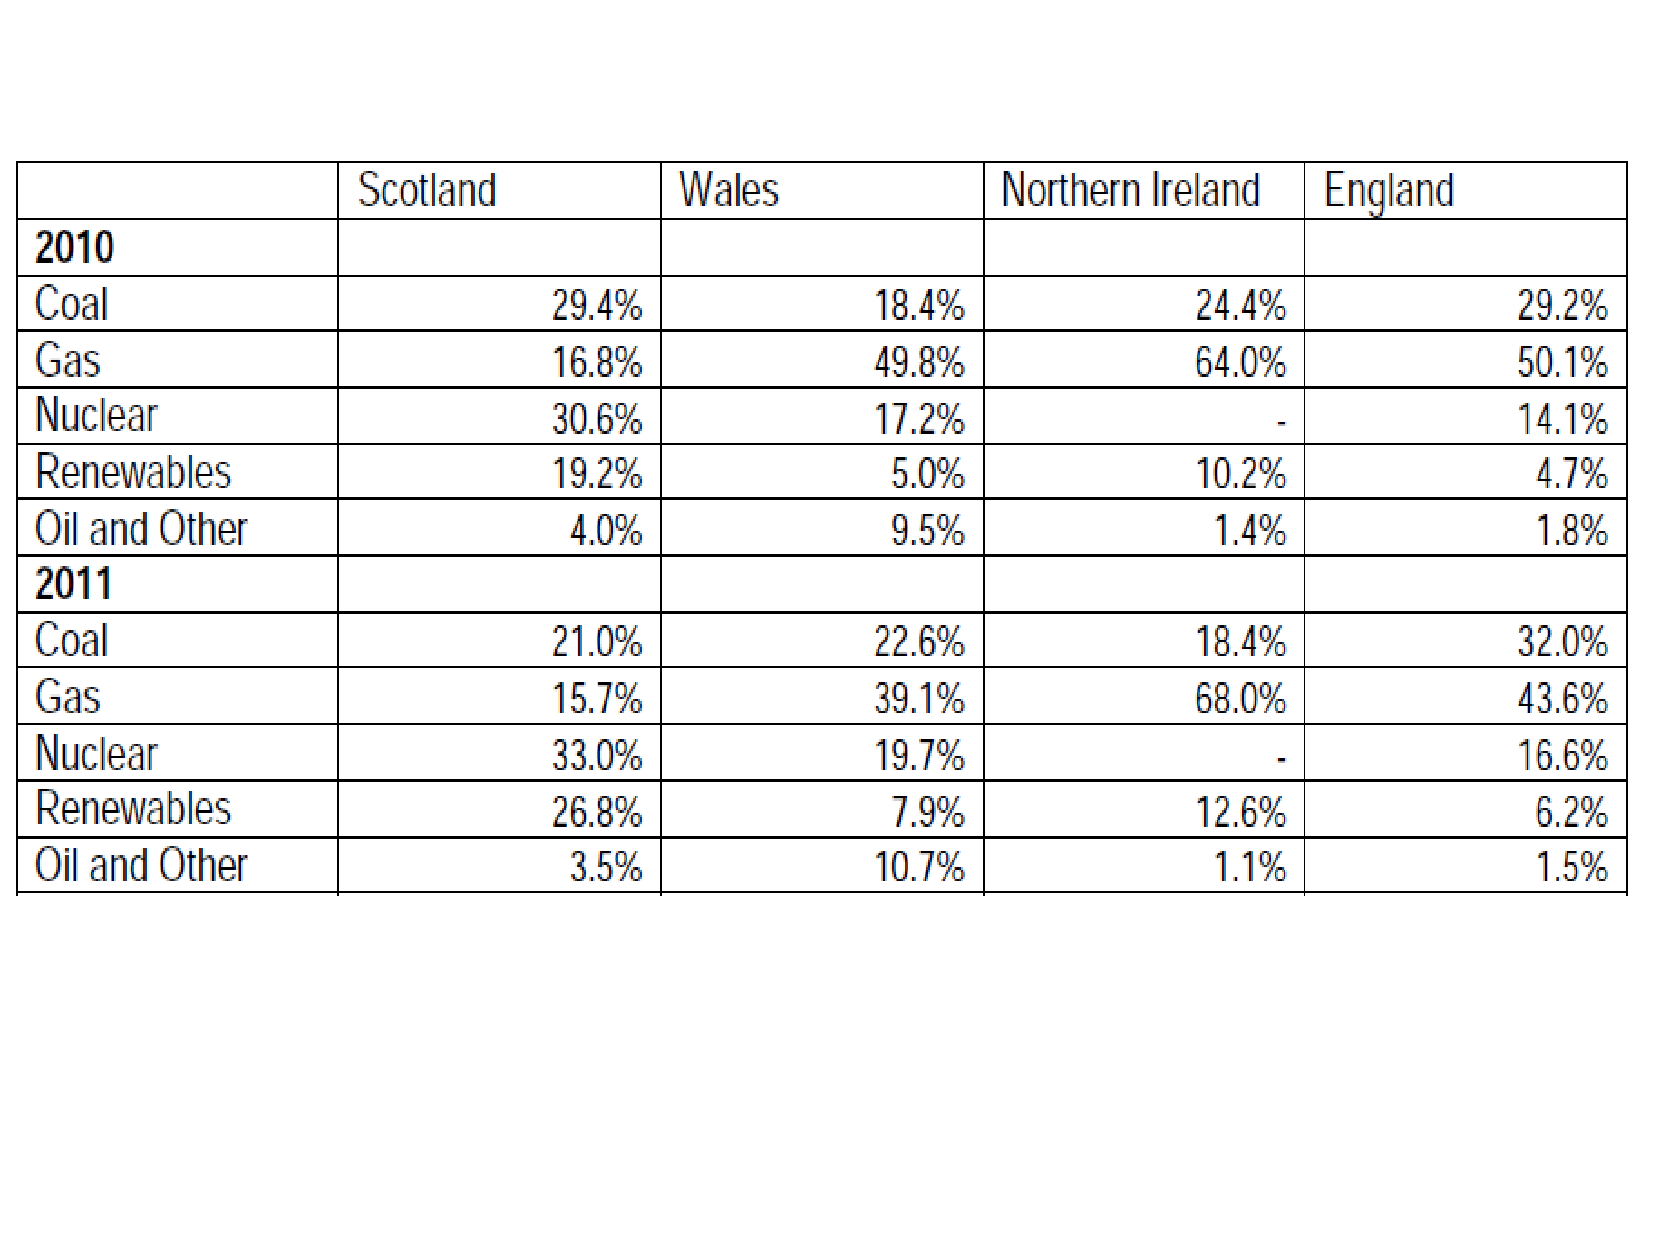
\includegraphics[width=9.cm,clip]{./Pics/Energy_Share_UK}
     \end{center}
    \end{figure}
\vspace{-2cm}
%\scriptsize
\textcolor{blue}{Fuel used in electricity generation and electricity supplied. (\href{https://www.gov.uk/government/organisations/department-of-energy-climate-change/series/electricity-statistics}{https://www.gov.uk/government/organisations/department-of-energy-climate-change/series/electricity-statistics})}
 \normalsize
\end{frame}


%%%
%%% Slide
%%%
\begin{frame}
 \frametitle{Introduction to Vapour and Gas Power}

    \begin{center}
     \begin{table}
       \begin{tabular}{l c c c}
    \hline
    \textcolor{blue}{Power Plant} & \textcolor{blue}{Renewable}  & \textcolor{blue}{Thermodynamic} \\
    \textcolor{blue}{Type}        & \textcolor{blue}{Source}     & \textcolor{blue}{Cycle}         \\
    \hline
      Coal                        &   No                         & Rankine  \\
      Natural Gas                 &   No                         & Brayton  \\
      Nuclear                     &   No                         & Rankine  \\
      Oil                         &   No                         & Rankine  \\
      Biomass                     &   Yes                        & Rankine  \\
      Geothermal                  &   Yes                        & Rankine  \\
      Solar                       &   Yes                        & Rankine  \\
      Hydroelectric               &   Yes                        & None     \\
      Wind                        &   Yes                        & None     \\
      Currents, tides and         &   Yes                        & None     \\
      waves                       &                              &          \\
    %\hline
    %\hline
      \end{tabular}
     \end{table}
    \end{center}
\end{frame}

%%%
%%% Slide
%%%
\begin{frame}
 \frametitle{Introduction to Vapour and Gas Power}
 %\scriptsize

    \begin{itemize}%\scriptsize
     \item <1-> While coal, natural gas, and nuclear still play important roles as energy sources, contributions from wind power, solar power, and other renewable sources are expected to be increasingly significant up to 2050;
     \item <2-> This table shows that thermodynamic cycles are crucial for a number of power plant types that employ renewable and non-renewable sources;
     \item <3-> The basic building block of vapour power systems is the \textcolor{blue}{Rankine cycle};
     \item <4-> In fossil-fueled plants, the energy required for vaporisation originates in combustion of the fuel (i.e., coal, gas and oil) or fission of nuclear material;  
    \end{itemize}
 \normalsize
\end{frame}

%%%
%%% Slide
%%%
\begin{frame}
 \frametitle{Introduction to Vapour and Gas Power}
 %\scriptsize
Energy sources based on thermal-cycles (YouTube videos):
    \begin{itemize}%\scriptsize
     \item \href{http://www.youtube.com/watch?v=_UwexvaCMWA}{\textcolor{blue}{Nuclear Power Plants (NPP)}};
     \item \href{http://www.youtube.com/watch?v=0mjT8ETB128}{\textcolor{blue}{Coal-Fired Stations}};
     \item \href{http://www.youtube.com/watch?v=oi1TRbiE_Kw}{\textcolor{blue}{Gas Turbine Combined Cycle Power Plant}}.
    \end{itemize}
 \normalsize
\end{frame}

%%%
%%% Slide
%%%
\begin{frame}
 \frametitle{A Few Definitions}
 %%\scriptsize
 \begin{itemize}
  \item <1-> A \textcolor{blue}{cycle} is defined as a repeated series of operations occurring in a certain order. A system is said to have undergone a cycle if it returns to its initial state at the end of the process.  Cycles can be classified as ideal (where there is no heat losses) and real. 
  \item <2-> In \textcolor{blue}{gas cycles}, the working fluid remains in the gas phase throughout the cycle (e.g., air).
  \item <3-> In \textcolor{blue}{vapour cycles}, the working fluid exists as a vapour for part of the cycle and a liquid for the other part -- i.e., the working fluid is alternately vaporised and condensed.
  \item <4-> Steam is the most common working fluid in vapour power cycles as it has many desirable characteristics: low cost, availability and high enthalpy of vaporisation.
  \item <5-> Coal, nuclear and natural gas power plants are examples of steam power plants. Each utilises a different type of fuel to supply heat to the steam cycle. 
  \item <6-> In \textcolor{blue}{closed cycles}, after each pass through the cycle the working fluid remains within the system.
  \item <7-> In \textcolor{blue}{open cycles}, after a few (or a single) pass through the cycle the working fluid is replaced by a fresh working fluid.
 \end{itemize}
 %\normalsize
\end{frame}


%%%
%%% Slide
%%%
\begin{frame}
 \frametitle{A Few Definitions -- Open Cycles}
 %\scriptsize
 \begin{columns}
  \begin{column}[c]{0.4\linewidth}
   \begin{itemize}
    \item After compression, air and fuel enters a combustion chamber and the combustion products (e.g., water vapour, CO$_{2}$, CO, N$_{2}$, NO$_{x}$ etc) expand, drive the turbine and are discharged;
   \end{itemize}
  \end{column}
  \begin{column}[c]{0.6\linewidth}
   \begin{figure}%
    \begin{center}
     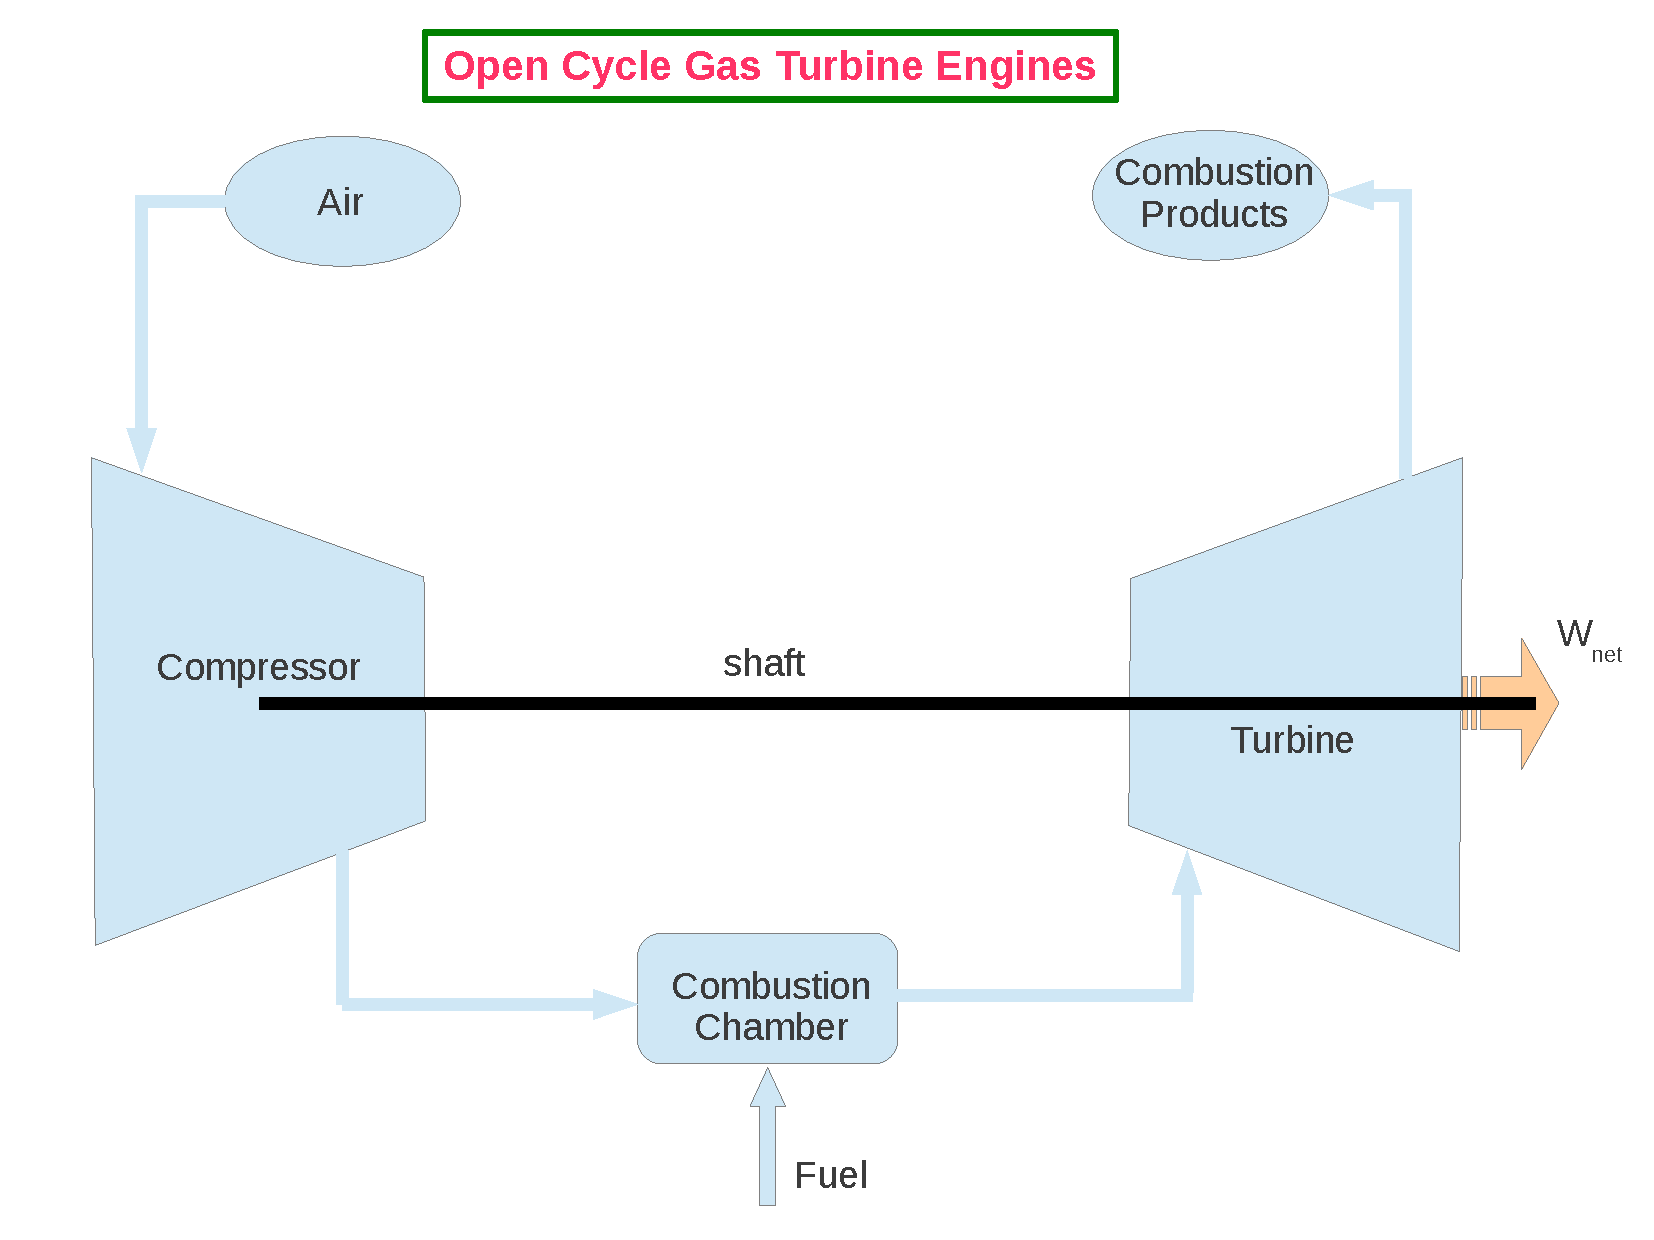
\includegraphics[width=7.5cm,clip]{./Pics/Open_Gas_Turbine_Engines}
    \end{center}
   \end{figure}  
  \end{column}  
 \end{columns}
 \normalsize

\end{frame}


%%%
%%% Slide
%%%
\begin{frame}
 \frametitle{A Few Definitions -- Open Cycles}
 %\scriptsize
 \begin{columns}
  \begin{column}[c]{0.4\linewidth}
   \begin{itemize}
    \item Various processes are involved:
     \begin{enumerate}[(i)]
     %\scriptsize
      \item <2-> Isentropic (reversible adiabatic) compression;
      \item <3-> Constant pressure heat supply in the combustion chamber;
      \item <4-> Isentropic (reversible adiabatic) expansion of combustion gases;
      \item <5-> combustion products are exhausted into the atmosphere.
     \end{enumerate}
   \end{itemize}
  \end{column}
  \begin{column}[c]{0.6\linewidth}
   \begin{figure}%
    \begin{center}
     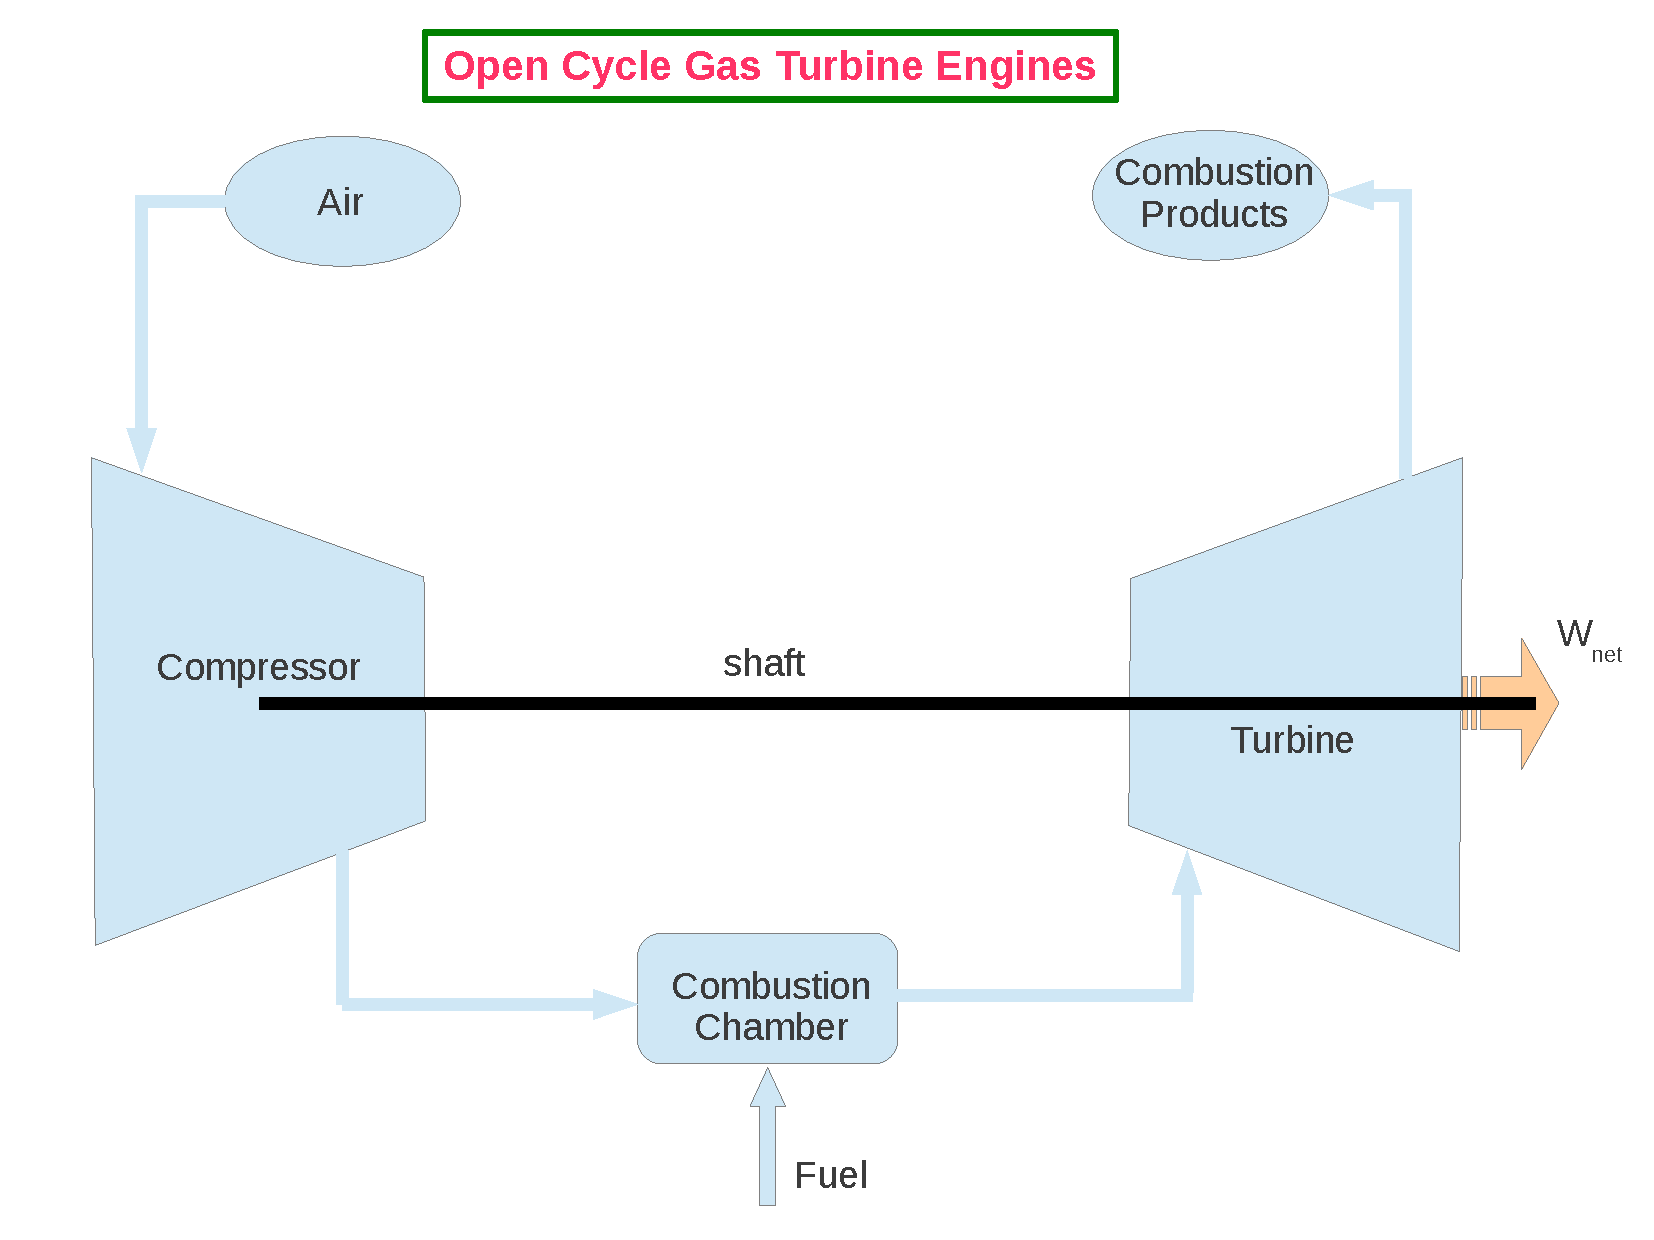
\includegraphics[width=7.5cm,clip]{./Pics/Open_Gas_Turbine_Engines}
    \end{center}
   \end{figure}  
  \end{column}  
 \end{columns}
 \normalsize

\end{frame}



%%%
%%% Slide
%%%
\begin{frame}
 \frametitle{A Few Definitions -- Closed Cycles}
 %\scriptsize
 \begin{columns}
  \begin{column}[c]{0.4\linewidth}
   \begin{itemize}
    \item <1-> It comprises a compressor, air heater, turbine and a cooler;
    \item <2-> Fuel is burnt externally and heat is supplied to working substance (fluid) in heater;
    \item <3-> It uses an external combustion turbine;
   \end{itemize}
  \end{column}
  \begin{column}[c]{0.6\linewidth}
   \begin{figure}%
    \begin{center}
     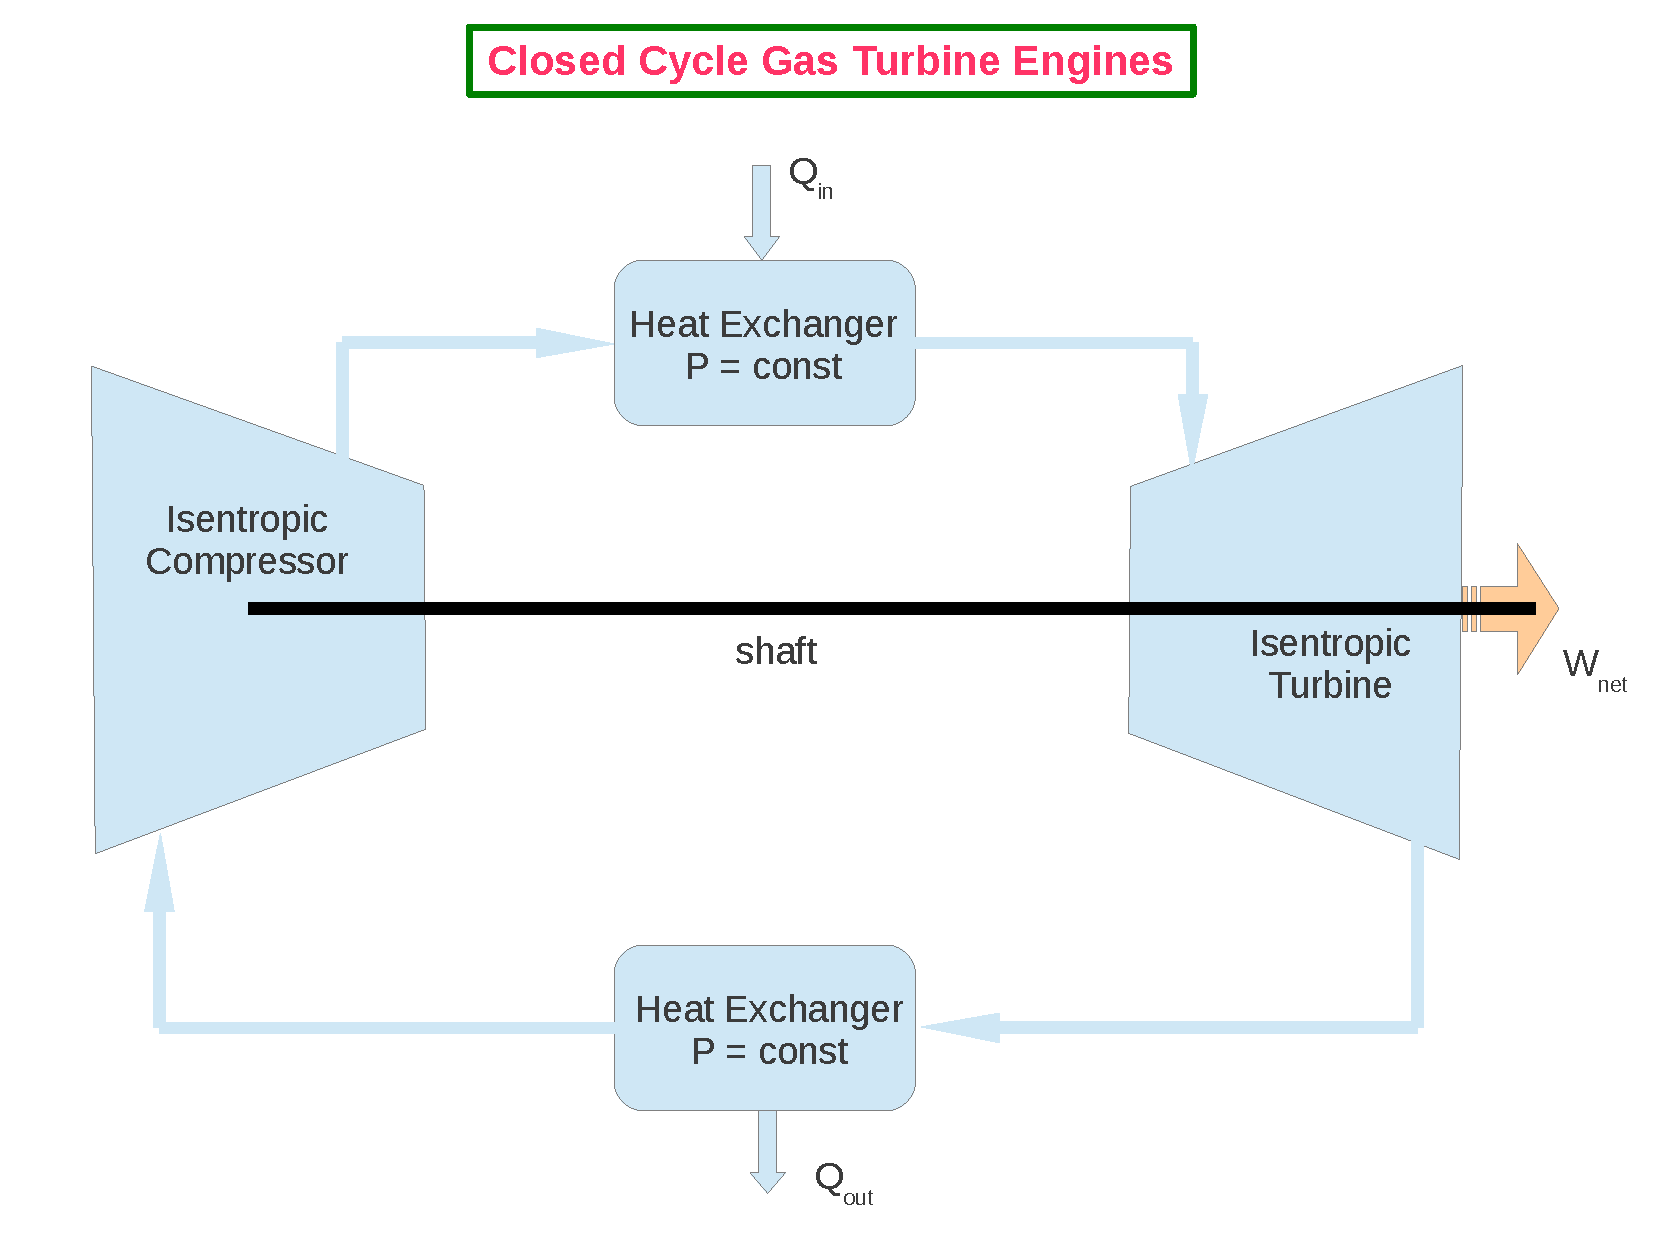
\includegraphics[width=7.5cm,clip]{./Pics/Closed_Gas_Turbine_Engines}
    \end{center}
   \end{figure}  
  \end{column}  
 \end{columns}

 \normalsize

\end{frame}


%%%
%%% Slide
%%%
\begin{frame}
 \frametitle{A Few Definitions -- Open and Closed Cycles}
 %\scriptsize
   \begin{itemize}
    \item <1-> External combustion plants $\Longrightarrow$ wide range of fuel can be used in closed cycles; 
    \item <2-> In open cycles only air can be used as a working fluid;
    \item <3-> Closed cycles requires external furnaces for combustion processes -- the cycle is therefore more complex and costly.
   \end{itemize}

 \normalsize

\end{frame}



\subsection{Carnot Engines and Carnot Cycle}

%%%
%%% Slide
%%%
\begin{frame}
 %\scriptsize
 \frametitle{The Carnot Cycle}
  \begin{columns}
   \begin{column}[c]{0.5\linewidth}
    \begin{itemize} 
     \item <1-> A heat engine is a closed system that converts heat to work and operates in a cycle;
     \item <2-> A Carnot cycle has four reversible steps, alternating isothermal (and constant pressure: 4-1, 2-3) and frictionless adiabatic (1-2, 3-4):
    \end{itemize} 

   \end{column}
   \begin{column}[c]{0.5\linewidth}
   \begin{figure}%
    \begin{center}
     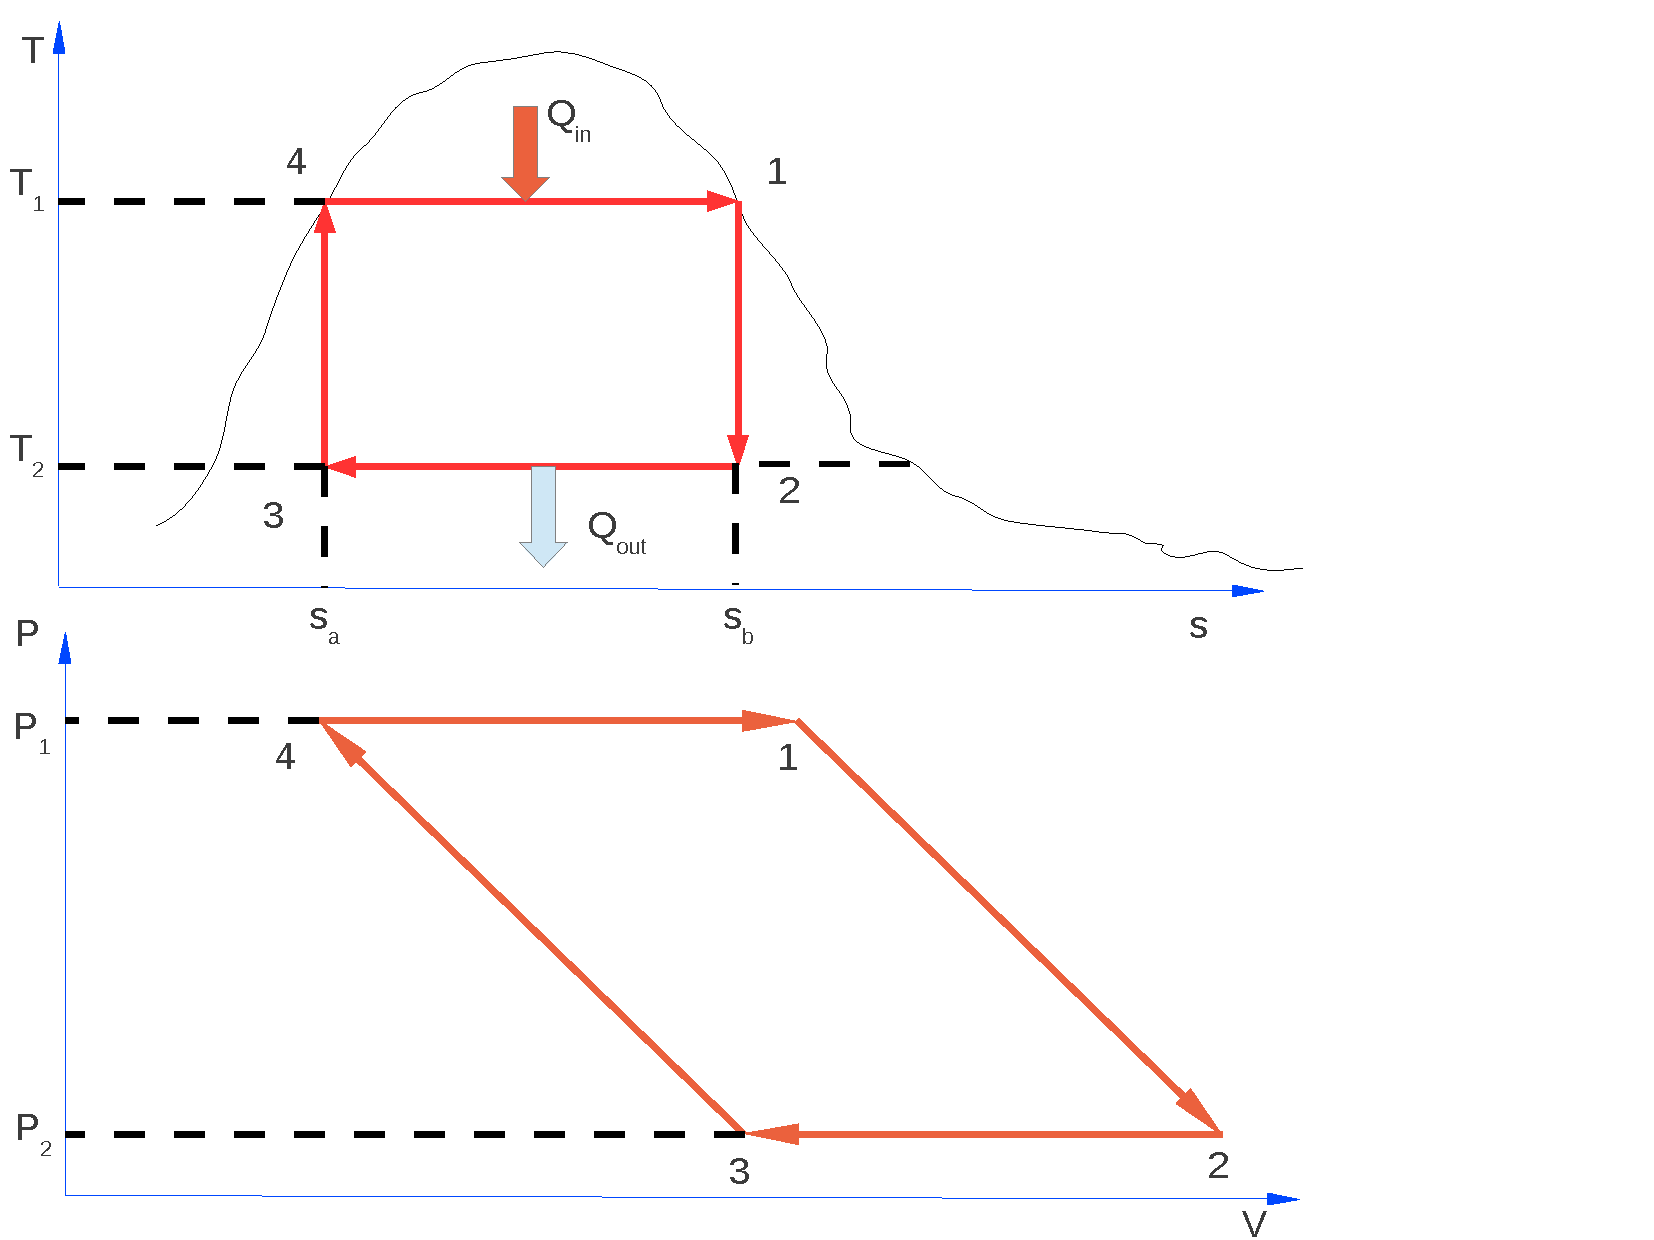
\includegraphics[width=8.cm,clip]{./Pics/Carnot_PV_TS}
    \end{center}
   \end{figure}    

   \end{column}
  \end{columns}
 \normalsize
\end{frame}



%%%
%%% Slide
%%%
\begin{frame}
 %\scriptsize
 \frametitle{The Carnot Cycle}
  \begin{columns}
   \begin{column}[c]{0.5\linewidth}
     \begin{enumerate}[(a)]
     %\scriptsize
      \item <1-> {\it Step 4-1}: 1 kg of boiling water at temperature $T_{1}$ is heated to form wet steam $\left(\right.$dryness fraction $x_{1}\left.\right)$. Heat is then absorbed at constant temperature $\left(T_{1}\right)$ and pressure $\left(P_{1}\right)$;
      \item <2-> {\it Step 1-2}: Steam is isentropically expanded to $T_{2}$ and $P_{2}$;
      \item <3-> {\it Step 2-3}: Heat is rejected at constant pressure $\left(P_{2}\right)$ and temperature $\left(T_{2}\right)$. During this step, steam becomes wetter and cooled;
      \item <4-> {\it Step 3-4}: Wet steam is isentropically compressed until the steam returns to its original state at $T_{1}$ and $P_{1}$.
     \end{enumerate}

   \end{column}
   \begin{column}[c]{0.5\linewidth}
   \begin{figure}%
    \begin{center}
     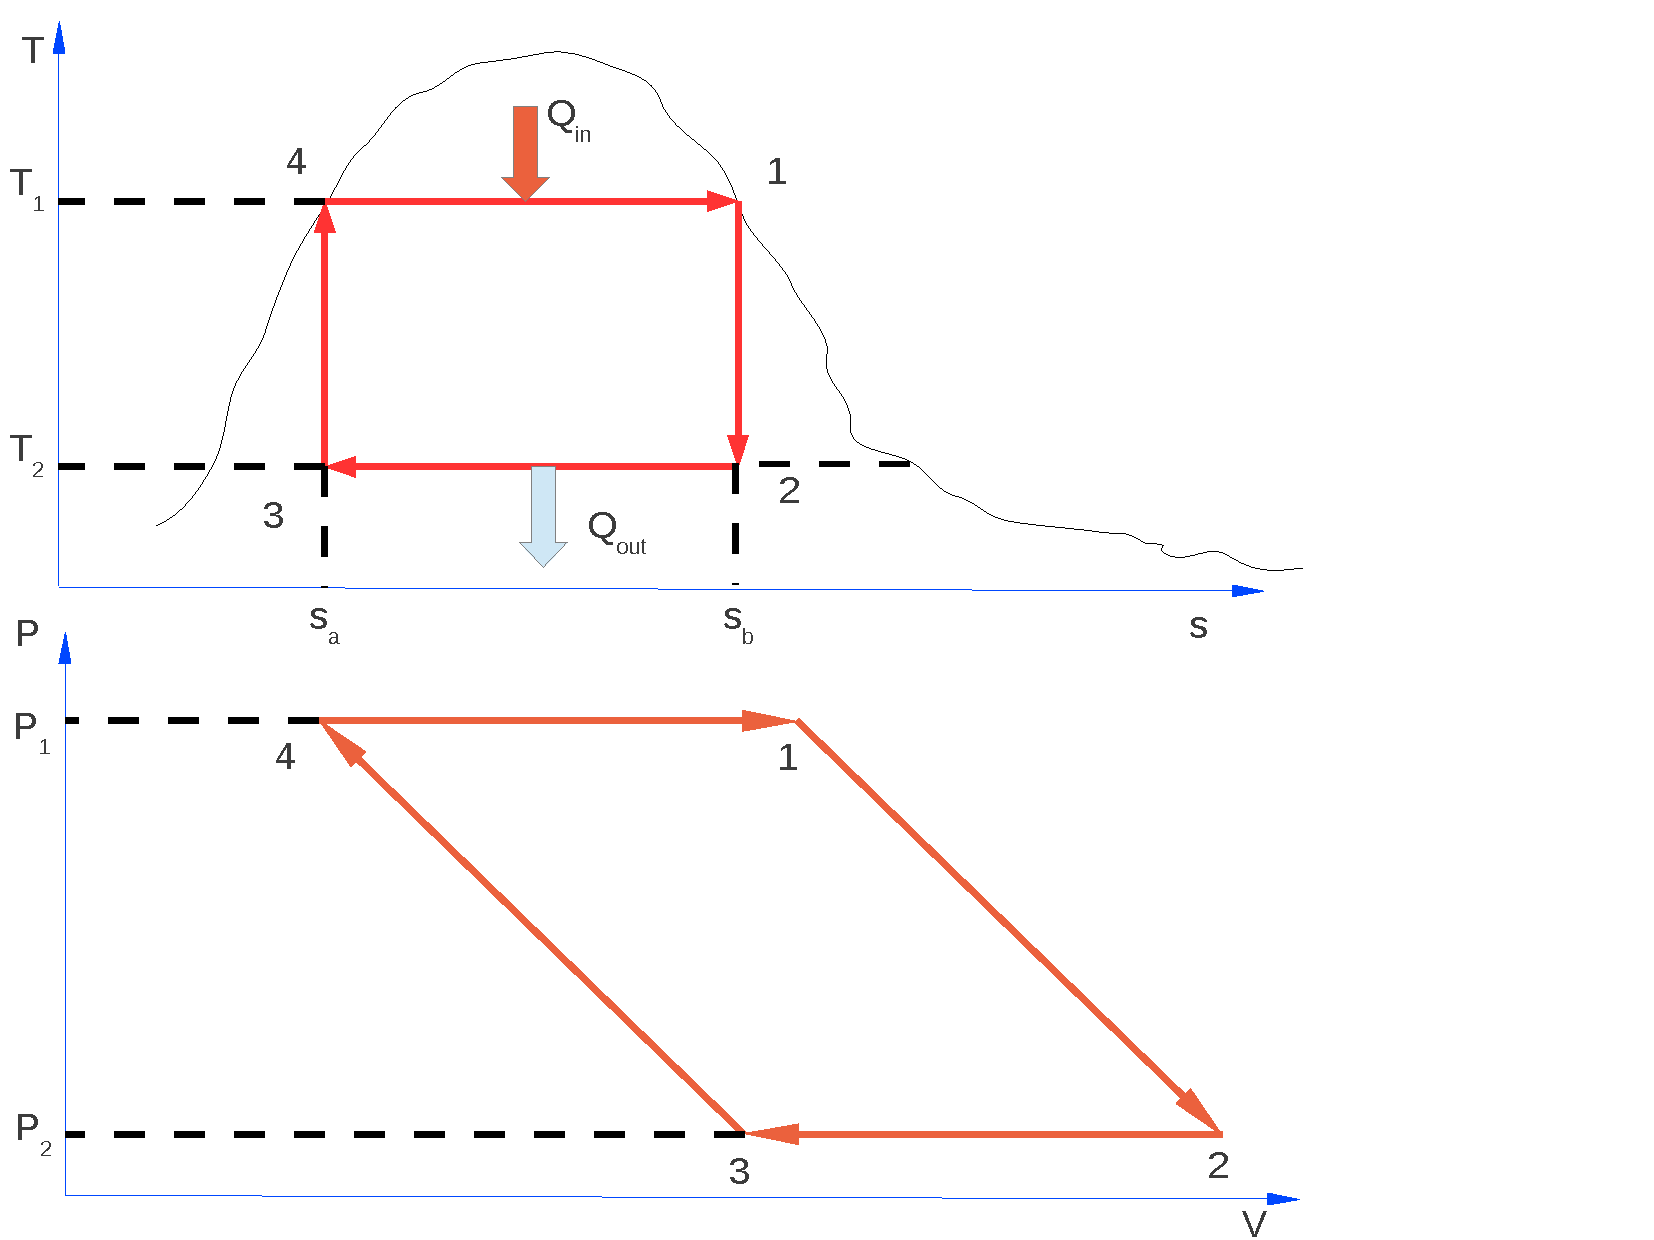
\includegraphics[width=8.cm,clip]{./Pics/Carnot_PV_TS}
    \end{center}
   \end{figure}    

   \end{column}
  \end{columns}
 \normalsize
\end{frame}



%%%
%%% Slide
%%%
\begin{frame}
 %\scriptsize
 \frametitle{The Carnot Cycle}
  \begin{columns}
   \begin{column}[c]{0.5\linewidth}
     \begin{itemize}
      \item <1-> $Q_{4}^{1}\left(T_{1}\right) = \text{Area}\left[ 4-1-s_{a}-s_{b}\right] = T_{1}\left(s_{1}-s_{4}\right) = T_{1}\left(s_{2}-s_{3}\right)$;
\medskip
      \item <2-> $Q_{2}^{3}\left(T_{2}\right) = \text{Area}\left[2-3-s_{a}-s_{b}\right] = T_{2}\left(s_{2}-s_{3}\right)$.
    \end{itemize} 

   \end{column}
   \begin{column}[c]{0.5\linewidth}
   \begin{figure}%
    \begin{center}
     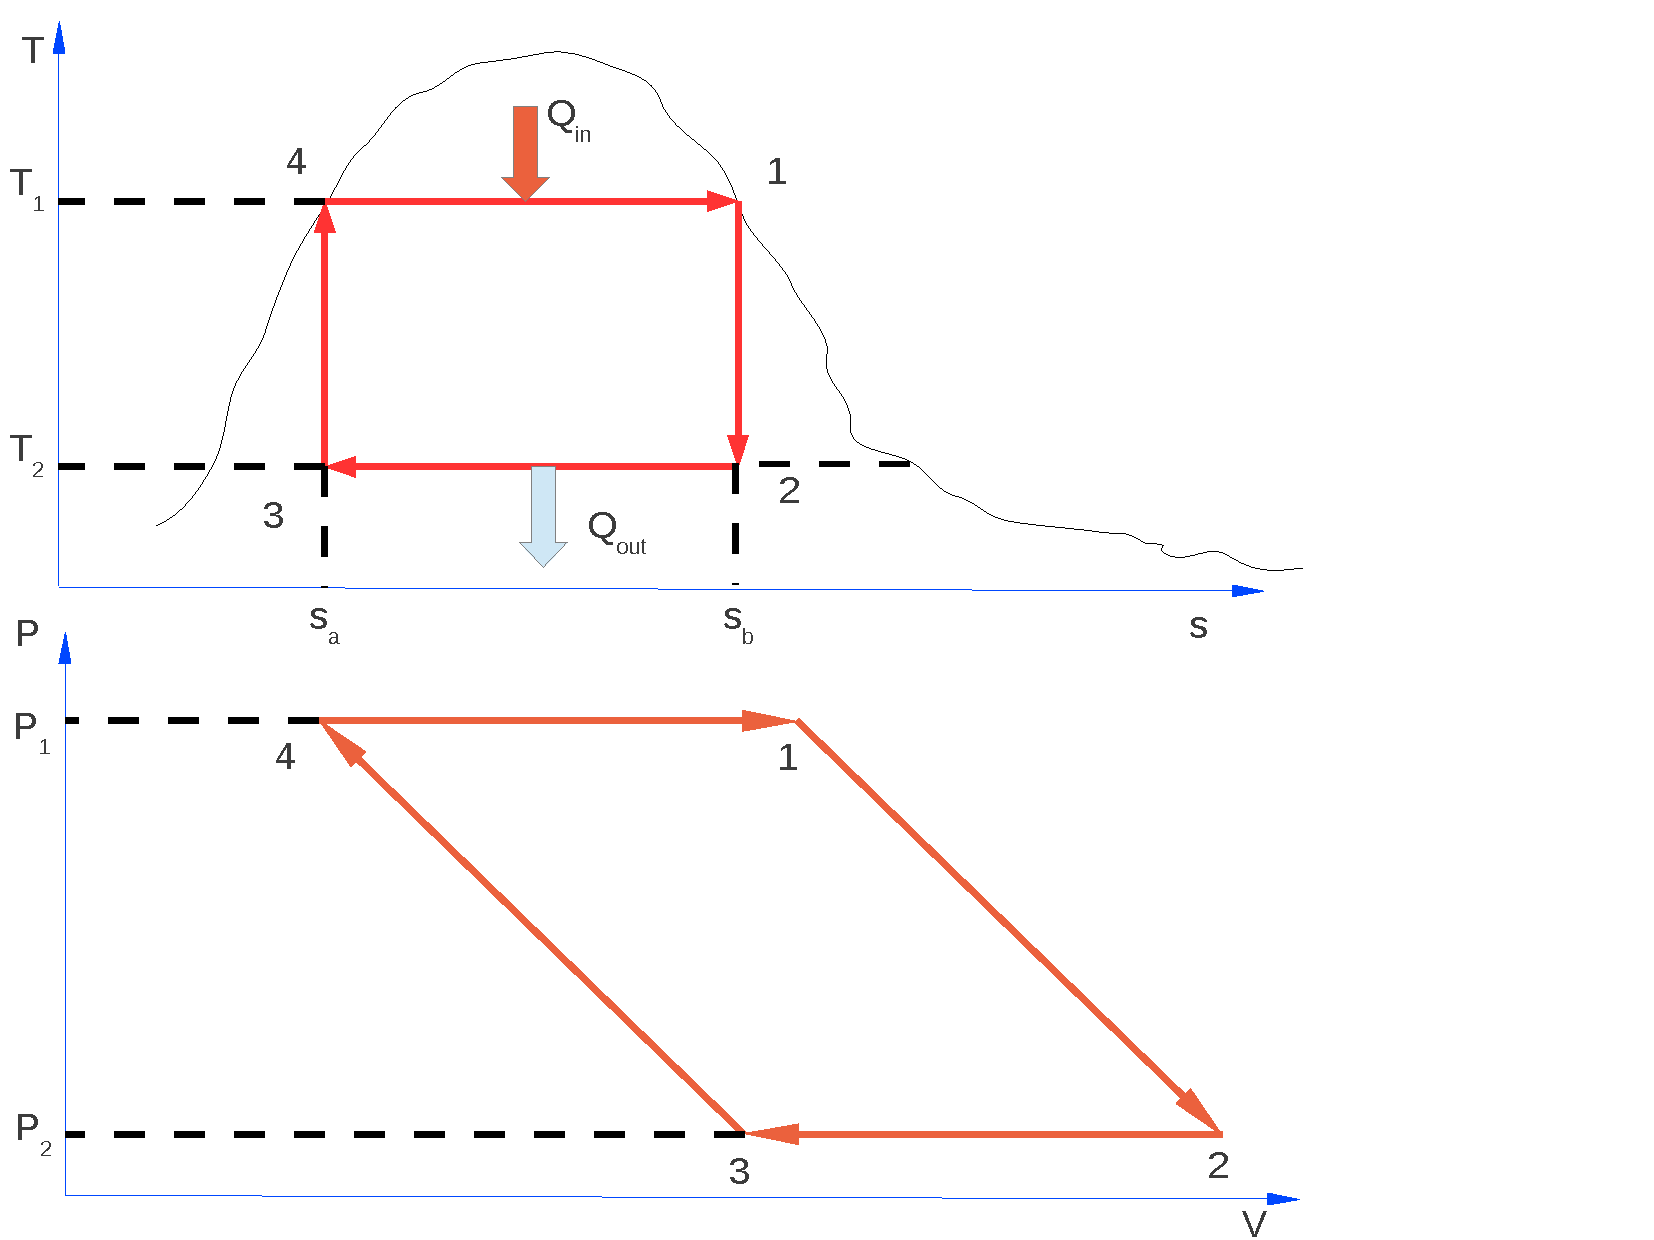
\includegraphics[width=8.cm,clip]{./Pics/Carnot_PV_TS}
    \end{center}
   \end{figure}    

   \end{column}
  \end{columns}
 \normalsize
\end{frame}



%%%
%%% Slide
%%%
\begin{frame}
 %\scriptsize
 \frametitle{The Carnot Cycle}
    \begin{itemize} 
     \item <1-> As there is no heat exchange during isentropic operation (1-2) and (3-4): 
     \item <2-> \textcolor{blue}{Net Work Done = Heat Supplied - Heat Rejected}
      \begin{eqnarray}
       \text{Net Work Done} &=& T_{1}\left(s_{2}-s_{3}\right)-T_{2}\left(s_{2}-s_{3}\right) \nonumber \\
                            &=& \left(T_{1}-T_{2}\right)\left(s_{2}-s_{3}\right)\nonumber
      \end{eqnarray}
     \item <3-> And the Carnot cycle efficiency:\\
      \begin{eqnarray}
        \eta &=& \displaystyle\frac{\text{Work Done}}{\text{Heat Supplied}} \nonumber \\
             &=& \displaystyle\frac{\left(T_{1}-T_{2}\right)\left(s_{2}-s_{3}\right)}{T_{1}\left(s_{2}-s_{3}\right)} \nonumber \\
             & & \nonumber \\
        \textcolor{red}{\eta} &=& \displaystyle\frac{\left(T_{1}-T_{2}\right)}{T_{1}} = \textcolor{red}{1 - \displaystyle\frac{T_{2}}{T_{1}}} \nonumber
      \end{eqnarray}
    \end{itemize}
\end{frame}


%%%
%%% Slide
%%%
\begin{frame}
 \frametitle{Limitations of the Carnot Cycle}
 %\scriptsize
 \begin{enumerate}
  \item <1-> Carnot cycle is thermodynamically simple and has the \textcolor{red}{highest thermal efficiency} for a given temperature gradient;
  \item <2-> It is however {\it difficult to operate in practice} due to:
  \begin{itemize}
  %\scriptsize
   \item <3-> It is difficult to compress a wet vapour isentropically to the saturated state (as required by the process 3-4);
   \item <4-> It is difficult to control the quality of the condensate produced by the condenser to reach state 3;
   \item <5-> The efficiency is greatly affected by $T_{1}$ at which heat is transferred to the working fluid. As the critical temperature of steam is 374 $^{o}C$ therefore, if the cycle is to be operated in the wet region, the maximum possible temperature is severely limited;
   \item <6-> The cycle is even more difficult to operate in practice with superheated steam due to the necessity to supply superheated steam at constant temperature instead of constant pressure (as it is usual in industrial plants);
   \item <7-> \textcolor{blue}{{\it In a practical cycle, limits of pressure and volume are easier to be obtained than limits of temperature. Therefore no practical engine operates in the Carnot cycle, although all modern cycles aspire to achieve it.}}
  \end{itemize}
 \end{enumerate}
 \normalsize
\end{frame}



\subsection{The Rankine Cycle}

%%%
%%% Slide
%%%
\begin{frame}
 \frametitle{Rankine Cycle}
 %\scriptsize
 \begin{columns}
   \begin{column}[c]{0.6\linewidth}
    \begin{figure}%
     \begin{center}
      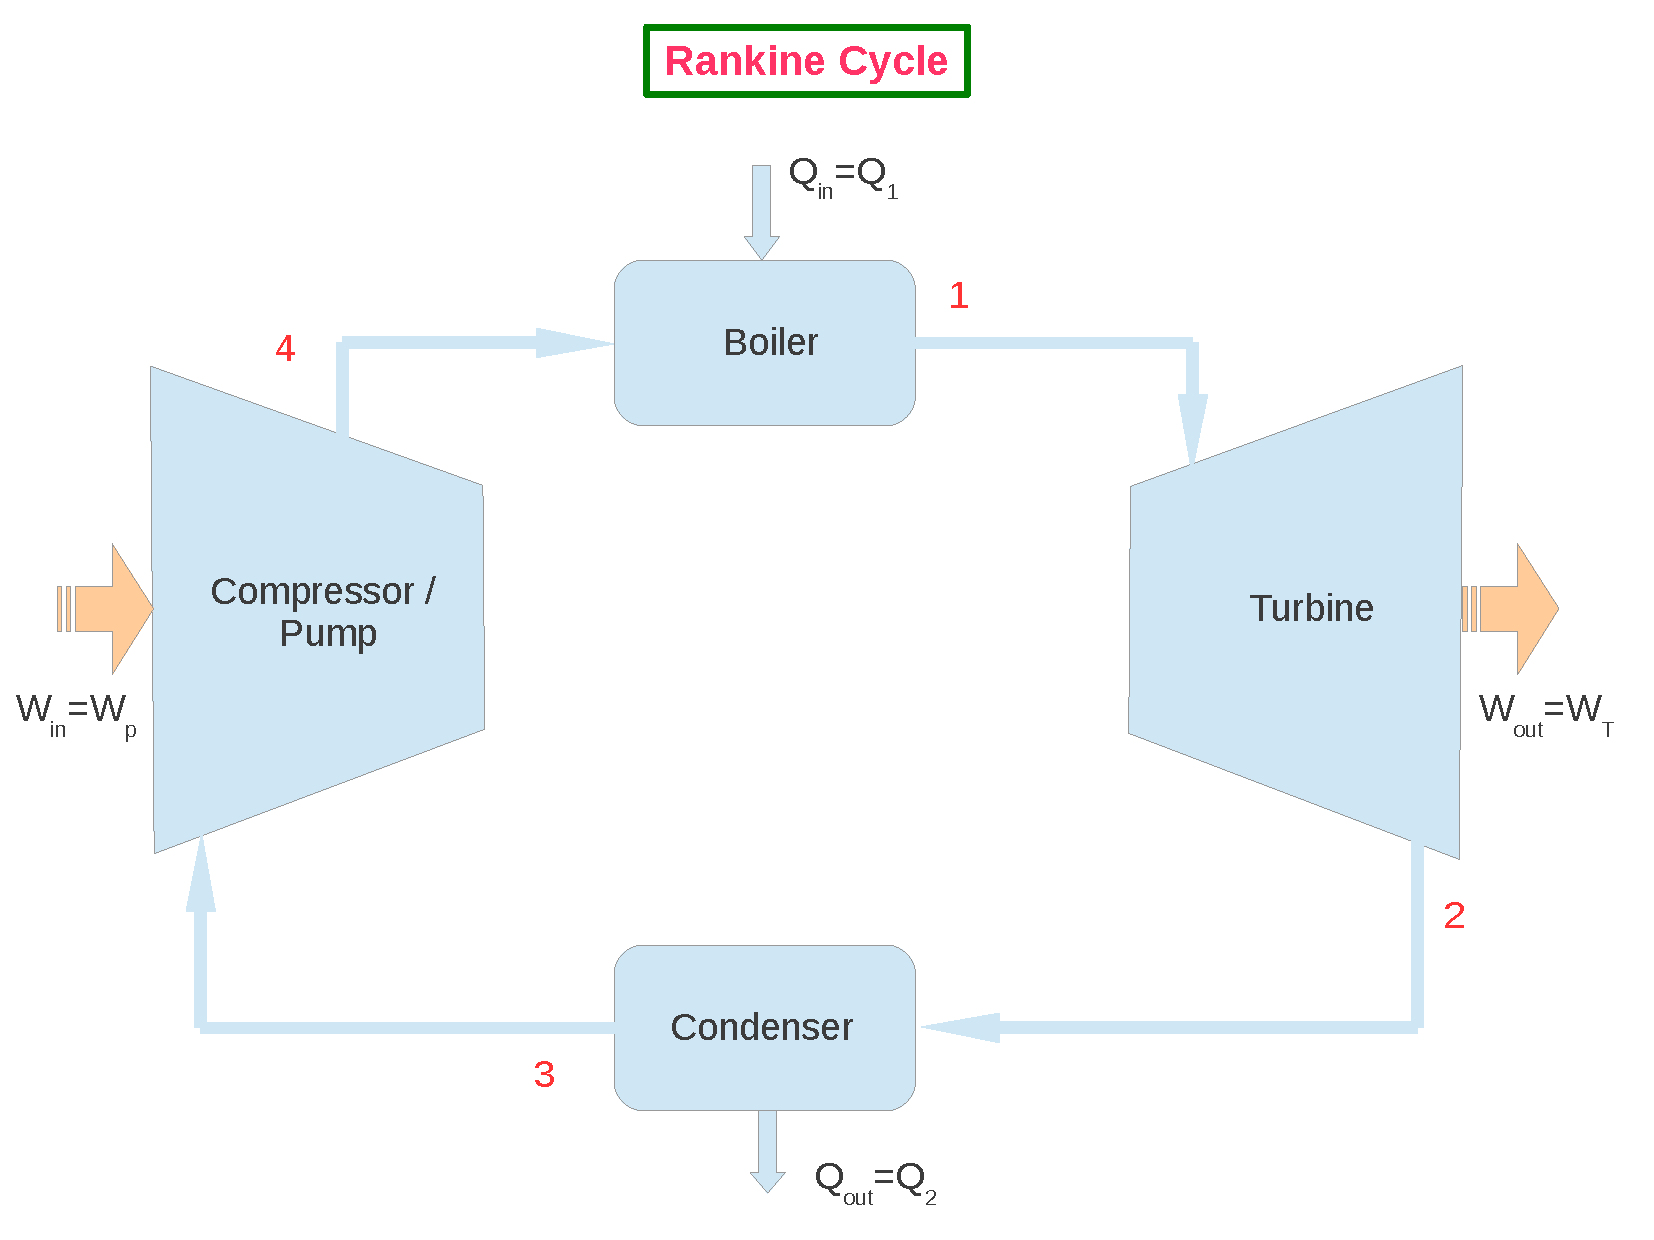
\includegraphics[width=7.5cm,clip]{./Pics/Simple_Rankine_Cycle}
     \end{center}
    \end{figure}  
   \end{column}
   \begin{column}[l]{0.4\linewidth}
    \begin{enumerate}
     \item <1->\textcolor{blue}{Rankine Cycle} is the ideal cycle for vapour power plants.
     \item <2-> The RC does not involve any internal irreversibilities and consists of the following four processes:
    \end{enumerate}
   \end{column}
  \end{columns}
 \normalsize
\end{frame}



%%%
%%% Slide
%%%
\begin{frame}
 \frametitle{Rankine Cycle}
 %\scriptsize
 \begin{columns}
   \begin{column}[c]{0.6\linewidth}
    \begin{figure}%
     \begin{center}
      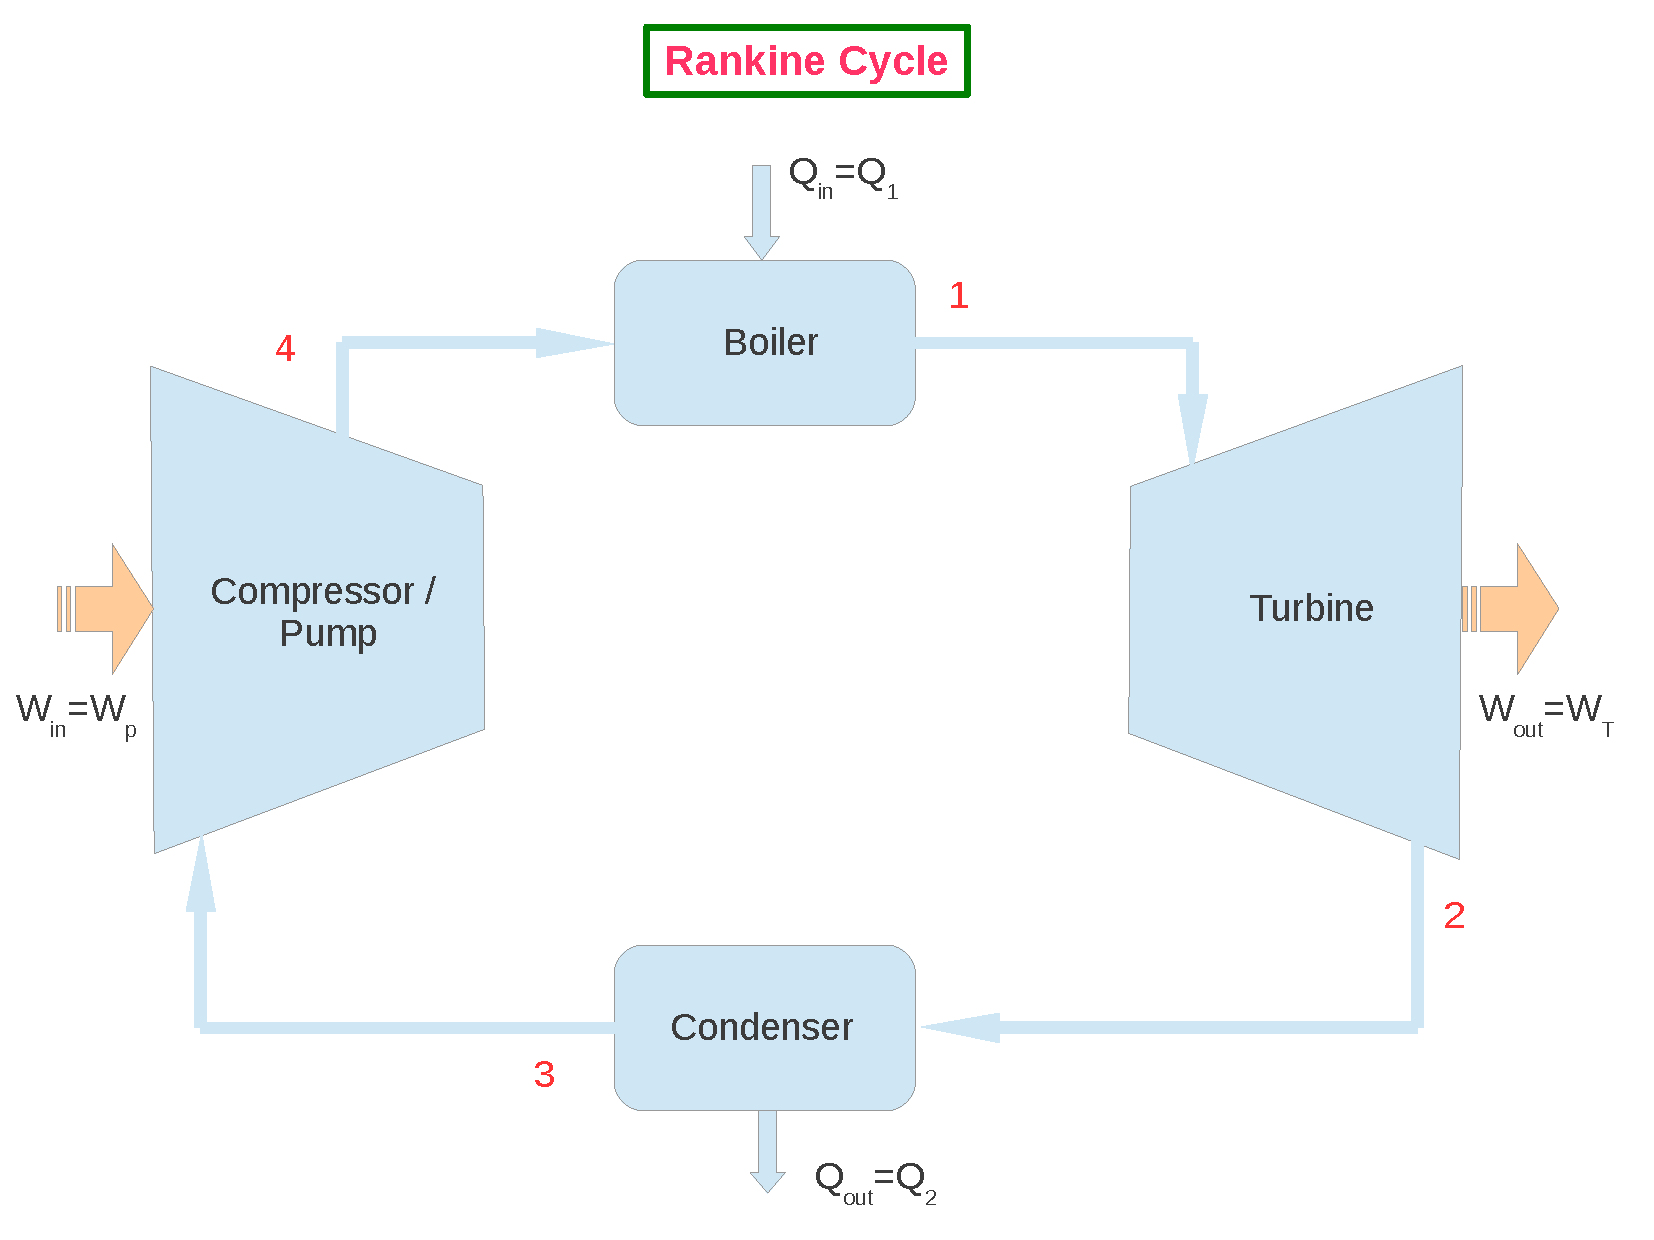
\includegraphics[width=7.5cm,clip]{./Pics/Simple_Rankine_Cycle}
     \end{center}
    \end{figure}  
   \end{column}
   \begin{column}[l]{0.4\linewidth}
     \begin{itemize}%\scriptsize
      \item <3-> \textcolor{red}{Process 1-2}: reversible adiabatic expansion in the turbine (or steam engine);
      \item <4-> \textcolor{red}{Process 2-3}: constant-pressure heat transfer in the condenser;
      \item <5-> \textcolor{red}{Process 3-4}: reversible adiabatic pumping process in the feed pump;
      \item <6-> \textcolor{red}{Process 4-1}: constant-pressure heat transfer in the boiler.  
     \end{itemize}
   \end{column}
  \end{columns}
 \normalsize
\end{frame}




%%%
%%% Slide
%%%
\begin{frame}
 \frametitle{Rankine Cycle: {\it pv}, {\it Ts} and {\it hs} Diagrams}
 %\scriptsize
 \begin{columns}
   \begin{column}[c]{0.55\linewidth}
    \begin{figure}%
     \begin{center}
      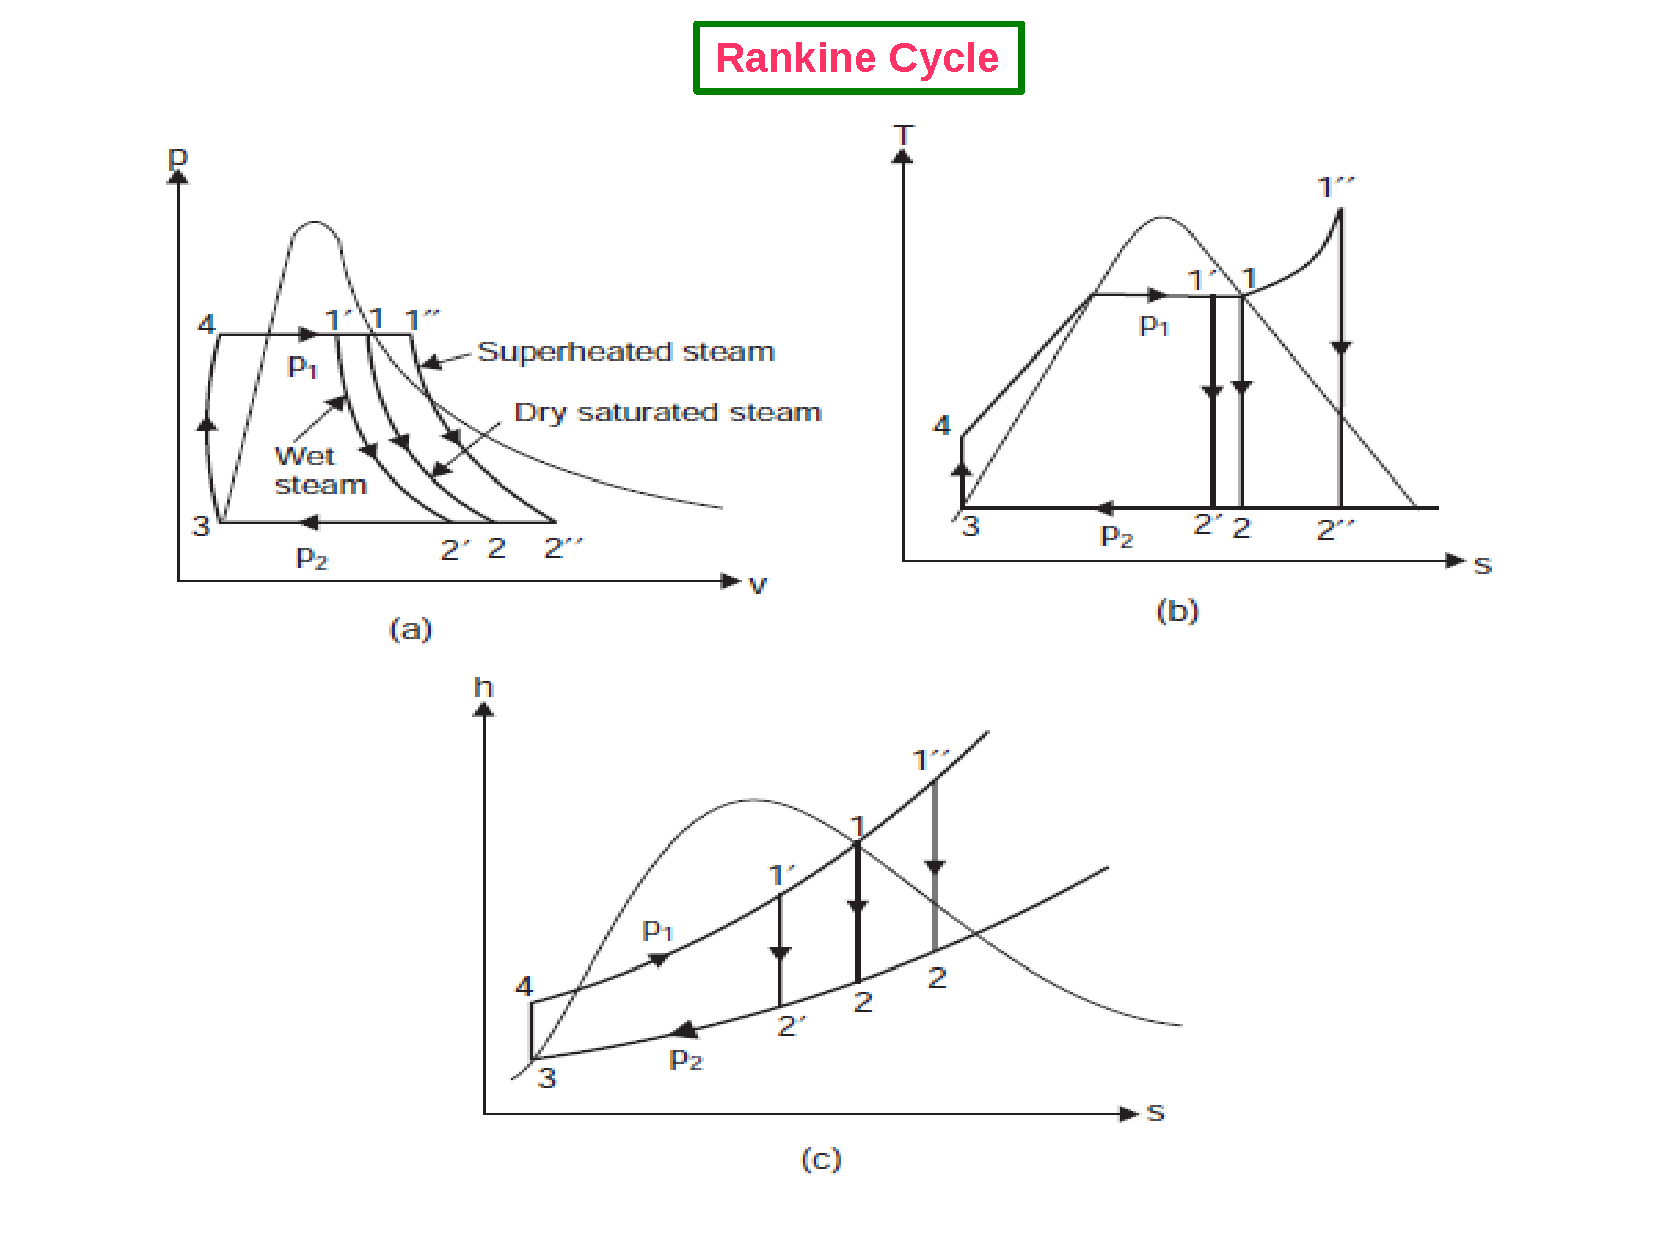
\includegraphics[width=7.5cm,clip]{./Pics/Simple_Rankine_Cycle_Diagrams}
     \end{center}
    \end{figure}  
   \end{column}
   \begin{column}[l]{0.45\linewidth}
    \begin{figure}%
     \begin{center}
      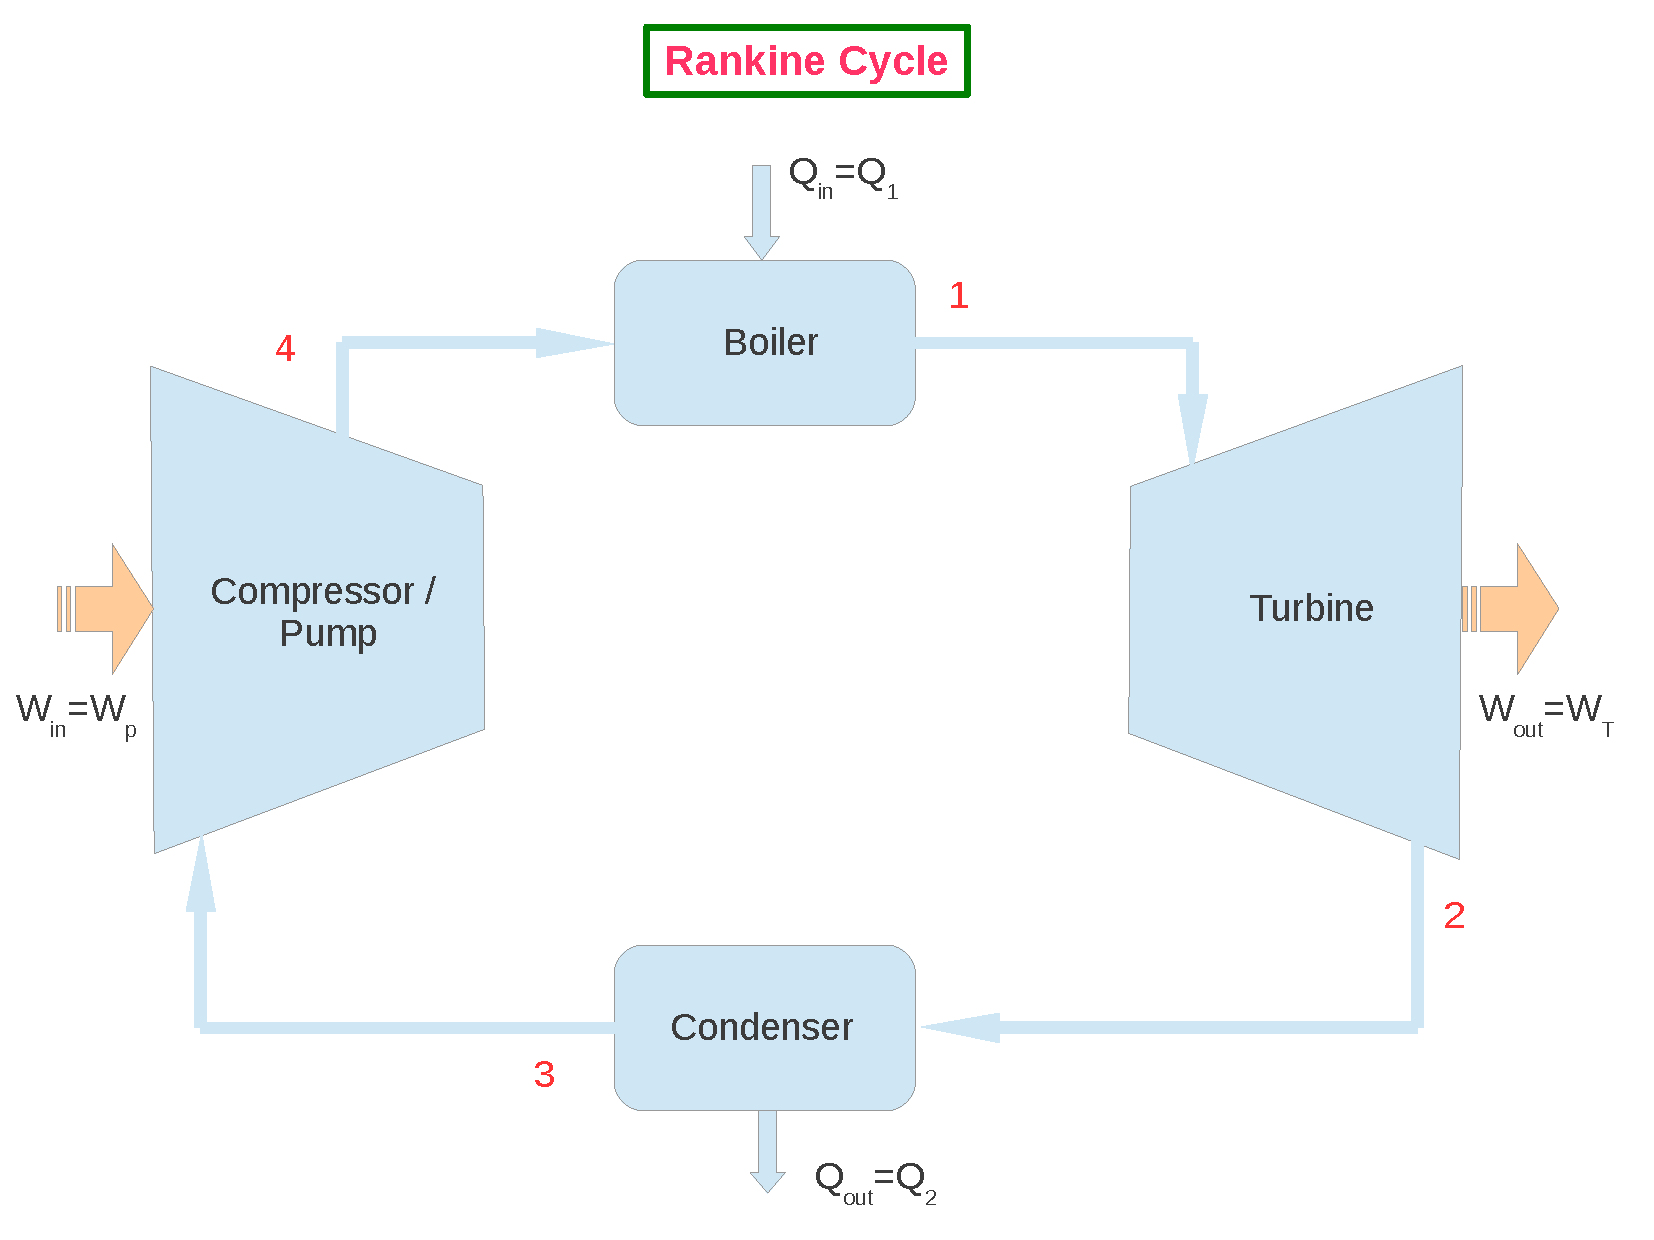
\includegraphics[width=5.5cm,clip]{./Pics/Simple_Rankine_Cycle}
     \end{center}
    \end{figure} 
   \end{column}
  \end{columns}
\end{frame}




%%%
%%% Slide
%%%
\begin{frame}
 \frametitle{Rankine Cycle: Calculating energy conservation}
 %\scriptsize  
  \begin{columns}
   \begin{column}[c]{0.4\linewidth}
    \begin{itemize}
     \item <1-> Calculations within a control volume with 1kg of fluid:
      \begin{enumerate}[(a)] %\scriptsize  
       \item <2->Boiler:\\
        $h_{f_{4}} + Q_{1} = h_{1} \Longrightarrow \textcolor{blue}{Q_{1}=h_{1}-h_{f_{4}}}$
       \item <3->Turbine:\\
        $h_{1} = W_{T} +h_{2} \Longrightarrow \textcolor{blue}{W_{T} =h_{1}-h_{2}}$
       \item <4->Condenser:\\
        $h_{2}=Q_{2}+h_{f_{3}} \Longrightarrow \textcolor{blue}{Q_{2}=h_{2}-h_{f_{3}}}$
       \item <5->Pump:\\
        $h_{f_{3}}+W_{P}=h_{f_{4}} \Longrightarrow \textcolor{blue}{W_{P}=h_{f_{4}}-h_{f_{3}}}$
      \end{enumerate}
     \end{itemize}
    \end{column}
    \begin{column}[c]{0.6\linewidth}
    %\scriptsize  
     \begin{figure}%
      \begin{center}
       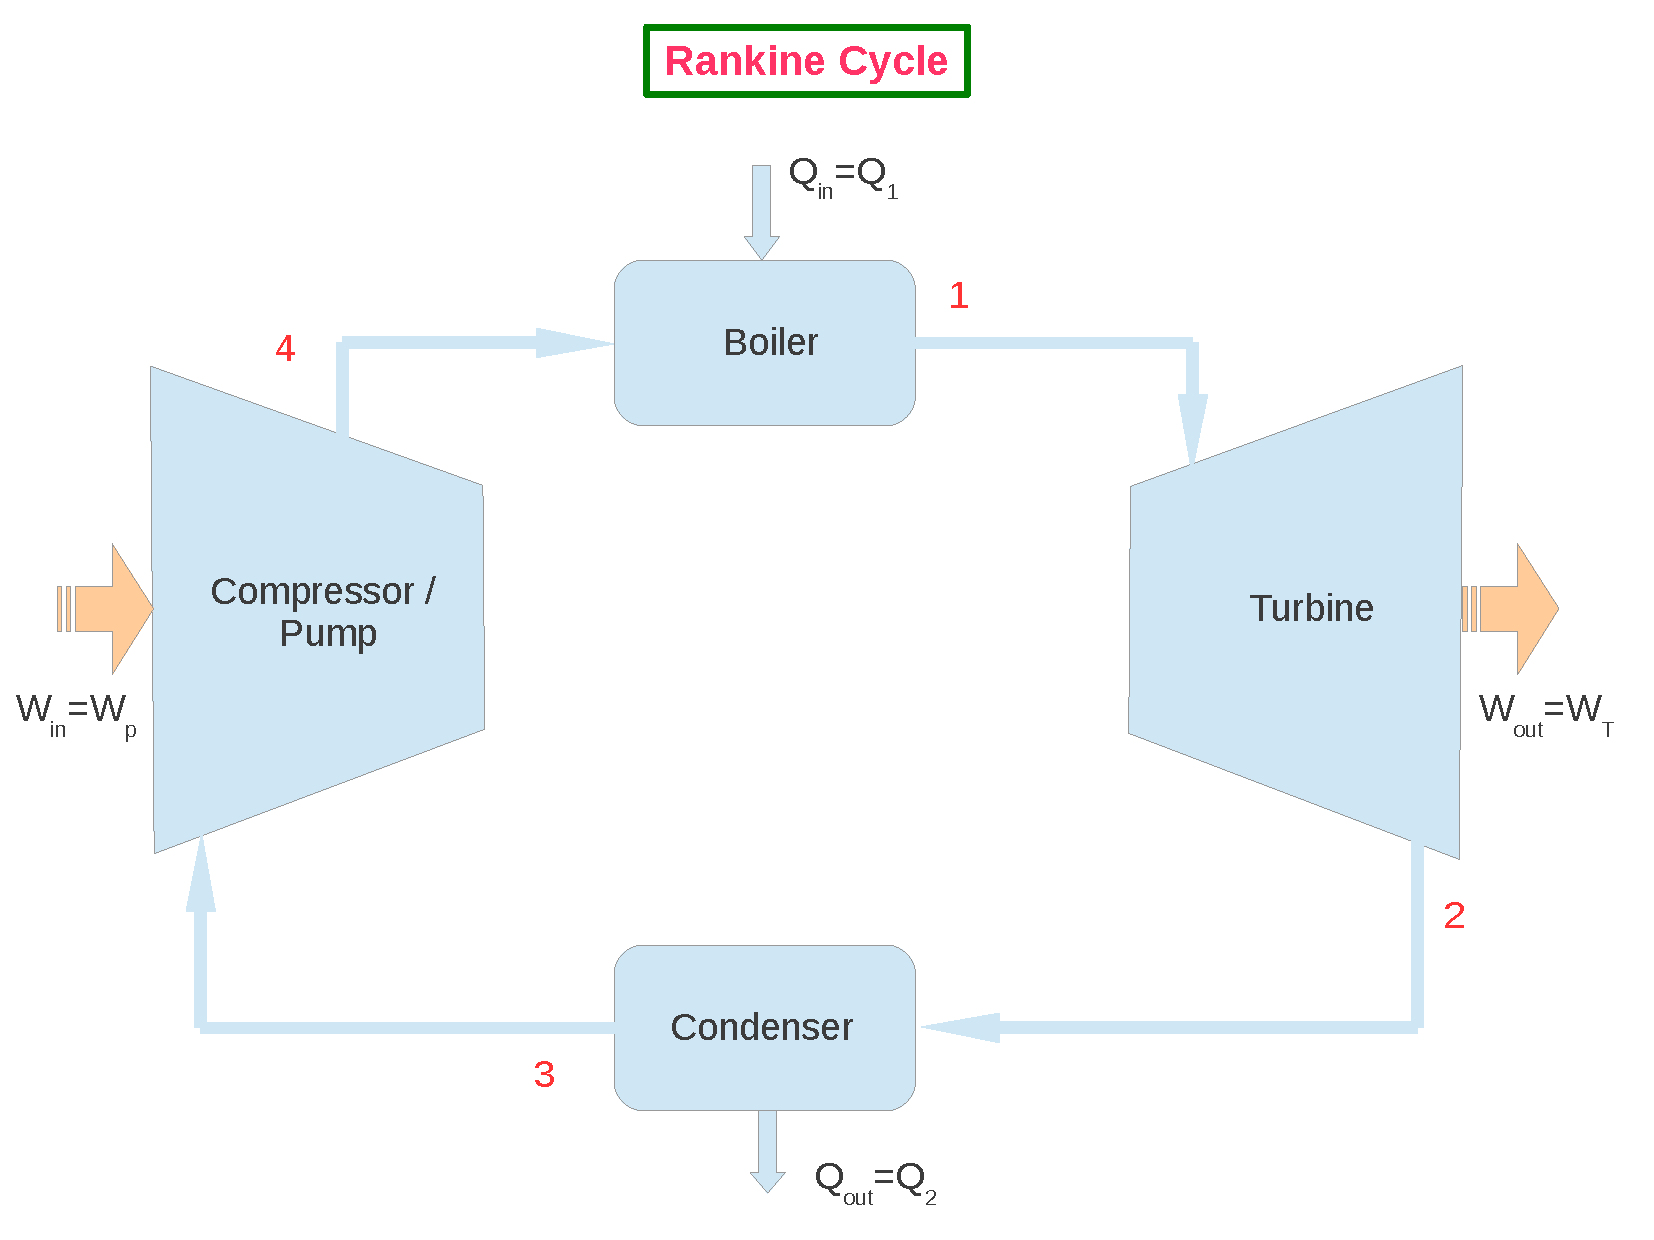
\includegraphics[width=6.5cm,clip]{./Pics/Simple_Rankine_Cycle}
      \end{center}
     \end{figure}
    \end{column}
   \end{columns}
 \normalsize
\end{frame}




%%%
%%% Slide
%%%
\begin{frame}
 \frametitle{Rankine Cycle: Calculating energy conservation}
 %\scriptsize  
  \begin{columns}
   \begin{column}[c]{0.4\linewidth}
    \begin{itemize}
      \item <1-> And the \textcolor{red}{efficiency of Rankine cycle} is,
       $\eta_{\text{Rankine}}=\displaystyle\frac{W_{net}}{Q_{1}}=\displaystyle\frac{W_{T}-W_{P}}{Q_{1}}$ \\
       $\textcolor{blue}{\eta_{\text{Rankine}}=\displaystyle\frac{\left(h_{1}-h_{2}\right)-\left(h_{f_{4}}-h_{f_{3}}\right)}{h_{1}-h_{f_{4}}}}$
      \item <2-> The pump deals with incompressible liquid water $\Rightarrow$ an increase in pressure leads to small change in density (or specific volume). 
      \item <3-> Thus for reversible adiabatic compression, $Tds=dh-vdp$ with $ds=0$ therefore,
      % $dh = vdp \Longrightarrow \Delta h = v\Delta p \Longrightarrow h_{f_{4}}-h_{f_{3}}=v_{3}\left(p_{1}-p_{2}\right)$ 
     \end{itemize}
    \end{column}
    \begin{column}[c]{0.6\linewidth}
    %\scriptsize  
     %\begin{itemize}
      %\item <8-> Thus for reversible adiabatic compression, $Tds=dh-vdp$ with $ds=0$ therefore,
      %\item<8-> $dh = vdp \Longrightarrow \Delta h = v\Delta p \Longrightarrow h_{f_{4}}-h_{f_{3}}=v_{3}\left(p_{1}-p_{2}\right)$ 
      %\item <9-> The pump term, $\left(h_{f_{4}}-h_{f_{3}}\right)$, is very small (if compared to the work produced by the turbine -- $W_{T}$) and therefore it is usually neglected. In particular when the {\it boiler pressure is low}.
      %\item <10-> The {\it efficiency of the Rankine cycle} is \\
      %   $ \textcolor{red}{\eta_{\text{Rankine}}=\displaystyle\frac{h_{1}-h_{2}}{h_{1}-h_{f_{4}}}}$ 
     %\end{itemize}
     \begin{figure}%
      \begin{center}
       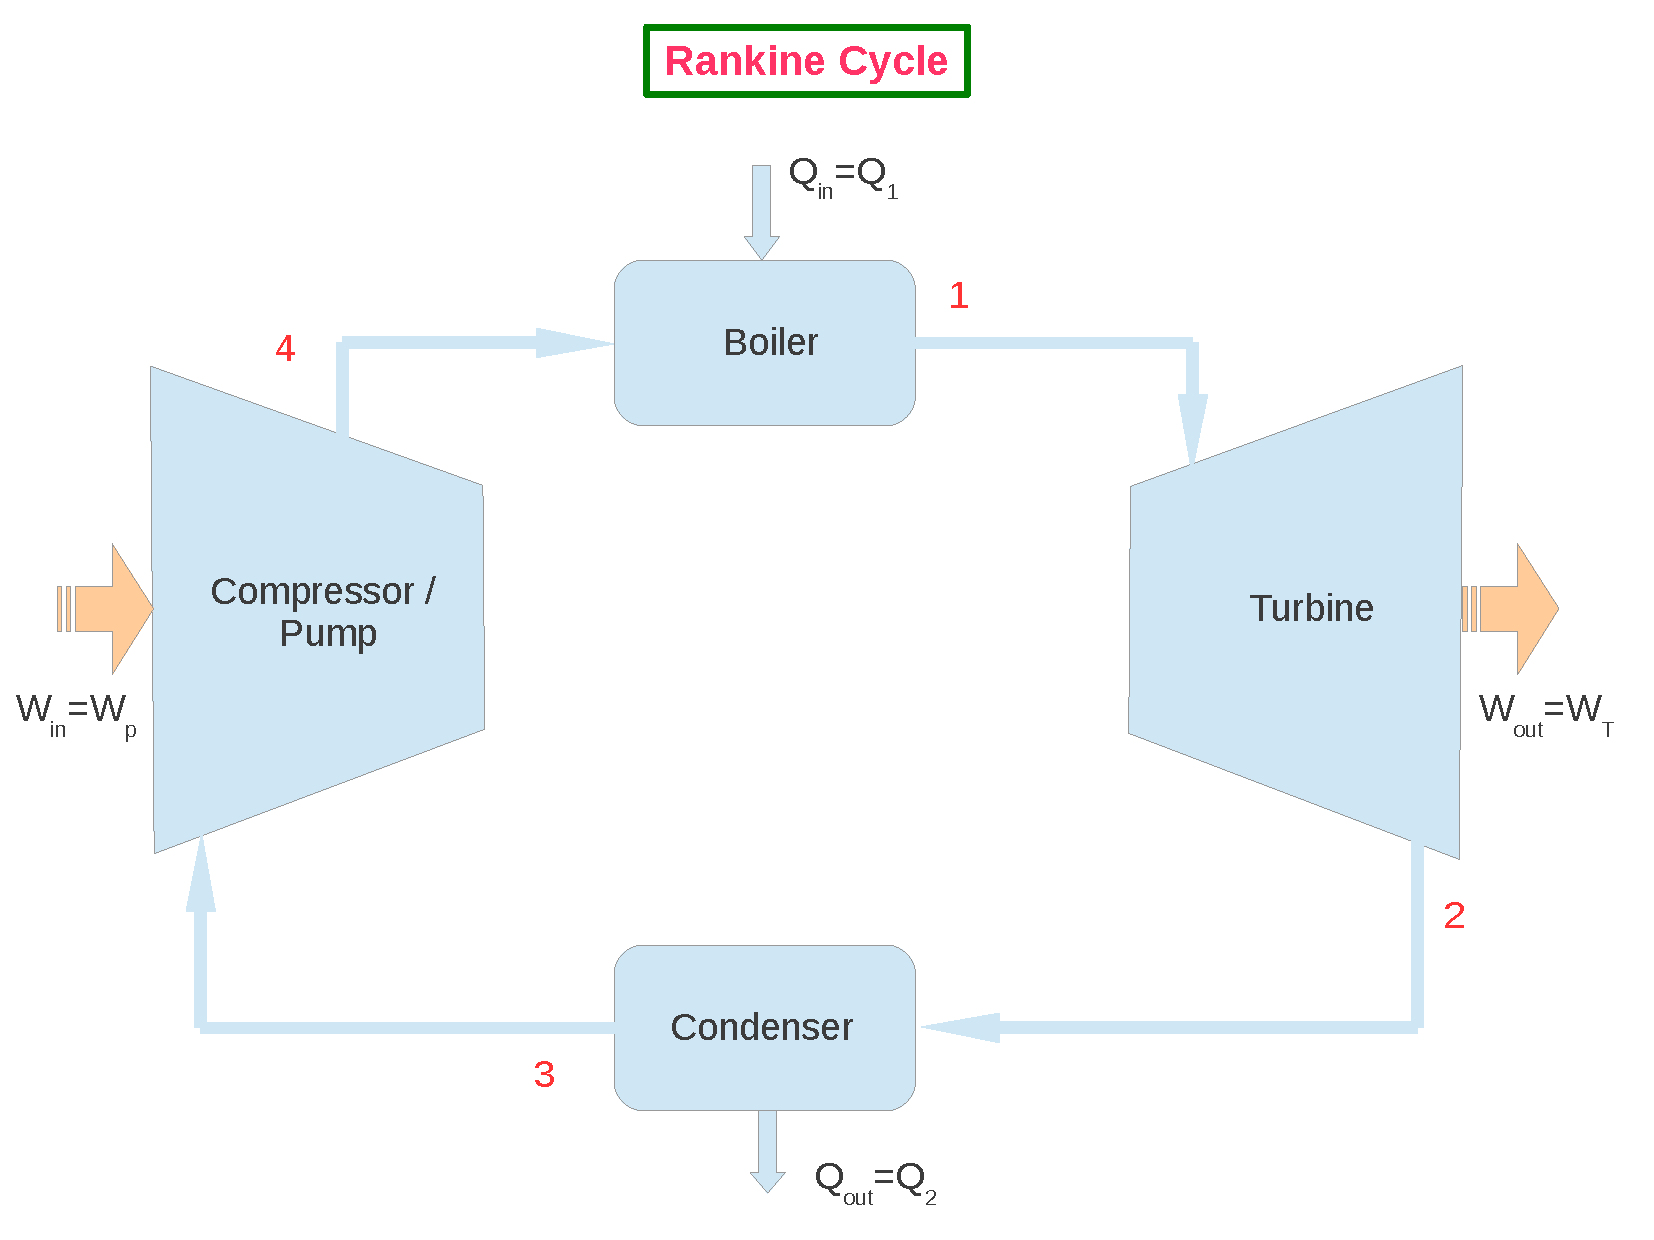
\includegraphics[width=6.5cm,clip]{./Pics/Simple_Rankine_Cycle}
      \end{center}
     \end{figure}
    \end{column}
   \end{columns}
\begin{center}
     %  $dh = vdp \;\; \textcolor{red}{\Longrightarrow}\;\; \Delta h = v\Delta p \;\;\textcolor{red}{\Longrightarrow}\;\; h_{f_{4}}-h_{f_{3}}=v_{3}\left(p_{1}-p_{2}\right)$ 
       $dh = vdp \;\; \textcolor{red}{\Longrightarrow}\;\; \Delta h = v\Delta p \;\;\textcolor{red}{\Longrightarrow}\;\; h_{f_{4}}-h_{f_{3}}=v_{3}\left(p_{4}-p_{3}\right)$ 
\end{center}
 \normalsize
\end{frame}


%%%
%%% Slide
%%%
\begin{frame}
 \frametitle{Rankine Cycle: Calculating energy conservation}
 %\scriptsize  
  \begin{columns}
   \begin{column}[c]{0.4\linewidth}
    \begin{itemize}
      %\item <8-> Thus for reversible adiabatic compression, $Tds=dh-vdp$ with $ds=0$ therefore,
      %\item<8-> $dh = vdp \Longrightarrow \Delta h = v\Delta p \Longrightarrow h_{f_{4}}-h_{f_{3}}=v_{3}\left(p_{1}-p_{2}\right)$ 
      \item <1-> The pump term, $\left(h_{f_{4}}-h_{f_{3}}\right)$, is very small (if compared to the work produced by the turbine -- $W_{T}$) and therefore it is usually neglected. In particular when the {\it boiler pressure is low}.
      \item <2-> The {\it efficiency of the Rankine cycle} is
\begin{center}
         %$ \textcolor{red}{\eta_{\text{Rankine}}=\displaystyle\frac{h_{1}-h_{2}}{h_{1}-h_{f_{4}}}}$ 
         $ \textcolor{red}{\eta_{\text{Rankine}}=\displaystyle\frac{h_{1}-h_{2}}{h_{1}-h_{f_{4}}}}$ 
\end{center}
     \end{itemize}
    \end{column}
    \begin{column}[c]{0.6\linewidth}
     \begin{figure}%
      \begin{center}
       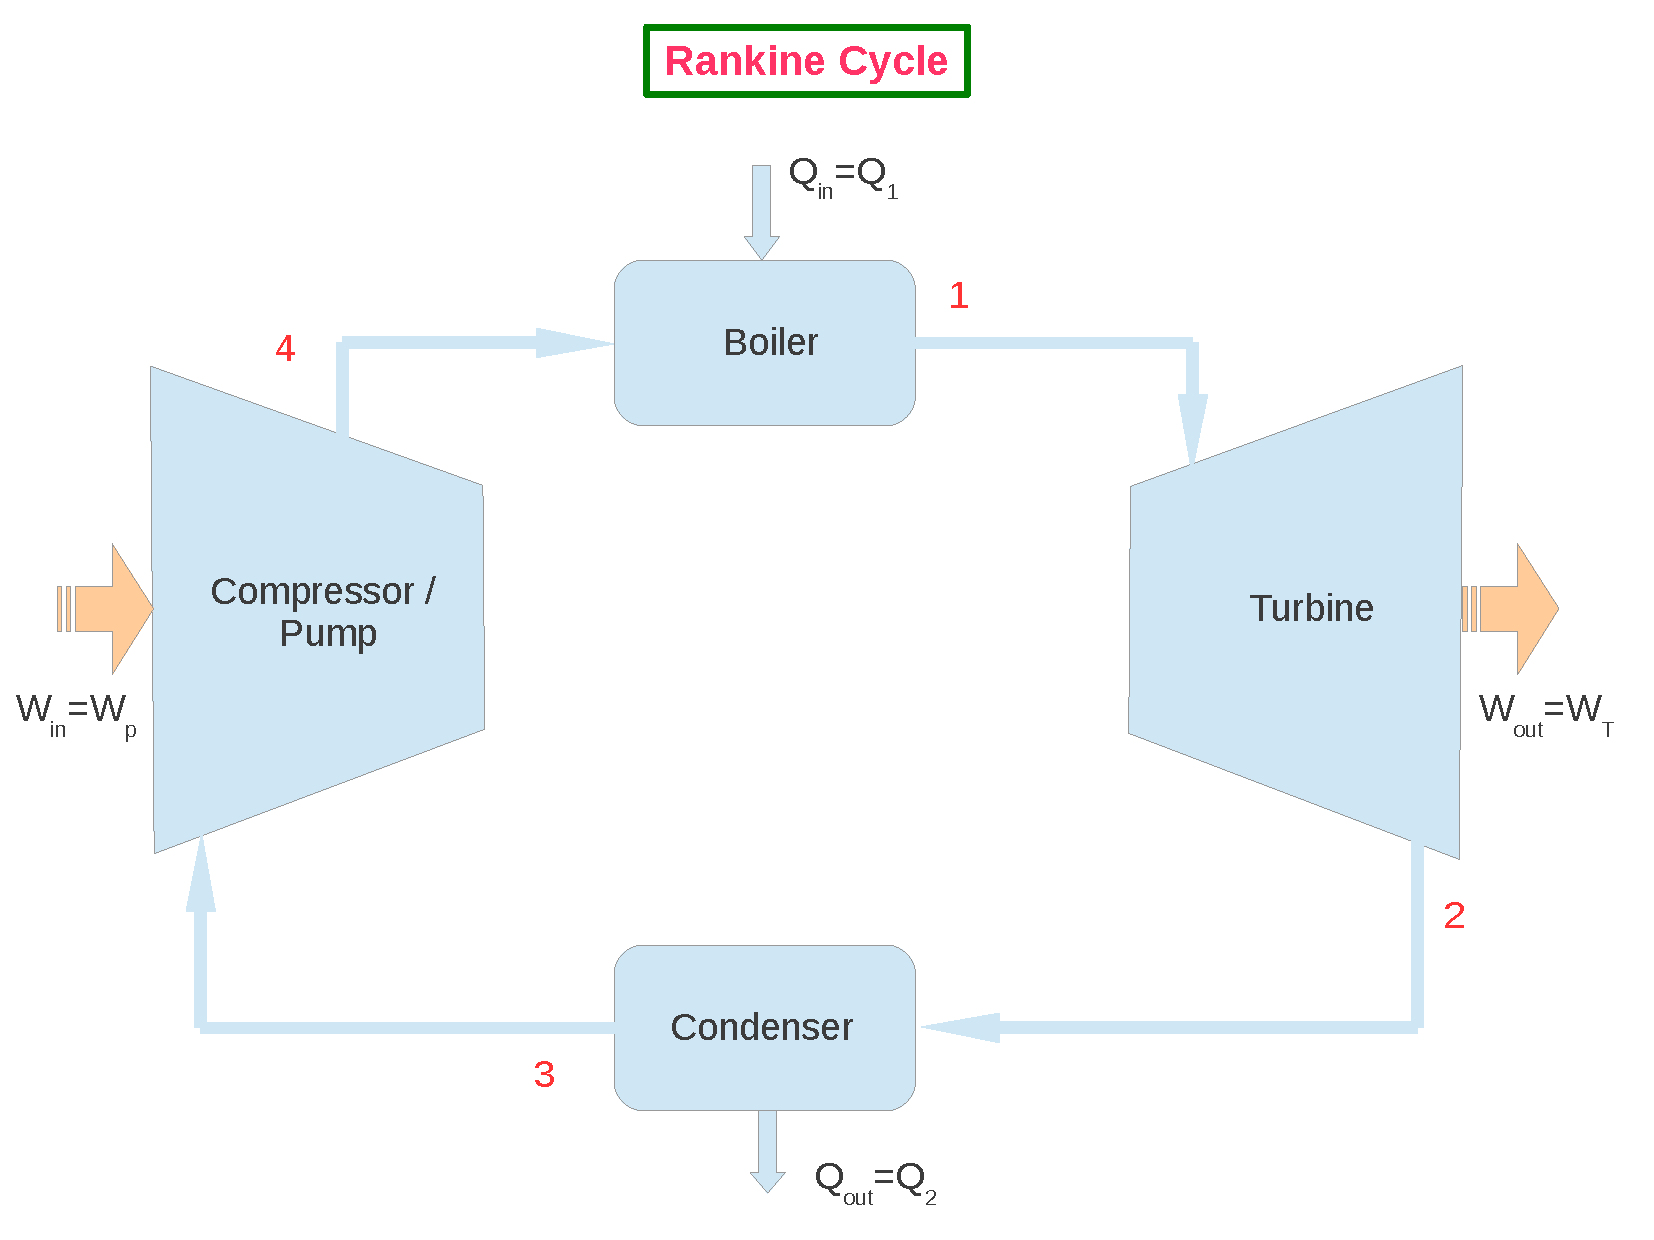
\includegraphics[width=6.5cm,clip]{./Pics/Simple_Rankine_Cycle}
      \end{center}
     \end{figure}
    \end{column}
   \end{columns}
 \normalsize
\end{frame}



%%%
%%% Slide
%%%
\begin{frame}
 \frametitle{Comparison between Rankine and Carnot Cycles}
 %\scriptsize
  \begin{columns}
   \begin{column}[c]{0.4\linewidth}
    \begin{itemize}
     \item <1-> Between the same temperature range $\left(T_{1}\text{ and }T_{2}\right)$ Rankine cycle provides a higher specific work output than a Carnot cycle $\Longrightarrow$ Rankine cycle requires a smaller steam flow rate. 
     \item <2-> However, Rankine cycle requires larger heat transfer rates between the boiler and the condenser.
    \end{itemize}
   \end{column}
   \begin{column}[c]{0.6\linewidth}
    \begin{figure}%
     \begin{center}
      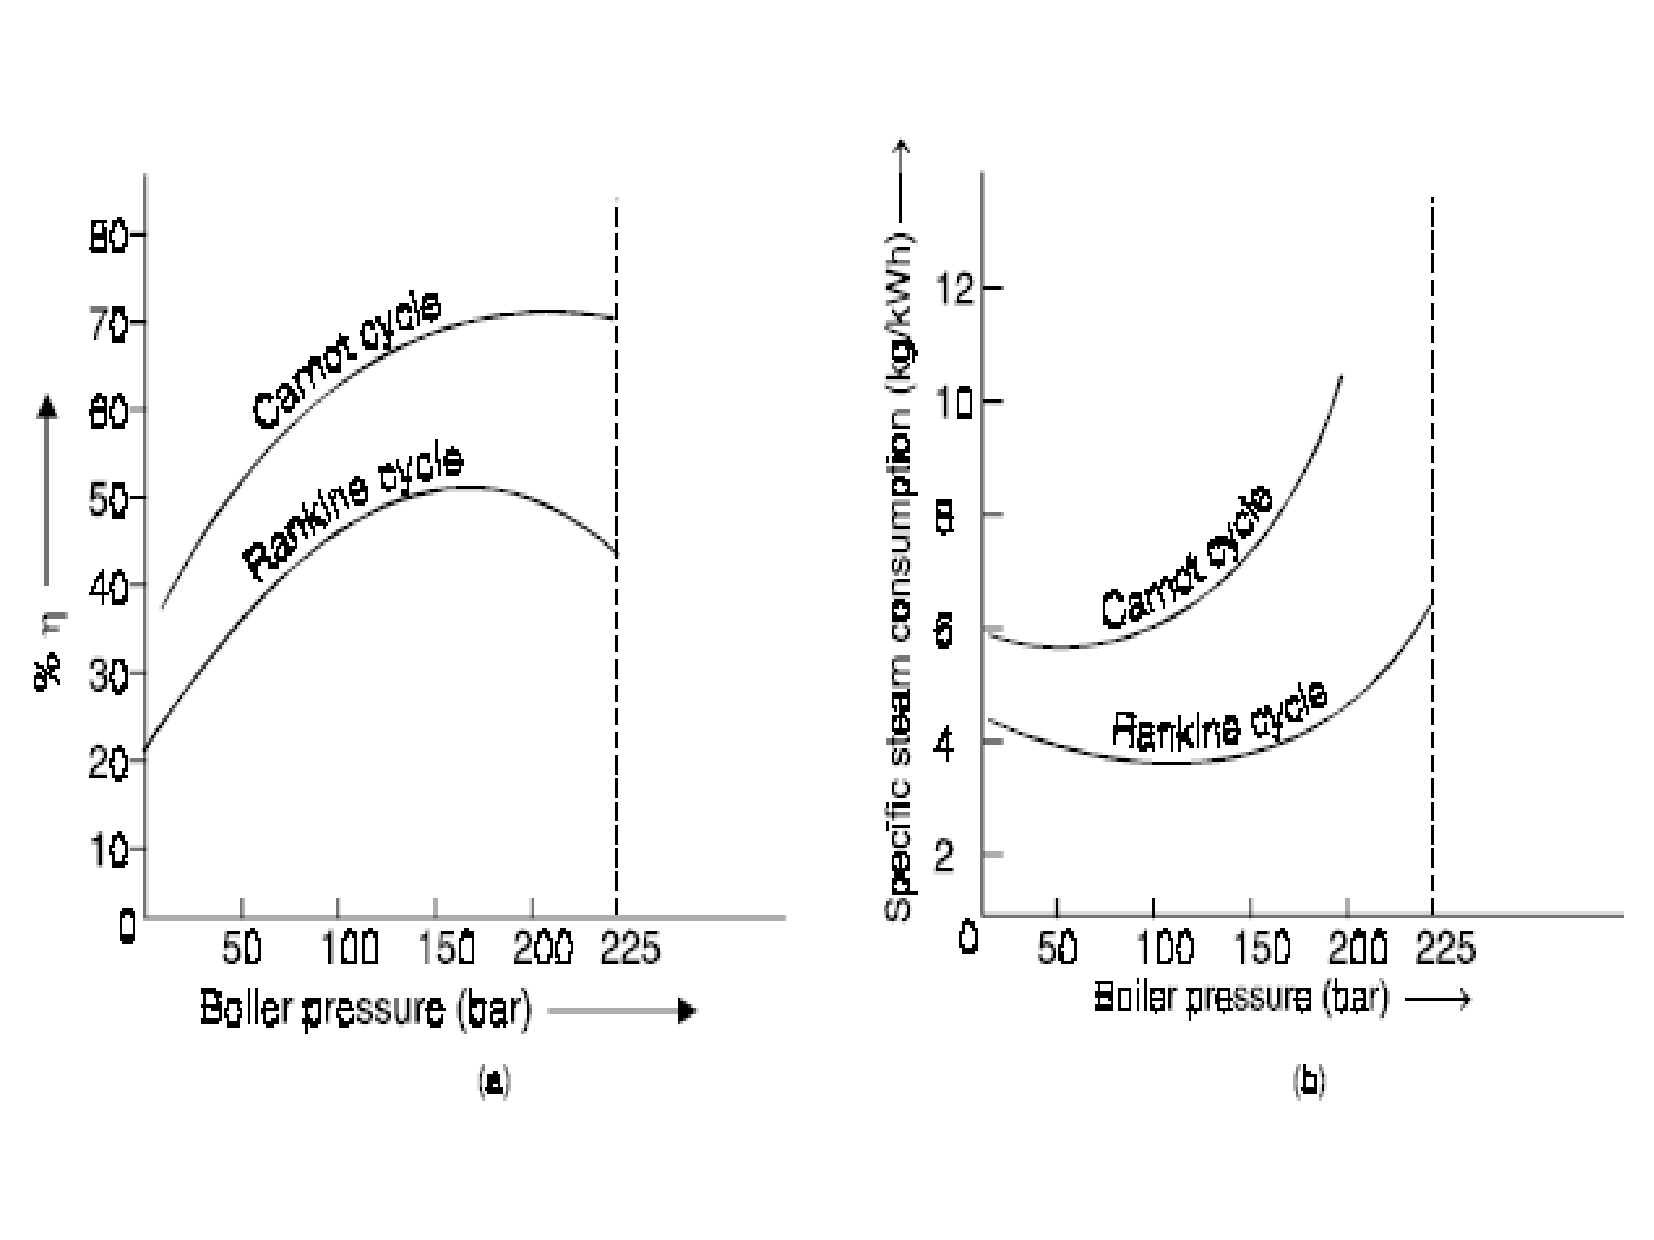
\includegraphics[width=7.5cm,clip]{./Pics/Comparison_Rankine_Carnot}
     \end{center}
    \end{figure}  
   \end{column}
  \end{columns}
 \normalsize
\end{frame}





%%%
%%% Slide
%%%
\begin{frame}
 \frametitle{Comparison between Rankine and Carnot Cycles}
 %\scriptsize
  \begin{columns}
   \begin{column}[c]{0.4\linewidth}
    \begin{itemize}%\scriptsize
     \item <1-> In Rankine cycles, only part of the heat is supplied isothermally at constant high temperature $T_{1}$, therefore \textcolor{blue}{the efficiency is lower than that of Carnot cycle}. The efficiency of the Rankine cycle will approach that of the Carnot cycle more nearly if the superheat temperature rise is reduced.
     \item <2-> The advantage of using pump to feed liquid to the boiler instead to compressing a wet vapour is because the work for steam compression is larger than pumping liquid.
    \end{itemize}
   \end{column}
   \begin{column}[c]{0.6\linewidth}
    \begin{figure}%
     \begin{center}
      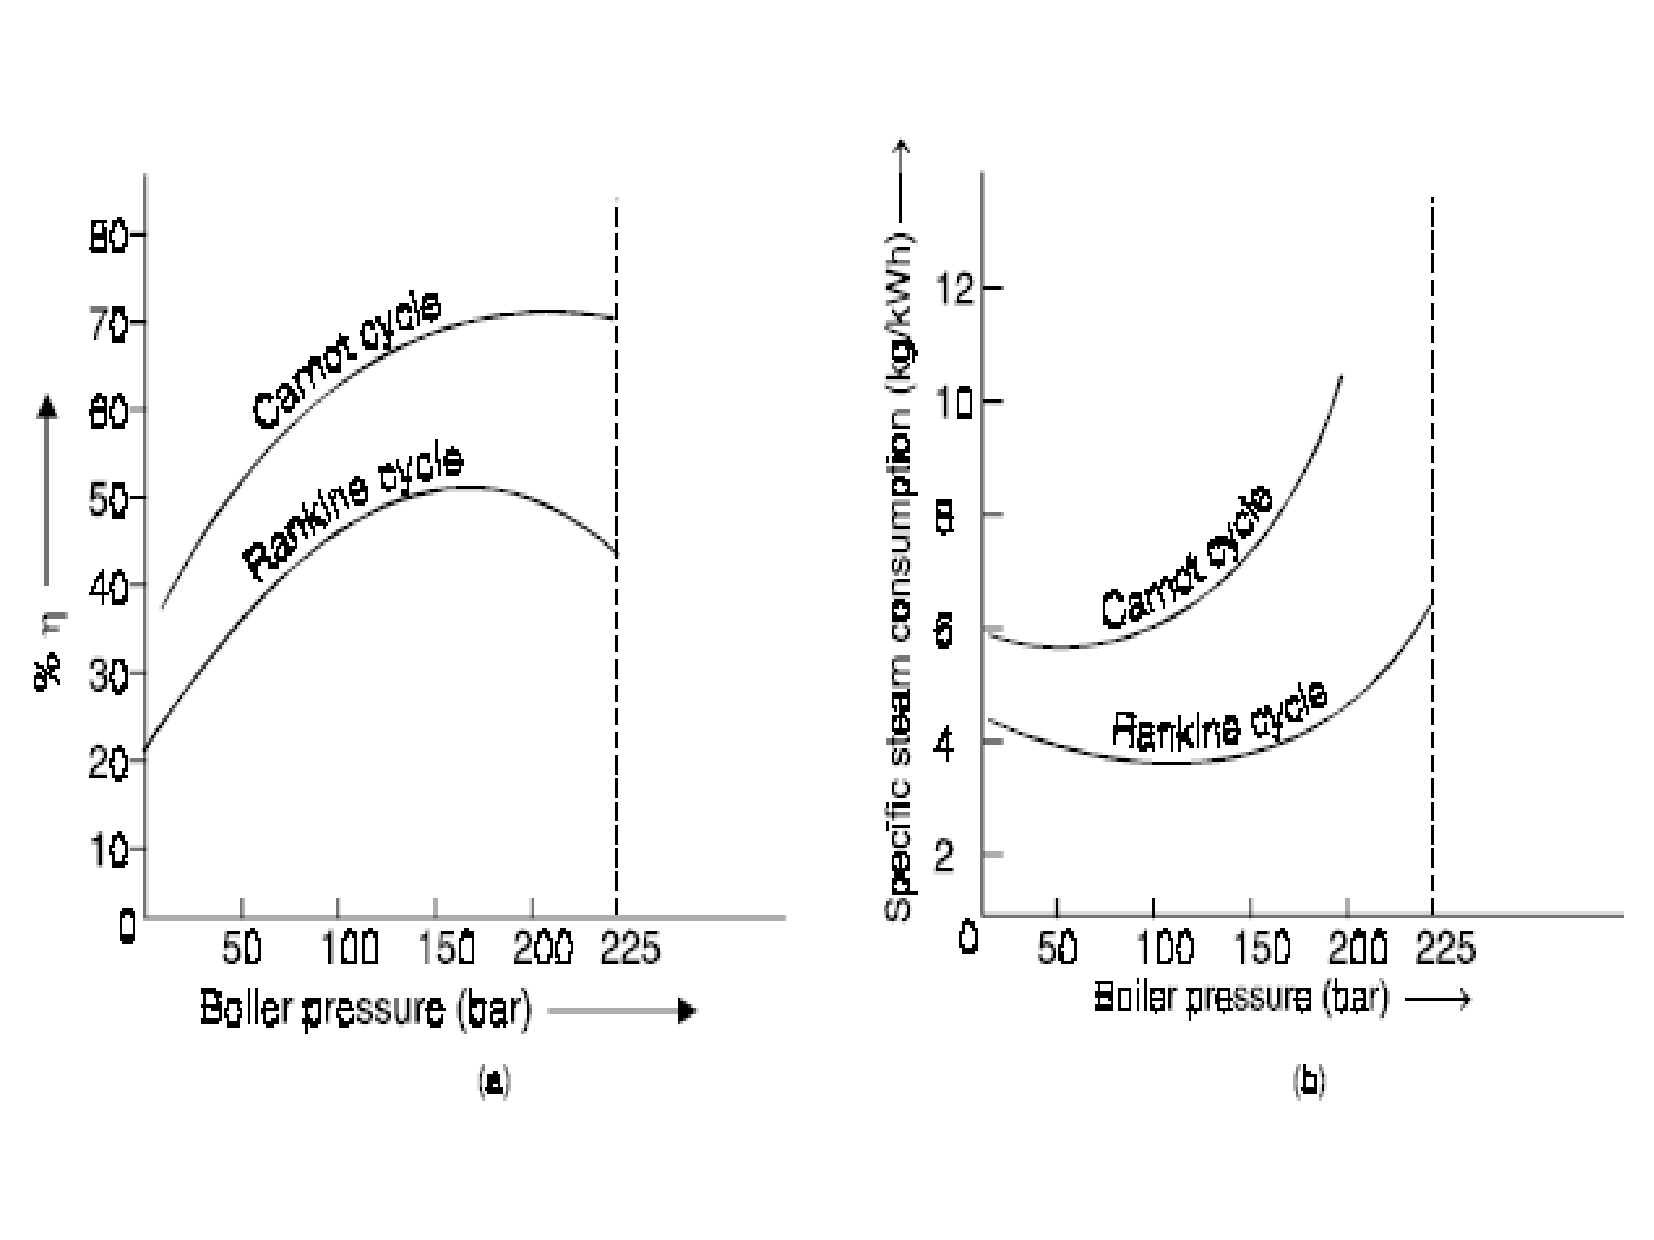
\includegraphics[width=7.5cm,clip]{./Pics/Comparison_Rankine_Carnot}
     \end{center}
    \end{figure}  
   \end{column}
  \end{columns}
 \normalsize
\end{frame}


%%%
%%% Slide
%%%
\begin{frame}
 \frametitle{Ideal {\it versus} Real Cycles}
 %\scriptsize
      Differences between real vapour cycles and the ideal Rankine cycle are mainly due to the following irreversibilities: 
  \begin{columns}

   \begin{column}[c]{0.4\linewidth}
      \begin{itemize}%\scriptsize
      \item <1-> \textcolor{blue}{Fluid friction} results in pressure drop in the boiler, condenser and pipes. Steam leaves the boiler at a pressure lower than expected. 
      \item <2-> Fluid pressure at the turbine inlet is also lower than that at the boiler exit due to pressure drop between pipes. 
    \end{itemize}
   \end{column}
   \begin{column}[c]{0.6\linewidth}
    \begin{figure}%
     \begin{center}
      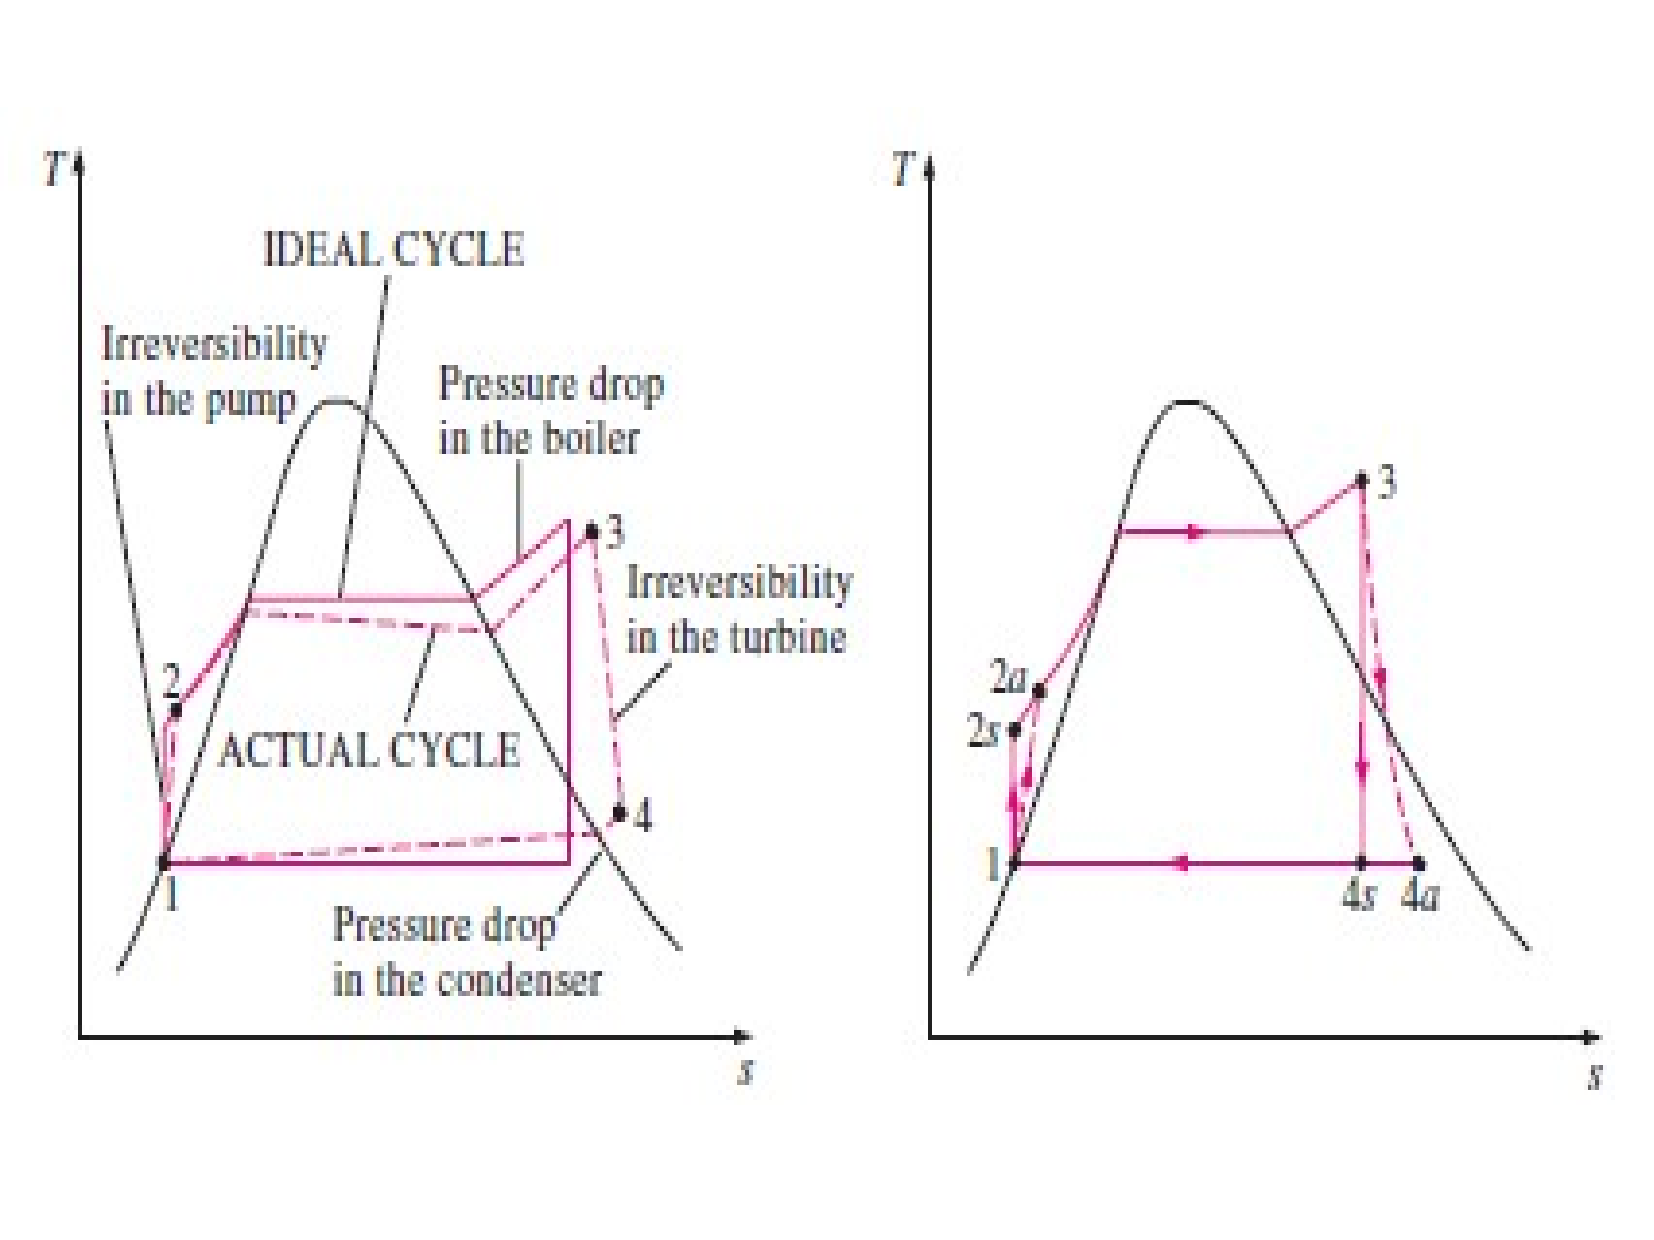
\includegraphics[width=7.5cm,clip]{./Pics/Rankine_vs_Real}
     \end{center}
    \end{figure}  
   \end{column}

  \end{columns}
 \normalsize
\end{frame}




%%%
%%% Slide
%%%
\begin{frame}
 \frametitle{Ideal {\it versus} Real Cycles}
 %\scriptsize
      %Differences between real vapour cycles and the ideal Rankine cycle are mainly due to the following irreversibilities: 
  \begin{columns}

   \begin{column}[c]{0.4\linewidth}
      \begin{itemize}%\scriptsize
      \item <1-> Pressure drop in the condenser is usually negligible. In order to mitigate these pressure drops throughout power cycles, water must be pumped to a pressure higher than the required in the ideal cycle. 
      \item <2-> To this end, a more powerful pump (and therefore larger worker input to the pump) is needed, increasing the energy cost.  
    \end{itemize}
   \end{column}
   \begin{column}[c]{0.6\linewidth}
    \begin{figure}%
     \begin{center}
      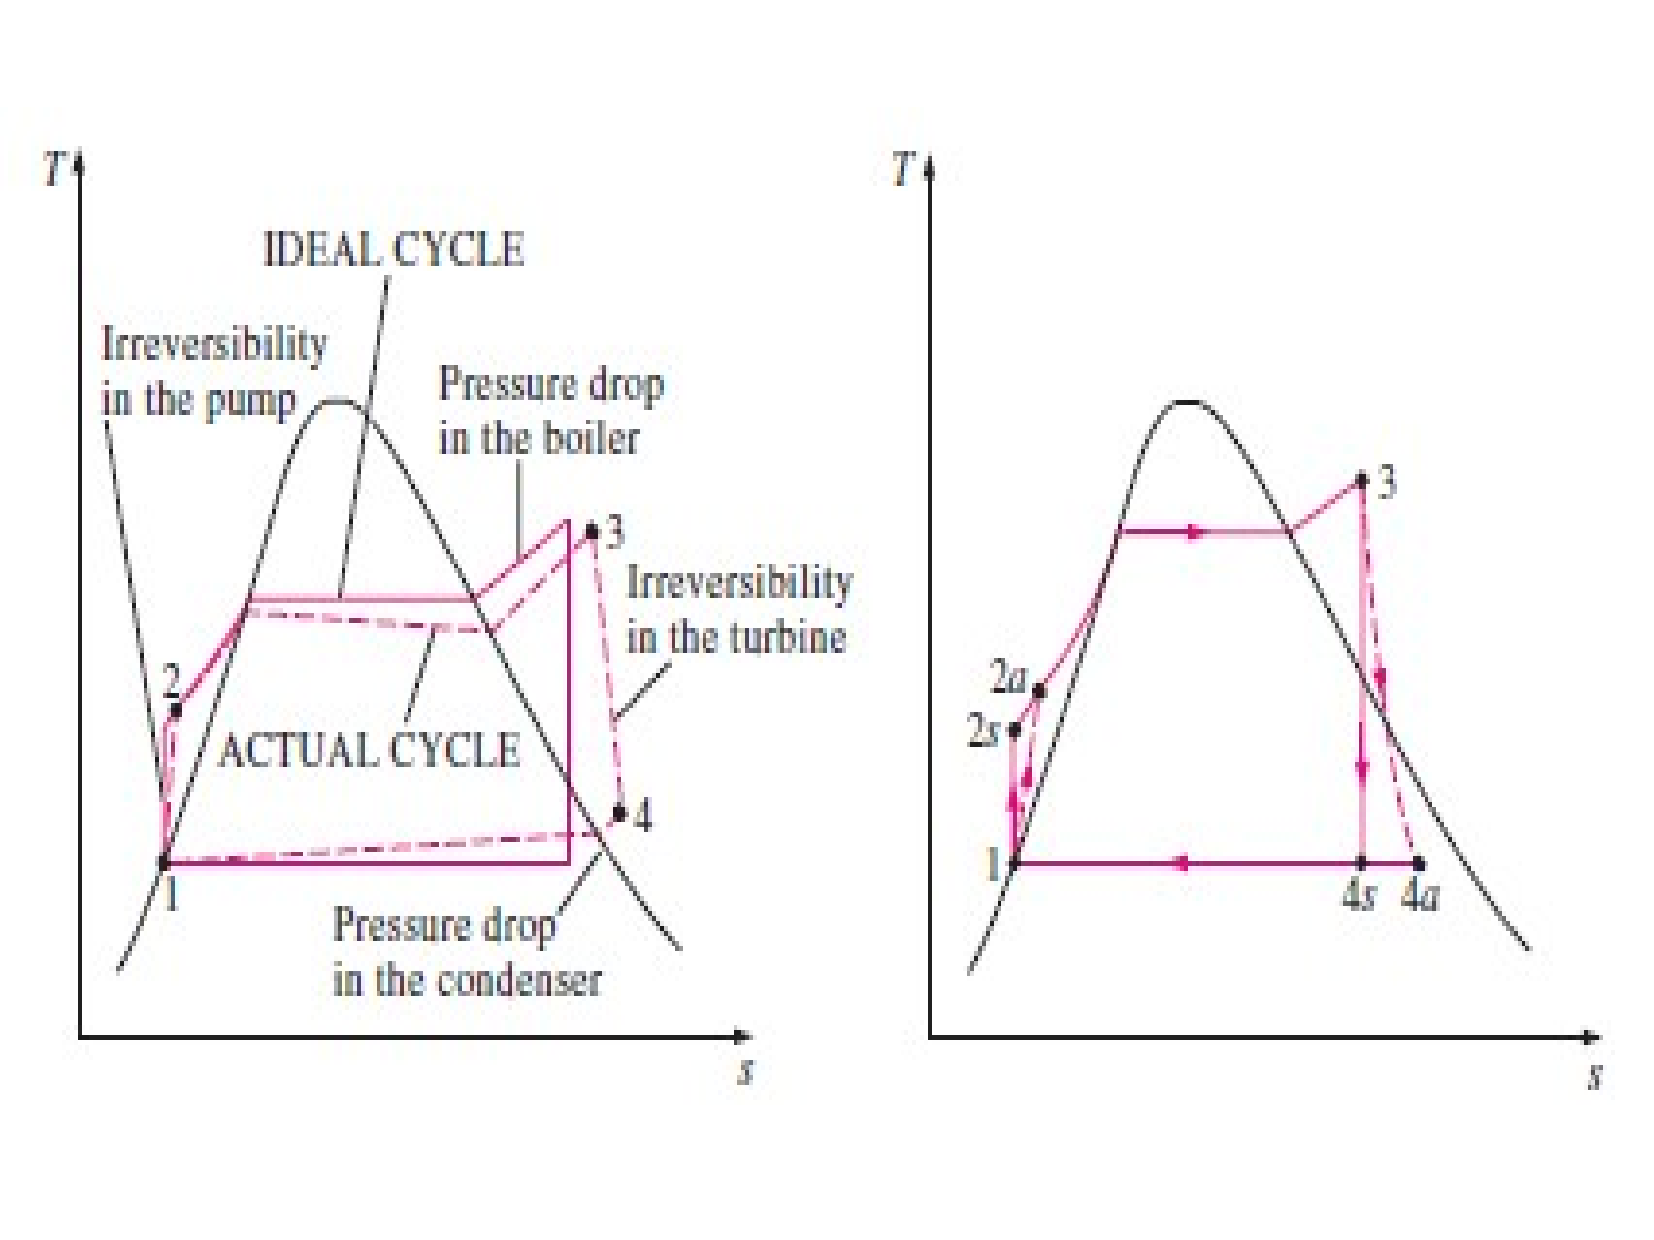
\includegraphics[width=7.5cm,clip]{./Pics/Rankine_vs_Real}
     \end{center}
    \end{figure}  
   \end{column}

  \end{columns}
 \normalsize
\end{frame}



%%%
%%% Slide
%%%
\begin{frame}
 \frametitle{Ideal {\it versus} Real Cycles}
 %\scriptsize
      \begin{itemize}%\scriptsize
      \item <2-> \textcolor{blue}{Heat loss} from the steam to the surroundings is also a major factor. In order to keep the same level of net work output, an extra amount of heat needs to be transferred into the steam in the boiler to compensate for heat losses -- this leads to a decrease in the cycle efficiency.
       \item <3-> \textcolor{blue}{Turbine-Pump flow linkage:} the pump requires a larger work input and the turbine produces a smaller work output as a result of irreversibilities. In ideal cycles, the flow through these devices is assumed isentropic. Deviation from isentropic conditions can be obtained from isentropic efficiencies:\\
     \medskip
     \textcolor{red}{$\eta_{P}=\displaystyle\frac{W_{s}}{W_{a}}=\displaystyle\frac{h_{2s}-h_{1}}{h_{2a}-h_{1}}$}\\
     \medskip
     \textcolor{red}{$\eta_{T}=\displaystyle\frac{W_{a}}{W_{s}}=\displaystyle\frac{h_{3}-h_{4a}}{h_{3}-h_{4s}}$}\\
     \medskip
     $2a$ and $4a$ are the actual exit states of the pump and turbine, whereas $2s$ and $4s$ are the corresponding isentropic ideal case.
    \end{itemize}
 \normalsize
\end{frame}




%%%
%%% Slide
%%%
\begin{frame}
 \frametitle{Improving the Efficiency of the Rankine Cycles}
    \begin{enumerate}%\scriptsize
     \item <1-> The efficiency of the Rankine cycle may be improved by:
     \begin{enumerate}[(i)]%\scriptsize
      \item <2-> Increasing the average temperature at which heat is transferred to the working fluid in the boiler or;
      \item <3-> Reducing the temperature at which the heat is transferred from the working fluid in the condenser;
     \end{enumerate} 
     \item <4-> This can be achieved with:
      \begin{enumerate}[(a)]%\scriptsize
       \item <5-> Increasing boiler pressure;
       \item <6-> Use of superheated steam;
       \item <7-> Reducing condenser pressure.
      \end{enumerate}
     \item <8-> The thermal efficiency can be improved by
      \begin{enumerate}[(a)]%\scriptsize
       \item <9-> Regenerative feed heating;
       \item <10-> Reheating of steam;
       \item <11-> Water extraction;
       \item <12-> Using binary-vapour
      \end{enumerate}
    \end{enumerate}  
 \normalsize
\end{frame}



%%%
%%% Slide
%%%
\begin{frame}
 \frametitle{Improving the Efficiency of the Rankine Cycles}
 %\scriptsize
    \begin{figure}%
     \begin{center}
      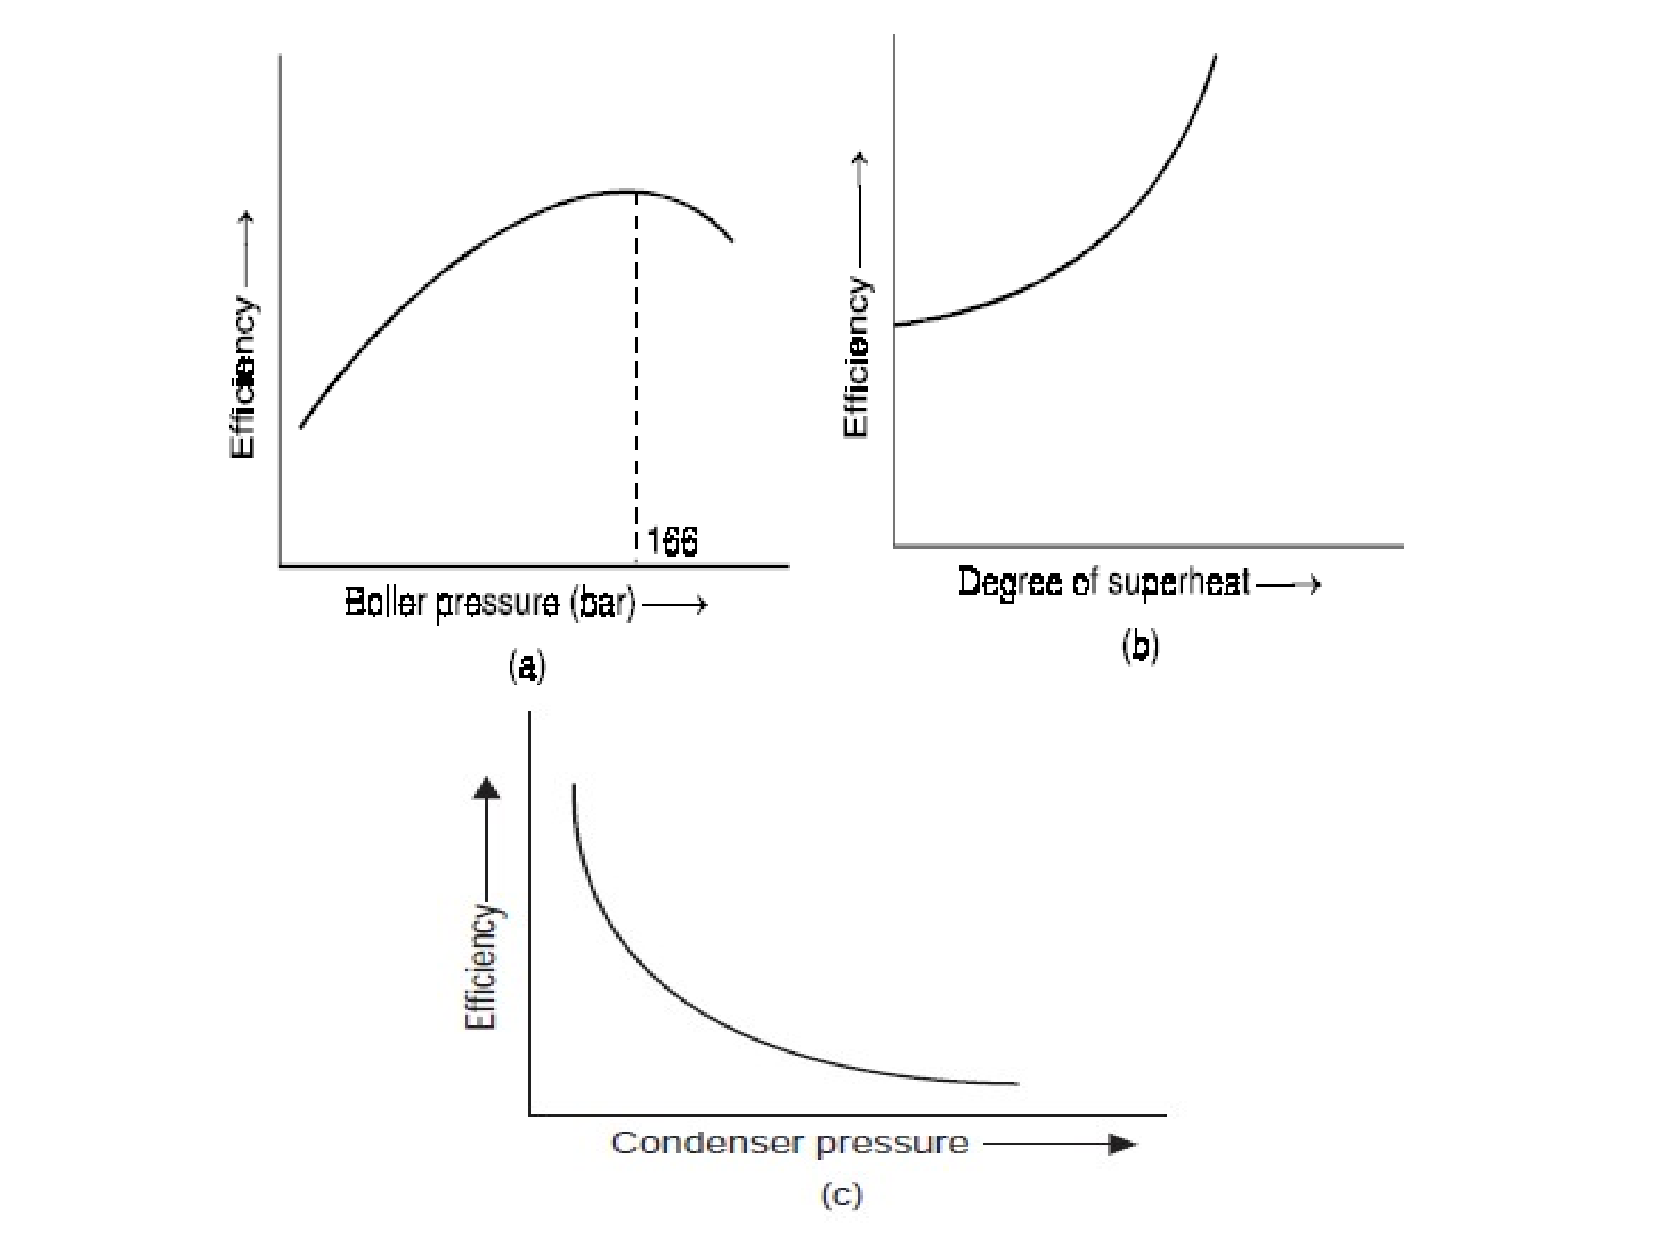
\includegraphics[width=8.cm,clip]{./Pics/Rankine_Improving_Efficiency}
     \end{center}
    \end{figure}
 \normalsize
\end{frame}





%%%
%%% Slide
%%%
\begin{frame}
 \frametitle{Example 1: Simple Steam Power Plant}
 %\scriptsize
    {\it The table below represents the steps of an idealised steam power plant with
    \begin{center}
     \begin{tabular}{||c | c | c | c | c ||}
      \hline\hline
       {\bf Step} & {\bf Location}       & {\bf Pressure}  & {\bf Temperature /}   & {\bf Velocity} \\
                  &                      & {\bf (bar)}     & {\bf Quality}         & {\bf m/s}      \\
      \hline\hline
          1       & Inlet to turbine     &   60            &   380 $^{o}$C          &   --           \\
      \hline
          2       & Exit from turbine and&   0.1           &   0.9                 & 200             \\
                  & inlet to condenser   &                 &    --                 &     --          \\ 
      \hline
          3       & Exit from condenser and&  0.09         &  Saturated            &   --            \\
                  & inlet to pump        &                 &  Liquid               &                 \\
      \hline
          4       & Exit from pump and   &  70             &   --                  &     --          \\
                  & inlet to boiler      &                 &                       &                 \\
      \hline 
          5       & Exit from boiler     &  65             &  400 $^{o}$C           &      --        \\
                  & Rate of steam flow:   &                 &                       &                 \\
                  & 1.0$\times$10$^{4}$ kg/h &             &                       &                 \\
     
      \hline\hline
     \end{tabular}
    \end{center}}
 \normalsize
\end{frame}


%%%
%%% Slide
%%%
\begin{frame}
 \frametitle{Example 1: Simple Steam Power Plant}
 %\scriptsize
    {\it Calculate:
    \begin{enumerate}[(a)]
     \item Power output of the turbine.
     \item Heat transfer per hour in the boiler and condenser.
     \item Mass rate of cooling water circulated (kg/h) in the condenser assuming inlet and outlet fluid temperatures from the condenser of 20$ ^{o}$C and 30 $^{o}$C.
     \item Diameter of the pipe connecting the turbine with the condenser. 
    \end{enumerate}}
 \normalsize
\end{frame}



%%%
%%% Slide
%%%
\begin{frame}
 \frametitle{Example 1: Simple Steam Power Plant}
     
\begin{center}
       \begin{tabular}{|c c c c c|}
         \hline
          P(bar) /   &      &   300       &  350     &  400 \\
          T($^{o}$C) &       &             &         &      \\
          \hline
             60     &  $h$ (kJ/kg)   &   2884.2   & 3043.0   &  3177.2 \\
          \hline
       \end{tabular} 
\end{center}

    \begin{figure}%
     \begin{center}
      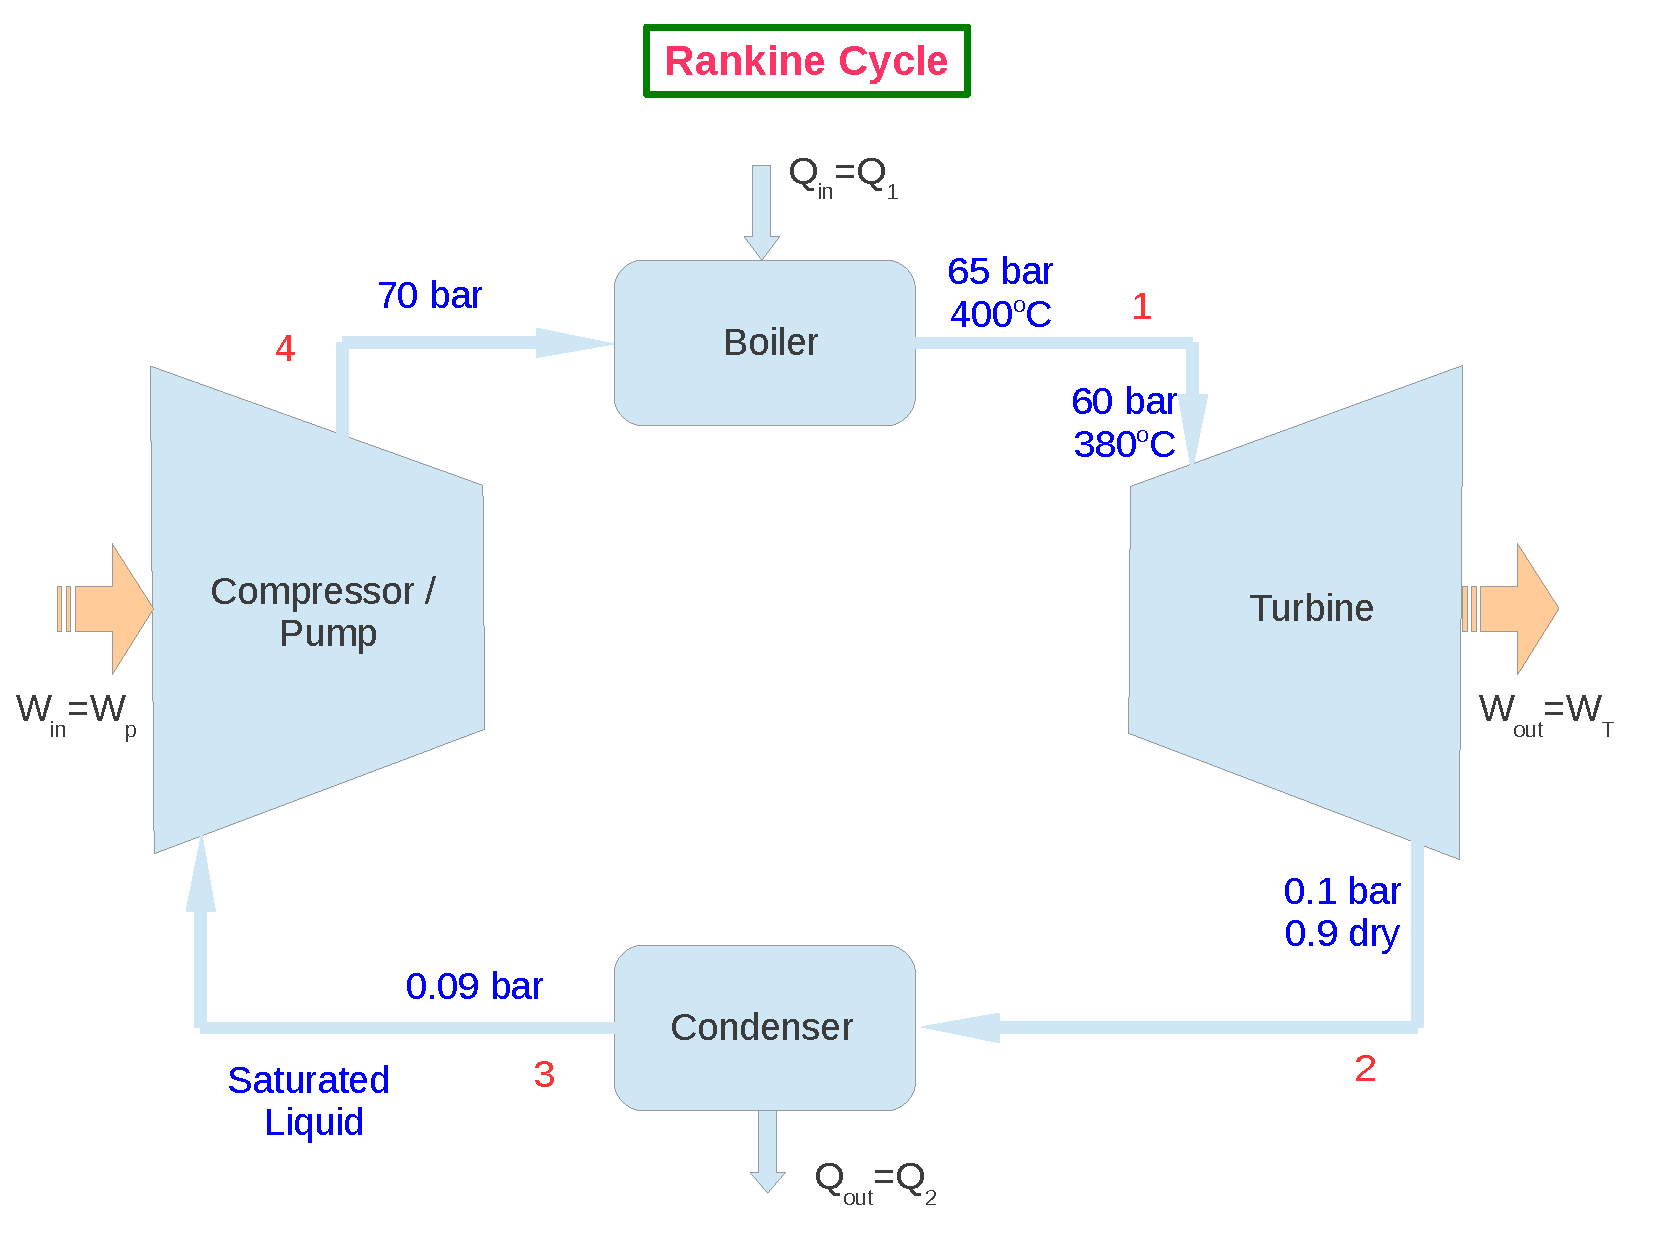
\includegraphics[width=7.5cm,clip]{./Pics/Rankine_Cycle_Exemple01}
     \end{center}
    \end{figure} 


 \normalsize
\end{frame}



%%%
%%% Slide
%%%
\begin{frame}
 \frametitle{Example 1: Simple Steam Power Plant}

    \textcolor{blue}{(a) Power output of the turbine:} From superheated steam table at 60 bar (above), the enthalpy at 380 $^{o}$C is calculated via linear interpolation:\\
        $h_{1}=3043.0 + \displaystyle\frac{3177.2-3043.0}{400-350}\left(380.0-350.0\right)$\\
        $h_{1}=3123.5\;\;kJ/kg$ \\
 
    The pressure at the output from the turbine is 0.1 bar and the enthalpies are:\\
\begin{center}
    \begin{tabular}{|c c c c c|}
     \hline
     P    & T$_{S}$  & h$_{f}$  & h$_{fg}$ & h$_{g}$ \\
    (bar) & ($^{o}$C) & (kJ/kg) & (kJ/kg) & (kJ/kg) \\
    \hline
     0.1 &  45.8     & 191.8   & 2392.8  & 2584.7 \\
    \hline 
    \end{tabular}
\end{center}

    with $x_{2}=0.9$. Thus:\\
    $h_{2}=h_{f_{2}}+x_{2}h_{fg_{2}} = 191.8 + 0.9\times 2392.8$\\
    $h_{2}=2345.3 kJ/kg$\\
    And the power output of the turbine, $P_{T}$ (assuming rate of steam flow on 10000 kg/h:\\
    $P_{T}=m_{s}\left(h_{1}-h_{2}\right)=\displaystyle\frac{1.0\times 10^{4}}{3600}\left(3123.5-2345.3\right)$\\
    \textcolor{blue}{$P_{T}=2162 kW$}

 \normalsize
\end{frame}



%%%
%%% Slide
%%%
\begin{frame}
 \frametitle{Example 1: Simple Steam Power Plant}
 %\scriptsize
    {\it 
    \textcolor{blue}{(b) Heat transfer (per hour) in the boiler $\&$ condenser:} the fluid enters in the boiler at 70 bar $\left(h_{f_{4}}=1267.4\;kJ/kg\right)$ and leaves at 65 bar $\left(T=400^{o}C\right)$ with the enthalpy calculated via linear interpolation of the superheated steam enthalpies at 60 and 70 bars:}\\
\medskip
$h_{\text{out}}^{\text{boiler}}=\displaystyle\frac{3177.2-3158.1}{2}=3167.6\;kJ/kg$\\
The heat transfer in the boiler is, \\
$Q_{1}=m_{s}\left(h_{\text{out}}^{\text{boiler}}-h_{4}\right)=10^{4}\times\left(3167.65-1267.4\right)=1.9\times 10^{7}\;kJ/kg$
\\
\medskip
Now, the heat transfer in the condenser is,\\
\medskip
$Q_{2}=m_{s}\left(h_{2}-h_{3}\right)=10^{4}\times\left(2345.3-183.3\right)=2.16\times 10^{7}\; kJ/h$\\
\medskip

\textcolor{blue}{(c) Mass of cooling water circulated (per hour) in the condenser, $m_{w}$:} The heat lost by the steam is fully transferred to the cooling water,\\
\medskip 
$Q_{2}=m_{w}C_{p,w}\left(T_{2}-T_{1}\right)$\\
\medskip
$2.16\times 10^{7} = m_{w}\times 4.18\left(30-20\right)$\\
\medskip
\textcolor{blue}{$m_{w}=5.17\times 10^{5}\;kg/h$}


 \normalsize
\end{frame}



%%%
%%% Slide
%%%
\begin{frame}
 \frametitle{Example 1: Simple Steam Power Plant}
 %\scriptsize
  \begin{columns}
   \begin{column}[c]{0.5\linewidth}
    {\it  
    \textcolor{blue}{(d) Diameter $\left(\phi\right)$ of the pipe connecting the turbine and the condenser:}\\
$\displaystyle\frac{\pi}{4}\phi^{2}u_{s}=m_{s}x_{2}v_{g_{2}}$\\
where $u_{s}$ and $v_{g_{2}}$ are the steam velocity (=200 m/s) and the specific volume at 0.1 bar $\left(=14.67\;m^{3}/kg\right)$, respectively. Substituting the values in the expression above,\\
\textcolor{blue}{$\phi=0.483\;m$}
}
   \end{column}

   \begin{column}[c]{0.5\linewidth}
    \begin{figure}%
     \begin{center}
      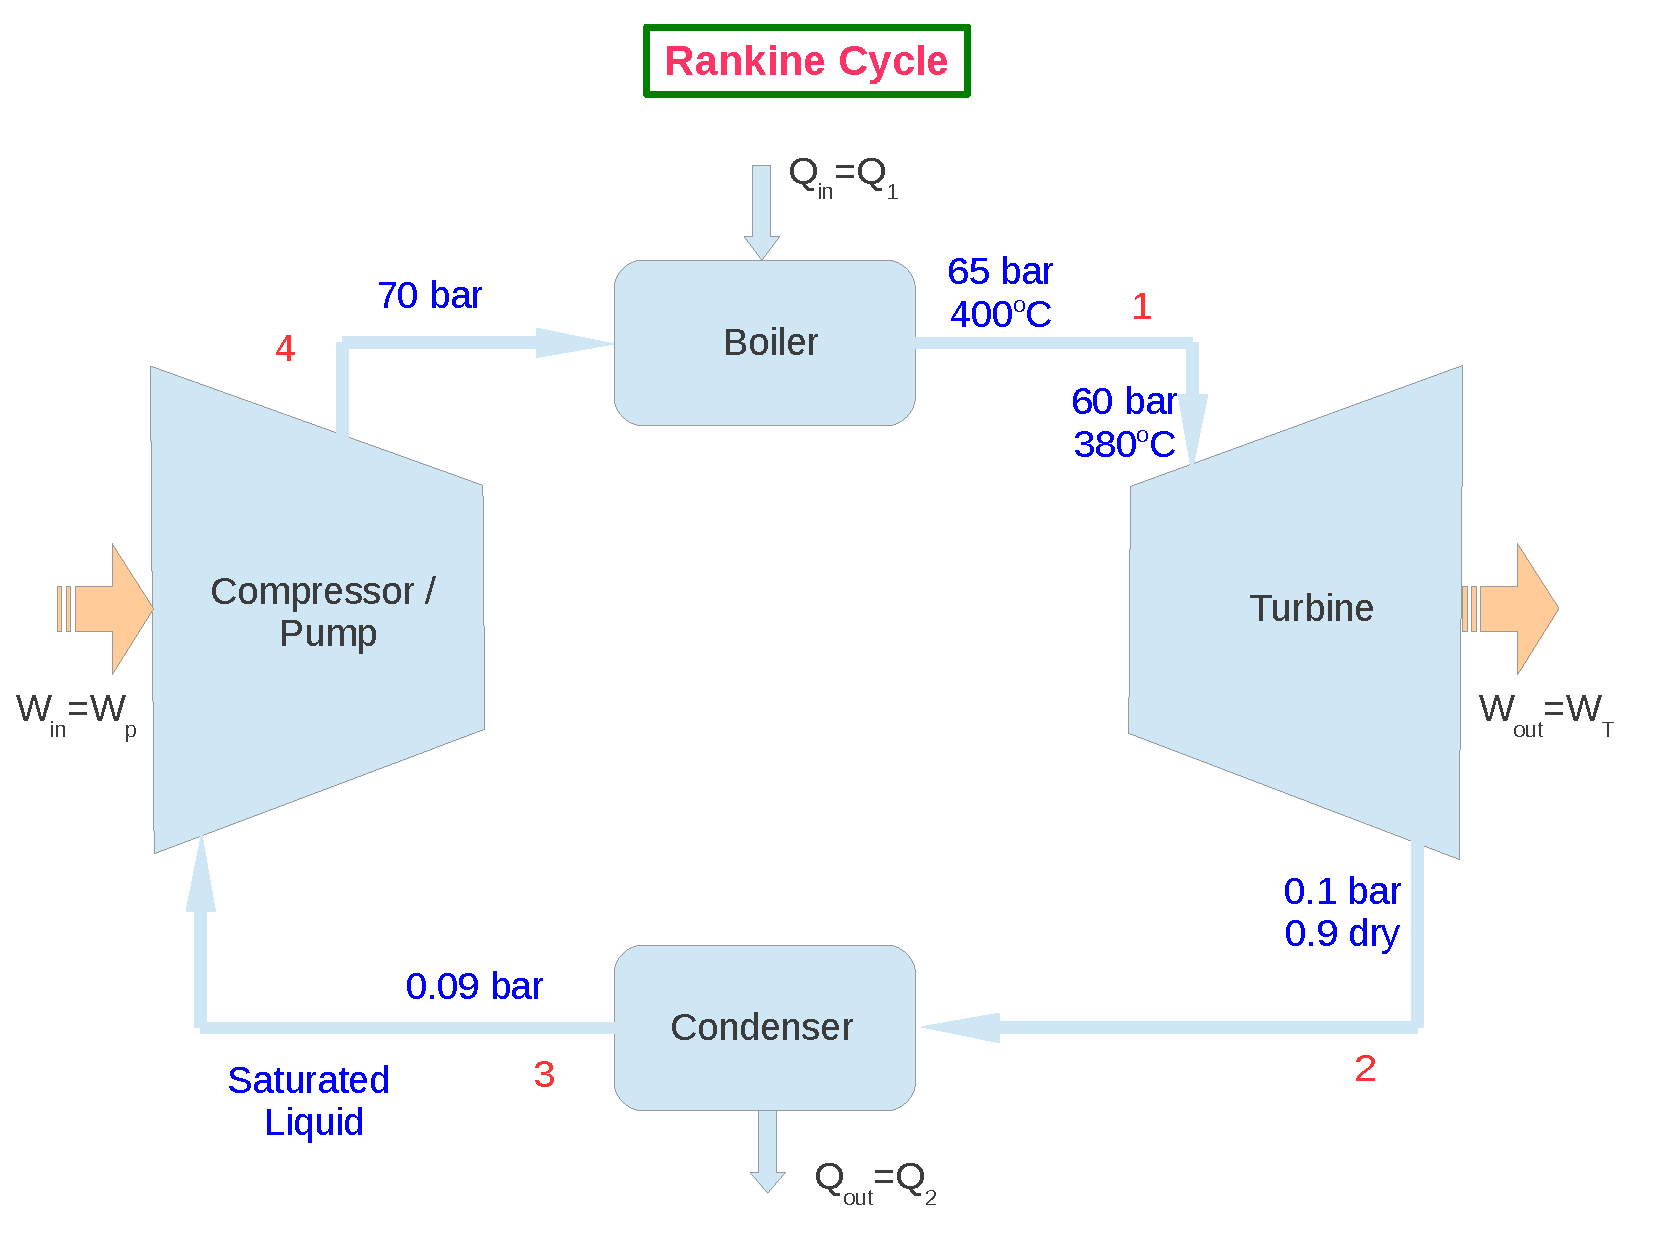
\includegraphics[width=6.25cm,clip]{./Pics/Rankine_Cycle_Exemple01}
     \end{center}
    \end{figure}  
   \end{column}
  \end{columns}

 \normalsize
\end{frame}




%%%
%%% Slide
%%%
\begin{frame}
 \frametitle{Example 2: Carnot and Rankine efficiencies}
 %\scriptsize
Steam (dry and saturated) is supplied by the boiler at 15 bar and the condenser pressure is 0.4 bar. Calculate the Carnot and Rankine efficiencies of the cycle. Neglect the pump work.

\medskip

{\it
\begin{tabular}{c| c c c c}
\hline
 {\bf $P_{1}=15$}  & $x_{1}=1$                & $T_{s}=198.3$  & $h_{g}=2789.9$   & $s_{g}=6.4406$ \\ 
 {\bf $P_{2}=0.4$} & $T_{s}=75.9$             & $h_{f}=317.7$  & $h_{fg}=2319.2$  & $s_{f}=1.0261$  \\
                  &                          &                &                 & $s_{fg}=6.6448$ \\ 
\hline
\end{tabular}\\
with $[P]=\text{bar}$, $[T]=^{o}C$, $[h]=kJ/kg$ and $[s]=kJ/(kg/K)$. The Carnot efficiency is defined as \\
\medskip
$\eta_{\text{Carnot}}=\displaystyle\frac{T_{1}-T_{2}}{T_{1}}= \displaystyle\frac{471.3-348.9}{471.3}\left[\displaystyle\frac{K}{K}\right]\;\Longrightarrow\;$ \textcolor{blue}{$\eta_{\text{Carnot}}=0.259\text{ or }25.9\%$}.\\
\medskip
And the Rankine efficiency is \\
\medskip
 $\eta_{\text{Rankine}}=\displaystyle\frac{\text{Adiabatic or isentropic heat drop}}{\text{Heat supplied}}=\displaystyle\frac{h_{1}-h_{2}}{h_{1}-h_{f_{2}}}$\\
\medskip
where $h_{2}=h_{f_{2}}+x_{2}h_{fg_{2}}=317.7+2319.2x_{2}$. 
}
 \normalsize
\end{frame}


%%%
%%% Slide
%%%
\begin{frame}
 \frametitle{Example 2: Carnot and Rankine efficiencies}
 %\scriptsize

{\it 

\medskip 
We need to calculate the water steam quality, $x_{2}$, and as the steam expands isentropically, i.e., $s_{1}=s_{2}$, therefore,\\
\medskip
$6.4406=s_{f_{2}}+x_{2}s_{fg_{2}}=1.0261+6.6448x_{2}$ $\Longrightarrow$ $x_{2}=0.815$\\
\medskip
The enthalpy at the condenser can then be easily calculated as $h_{2}=317.7+0.815\times 2319.2=2207.8\;kJ/kg$. And the Rankine efficiency is,\\
\medskip
\textcolor{blue}{$\eta_{\text{Rankine}}=0.2354\text{ or }23.54\%$}
}

\normalsize
\end{frame}


\begin{comment}
%%%
%%% Slide
%%%
\begin{frame}
 \frametitle{Example 3: Improving thermal efficiency in Rankine cycles}

\begin{center}
{\Large \textcolor{blue}{See Problem 2.3}}
\end{center}
 %\scriptsize
 \normalsize
\end{frame}
\end{comment}


\subsection{Modified Rankine Cycles}
%%%
%%% Slide
%%%
\begin{frame}
 \frametitle{The Ideal Reheat Rankine Cycle}
  \begin{columns}
   \begin{column}[c]{0.5\linewidth}

 \begin{itemize} %\scriptsize
  \item <1-> Thermal efficiency can be enhanced by increasing the boiler pressure (see Example 3 of Tutorial 2);
  \item <2-> However, this results in higher moisture content in the steam flow which can damage the turbine;
 \end{itemize}
   \end{column}

   \begin{column}[c]{0.5\linewidth} 
    \begin{figure}%
     \begin{center}
      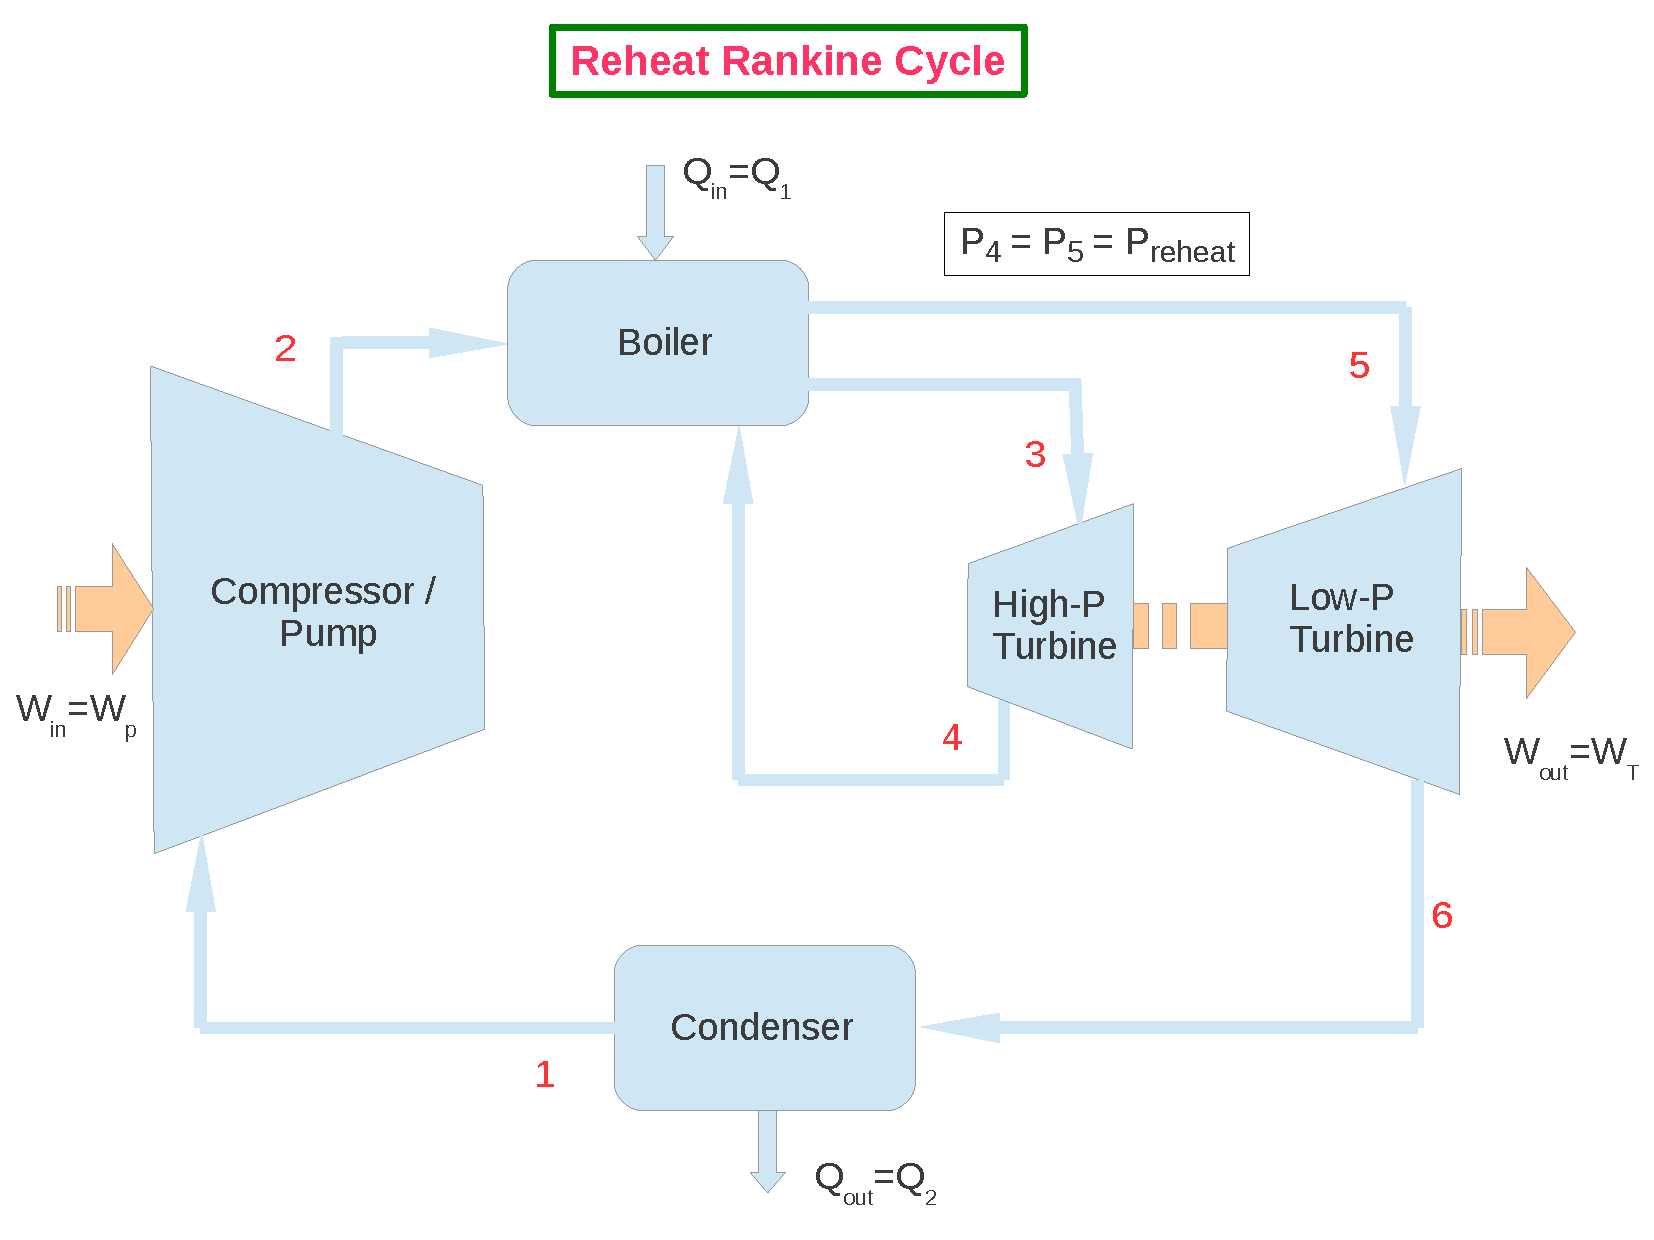
\includegraphics[width=6.25cm,clip]{./Pics/Reheat_Rankine_Cycle}
     \end{center}
    \end{figure}  
   \end{column}
  \end{columns}
 \normalsize
\end{frame}



%%%
%%% Slide
%%%
\begin{frame}
 \frametitle{The Ideal Reheat Rankine Cycle}
  \begin{columns}
   \begin{column}[c]{0.5\linewidth}

 \begin{itemize} %\scriptsize
  \item <1-> To overcome this problem we may:
  \begin{enumerate}[(a)] %\scriptsize
   \item <2-> Superheat the steam before the turbine: this would improve thermal efficiency of the cycle but the very high temperature may be prohibitive as novel (and more expansive) material would need to be used;
   \item <3-> Expand the steam in the turbine in two stages and reheat in between. This is an improvement on the ideal Rankine cycle as we would add a reheating process between continuous expansion.
  \end{enumerate} 
 \end{itemize}
   \end{column}

   \begin{column}[c]{0.5\linewidth} 
    \begin{figure}%
     \begin{center}
      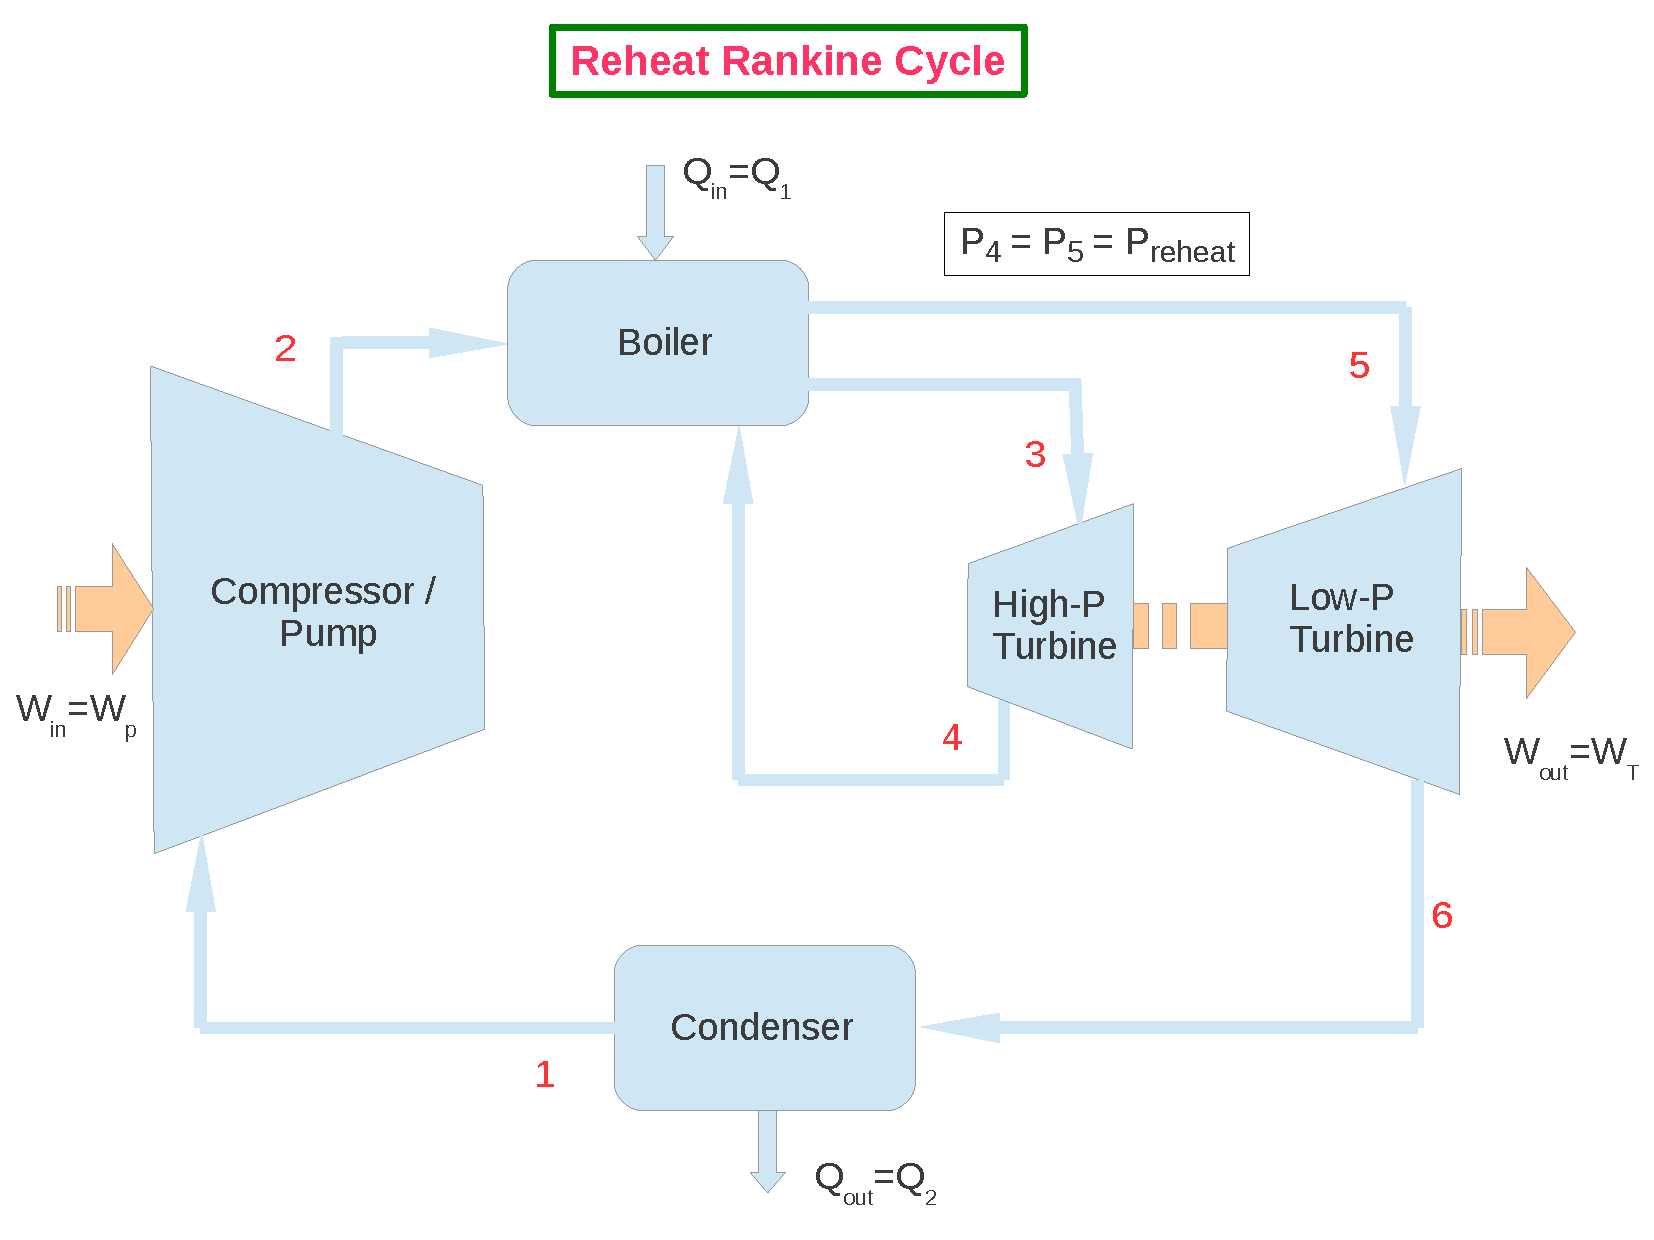
\includegraphics[width=6.25cm,clip]{./Pics/Reheat_Rankine_Cycle}
     \end{center}
    \end{figure}  
   \end{column}
  \end{columns}
 \normalsize
\end{frame}





%%%
%%% Slide
%%%
\begin{frame}
 \frametitle{The Ideal Reheat Rankine Cycle}
  \begin{columns}
   \begin{column}[c]{0.5\linewidth}

 \begin{itemize} %\scriptsize
  \item <1-> Expansion occurs in a 2-stages process:
  \begin{enumerate}[(a)] %\scriptsize
   \item <2-> {\it First Stage (High-P Turbine):} steam is expanded isentropically to an intermediate pressure and return to the boiler where it is reheated at constant pressure;
   \item <3-> {\it Second Stage (Low-P Turbine:} steam is expanded isentropically to the condenser pressure;
  \end{enumerate}
  \item <4-> Total heat input is $q_{\text{in}}=q_{\text{primary}}+q_{\text{reheat}}=$$\left(h_{3}-h_{2}\right)+\left(h_{5}-h_{4}\right)$;
  \item <5-> Total turbine work output is $W_{\text{turb}}^{\text{out}} = W_{\text{turb}}^{\text{high-P}} + W_{\text{turb}}^{\text{low-P}}=$ $\left(h_{3}-h_{4}\right)+\left(h_{5}-h_{6}\right)$
 \end{itemize} 
   \end{column}

   \begin{column}[c]{0.5\linewidth} 
    \begin{figure}%
     \begin{center}
      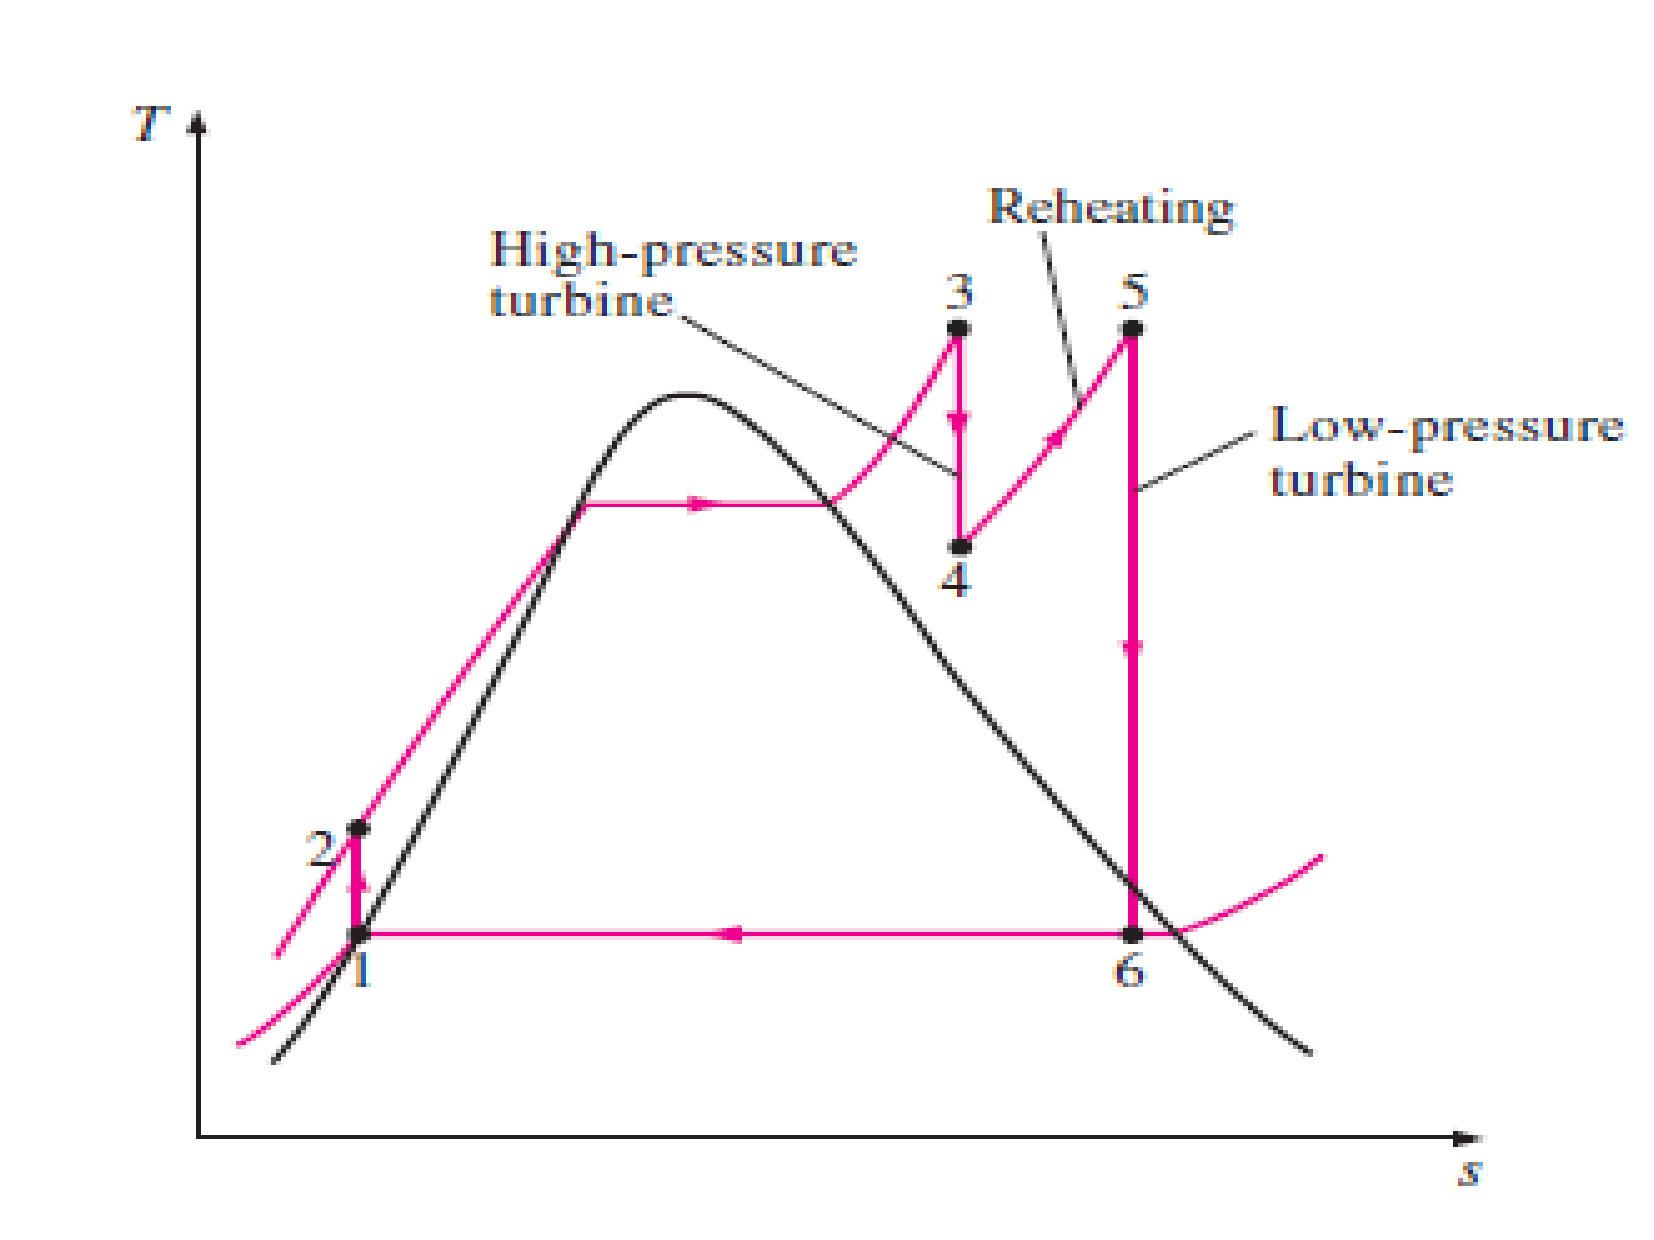
\includegraphics[width=6.25cm,clip]{./Pics/Reheat_Rankine_Cycle_Diagram}
     \end{center}
    \end{figure}  
   \end{column}
  \end{columns}

 %\scriptsize
 \normalsize
\end{frame}



%%%
%%% Slide
%%%
\begin{frame}
 \frametitle{Advantages of Reheat Rankine Cycle}
  \begin{itemize}
   \item <1-> The main objective of using superheated steam is \textcolor{blue}{to avoid excessive moisture in the steam} at the end of the expansion process;
   \item <2-> A large moisture content in the steam would lead to larger condensation in the engine cyclinder, and it would result in blade erosion;
   \item <3-> Maximum moisture content of approx. 12$\%$ to avoid blades' damage;
   \item <4-> Thus superheated steam:
   \begin{enumerate}
    \item <5-> leads a reduction in the initial condensation losses in steam engines;
    \item <6-> improves the plant efficiency by saving fuel (costs).
    \item <7-> Reheating should be operated at \textcolor{blue}{optimum pressure};
    \item <8-> If the steam is reheated nearly in its expansion then the additional heat that need to be supplied will be small and the thermal efficiency gain will be small;
    \item <9-> If the reheating is operated at a fairly low pressure, then, although a large amount of additional heat is supplied, the steam will have a high degree of superheat (Mollier diagram), thus a large proportion of the heat supplied in the reheating process will be wasted in the condenser.
   \end{enumerate}
  \end{itemize}
 
\end{frame}


%%%
%%% Slide
%%%
\begin{frame}
 \frametitle{Advantages of Reheat Rankine Cycle}
 \begin{itemize}
  \item <1->\textcolor{blue}{Advantages of Reheating:}
   \begin{enumerate}
    \item <2-> There is an increased output from the turbine;
    \item <3-> Smaller problems -re to erosion and corrosion;
    \item <4-> Improvement of the thermal efficiency of the turbines;
    \item <5-> Smaller moisture content in the steam flow;
   \end{enumerate}
  \item <6->\textcolor{blue}{Disavantages of Reheating:}
   \begin{enumerate}
    \item <7-> Reheating requires more maintenance;
    \item <8-> Enhancement of thermal efficiency may not be enough to match the larger costs associated with reheating the steam.
   \end{enumerate}
 \end{itemize}
\end{frame}



%%%
%%% Slide
%%%
\begin{frame}
 \frametitle{Ideal Regenerative Rankine Cycle}
  \begin{columns}
   \begin{column}[c]{0.5\linewidth}
    \begin{enumerate} %\scriptsize
     \item <1-> In simple Rankine cycle the temperature of the working fluid entering the boiler is substantially lower than the boiler steam exiting temperature.  This results in lower thermal efficiency;
     \item <2-> In the {\it Regenerative Rankine Cycle} the temperature of the fluid leaving the pump ({\it feedwater}) is raised in several stages using steam extracted from the turbine;
     \item <3-> The device where the feedwater is heated by regeneration is called a {\it regenerator}, or a {\it feedwater heater (FWH)};
     %\item <4-> Not only improve thermal efficiency but also deaerates the feedwater that helps prevent corrosion and pump cavitation;
     %\item <5-> A FWH is a heat exchanger where heat is transferred from the steam to the feedwater either by mixing the two fluid streams ({\it open feedwater heaters}) or without mixing them ({\it closed feedwater heaters}).
    \end{enumerate} 
   \end{column}

   \begin{column}[c]{0.5\linewidth} 
    \begin{figure}%
     \begin{center}
      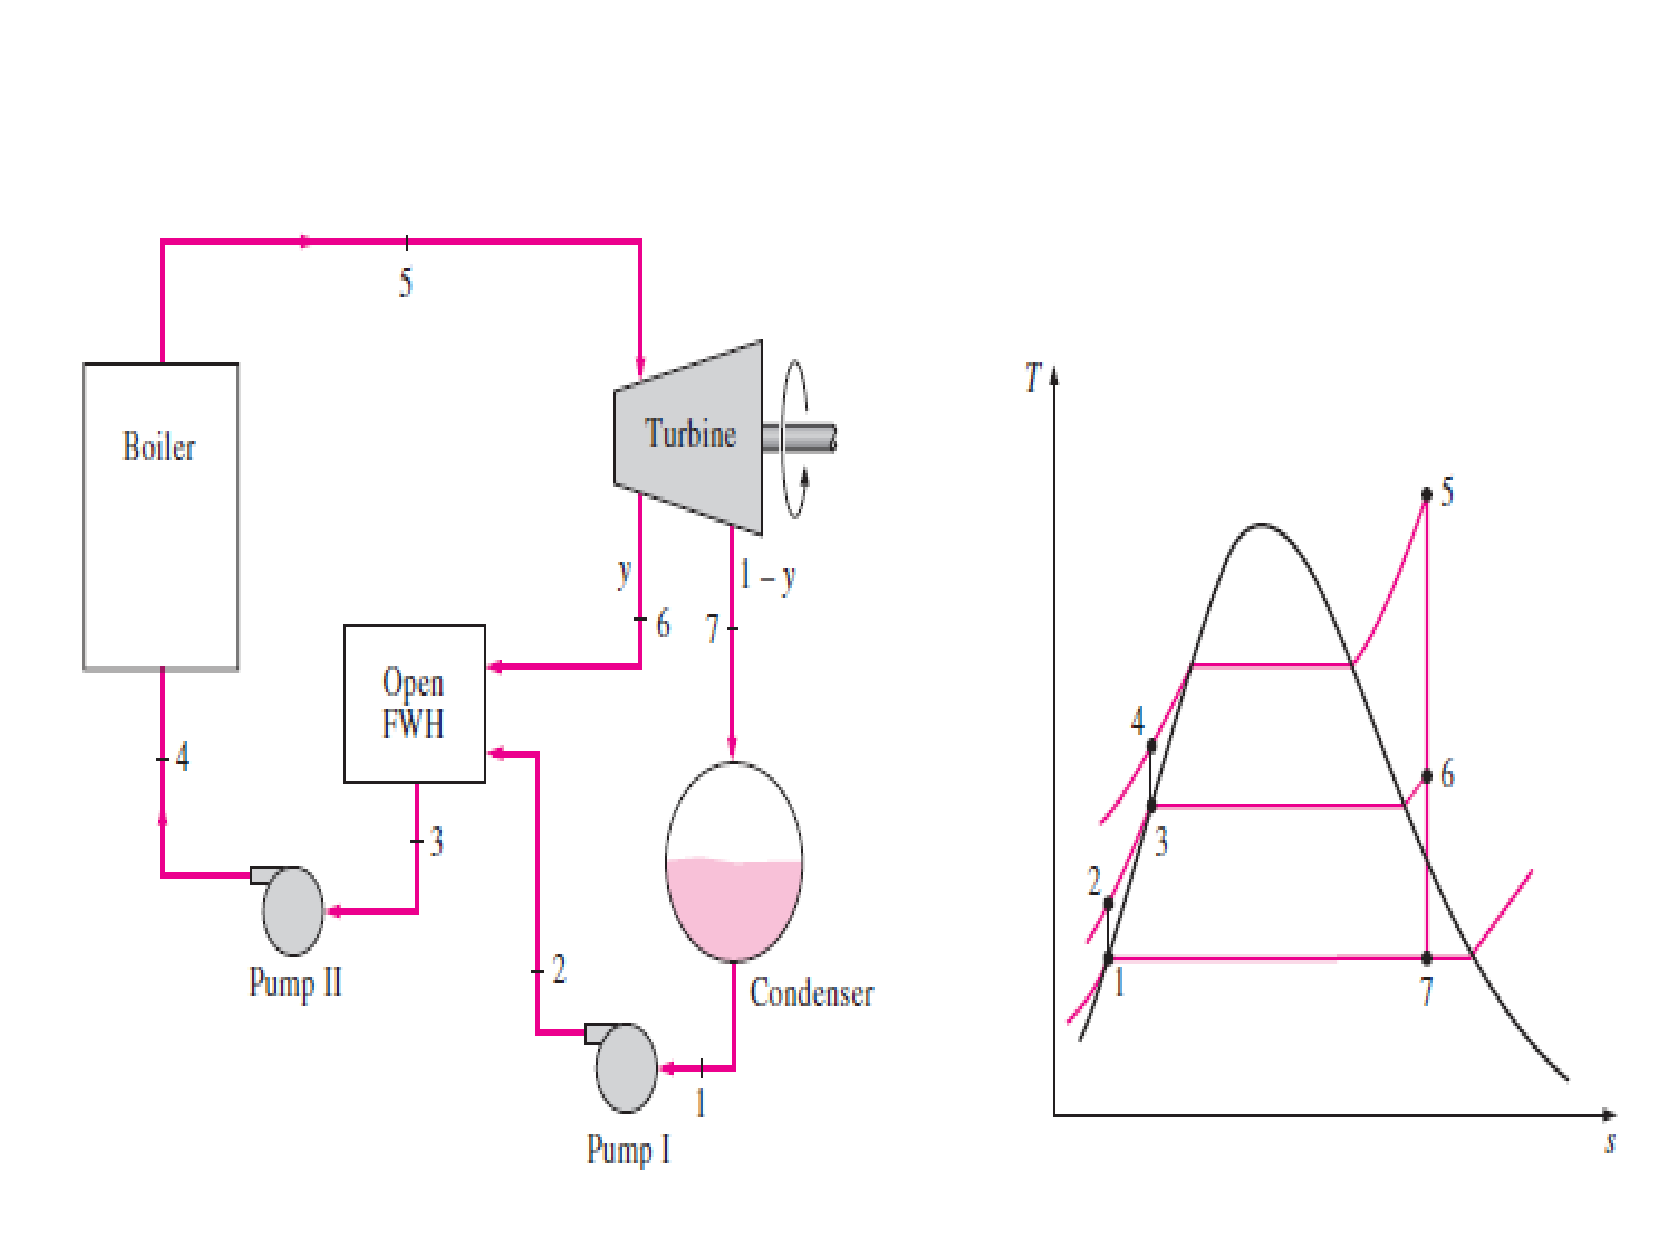
\includegraphics[width=6.25cm,clip]{./Pics/Regenerative_Rankine_Cycle_OpenFWH}
      \caption{\scriptsize Open feedwater heater.} 
     \end{center}
    \end{figure}  
   \end{column}
  \end{columns}
 \normalsize
\end{frame}



%%%
%%% Slide
%%%
\begin{frame}
 \frametitle{Ideal Regenerative Rankine Cycle}
  \begin{columns}
   \begin{column}[c]{0.5\linewidth}
    \begin{enumerate} %\scriptsize
     %\item <1-> In simple Rankine cycle the temperature of the working fluid entering the boiler is substantially lower than the boiler steam exiting temperature.  This results in lower thermal efficiency;
     %\item <2-> In the {\it Regenerative Rankine Cycle} the temperature of the fluid leaving the pump ({\it feedwater}) is raised in several stages using steam extracted from the turbine;
     %\item <3-> The device where the feedwater is heated by regeneration is called a {\it regenerator}, or a {\it feedwater heater (FWH)};
     \item <1-> Not only improve thermal efficiency but also deaerates the feedwater that helps prevent corrosion and pump cavitation;
     \item <2-> A FWH is a heat exchanger where heat is transferred from the steam to the feedwater either by mixing the two fluid streams ({\it open feedwater heaters}) or without mixing them ({\it closed feedwater heaters}).
    \end{enumerate} 
   \end{column}

   \begin{column}[c]{0.5\linewidth} 
    \begin{figure}%
     \begin{center}
      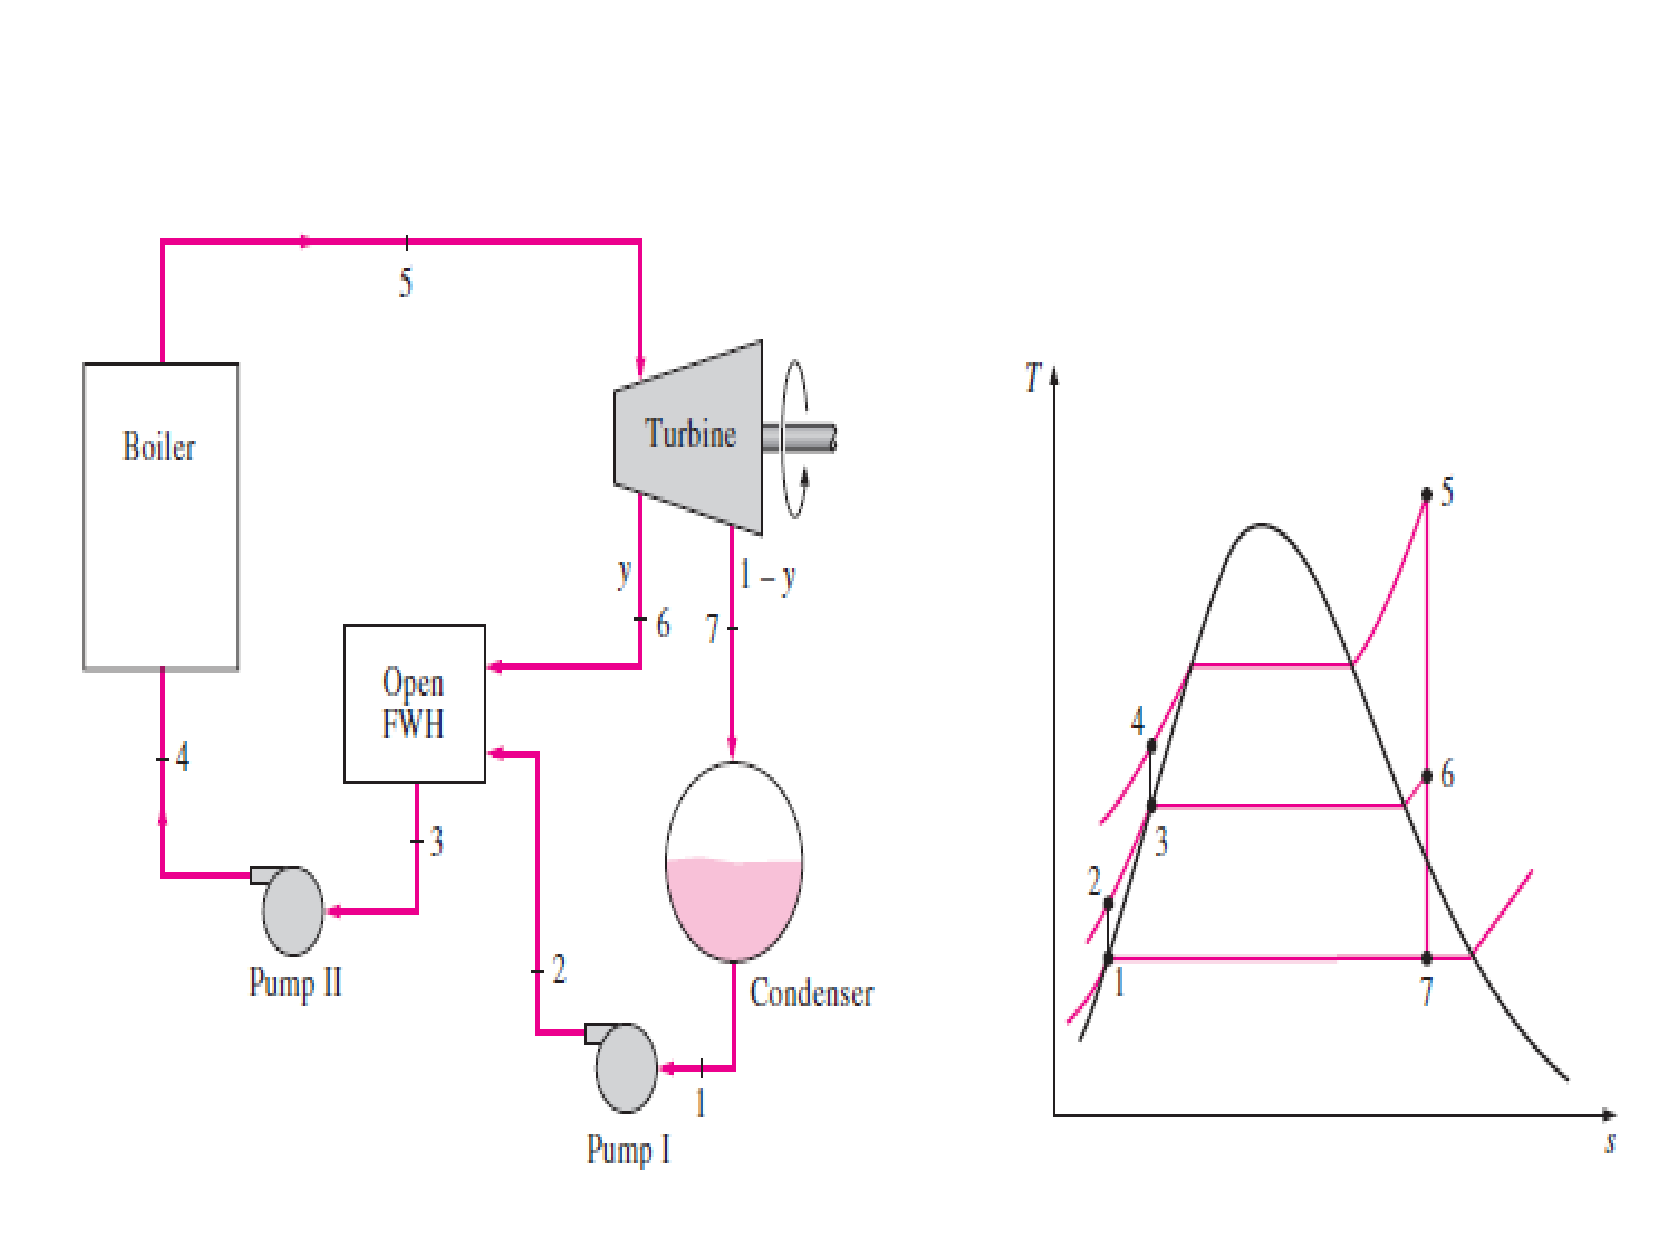
\includegraphics[width=6.25cm,clip]{./Pics/Regenerative_Rankine_Cycle_OpenFWH}
      \caption{\scriptsize Open feedwater heater.} 
     \end{center}
    \end{figure}  
   \end{column}
  \end{columns}
 \normalsize
\end{frame}



%%%
%%% Slide
%%%
\begin{frame}
 \frametitle{Ideal Regenerative Rankine Cycle}

  \begin{columns}
   \begin{column}[c]{0.5\linewidth}
    \begin{enumerate} %\scriptsize
     \item <1-> In Open FWH, steam is expanded isentropically in the turbine from a boiler pressure to an intermediate pressure;
     \item <2-> Part of the steam is then extracted and diverted to the FWH, whereas the remaining steam continues to expand isentropically to the condenser pressure;
      \item <3-> Steam leaves the condenser as a {\it saturated liquid} at the condenser pressure; 
      \item <4-> Feedwater enters the (isentropic) pump and is compressed to the FWH pressure and routed to the FWH where it is mixed with the steam extracted from the turbine;
      %\item <5->  A fraction of the steam extracted from the turbine ($y$) leaves the FWH as a {\it saturated liquid} $\left(P_{\text{FWH}}\right)$, and a second pump raises the pressure to $P_{\text{boiler}}$;
      %\item <6-> Heat added/extracted in the cycle (as shown in Fig.) is \textcolor{blue}{$q_{\text{in}}=h_{5}-h_{4}$} and \textcolor{blue}{$q_{\text{out}}=\left(1-y\right)\left(h_{7}-h_{1}\right)$};
      %\item <7-> Pump and turbine work is \textcolor{blue}{$W_{\text{turb}}^{\text{out}}=\left(h_{5}-h_{6}\right)+\left(1-y\right)\left(h_{6}-h_{7}\right)$} and \textcolor{blue}{$W_{\text{pump}}^{\text{in}}=\left(1-y\right)W_{\text{pump,1}}^{\text{in}}+W_{\text{pump,2}}^{\text{in}}$}
    \end{enumerate} 
   \end{column}

   \begin{column}[c]{0.5\linewidth} 
     \begin{figure}%
     \begin{center}
      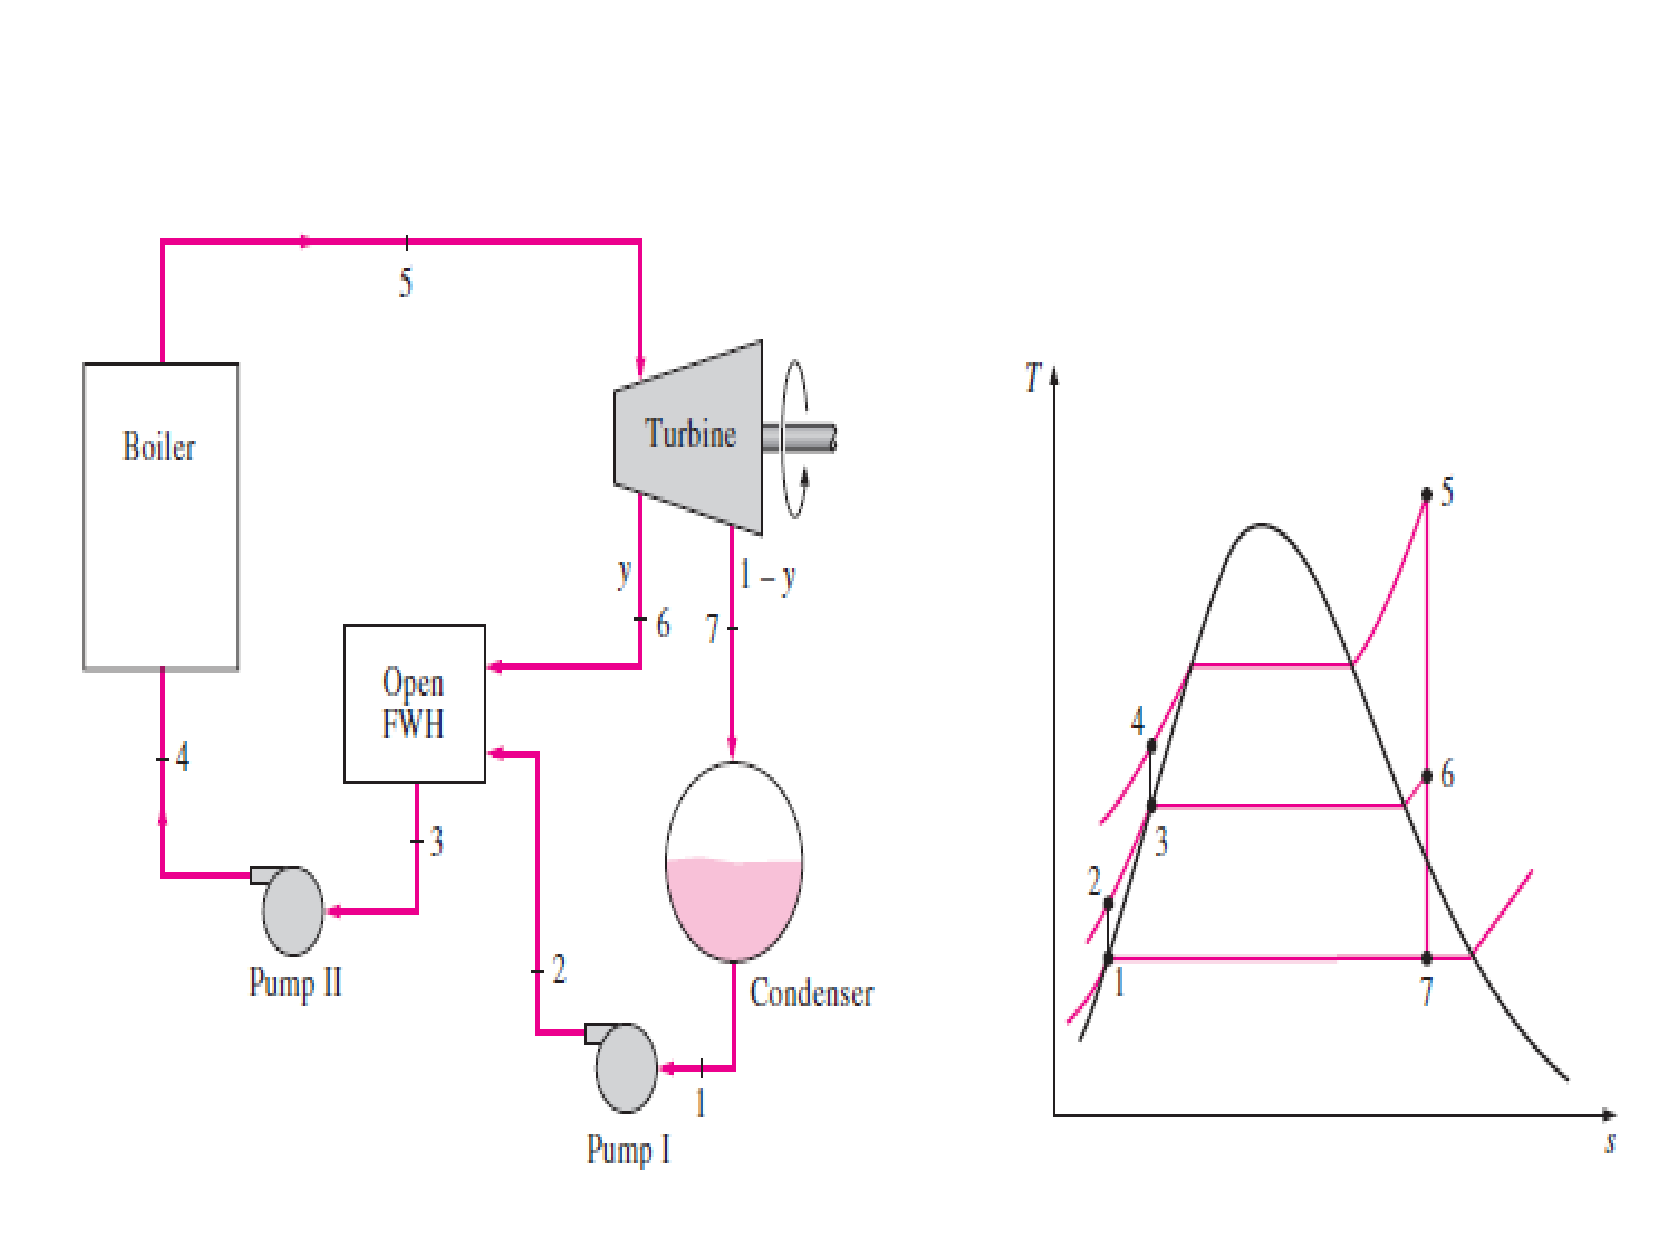
\includegraphics[width=6.25cm,clip]{./Pics/Regenerative_Rankine_Cycle_OpenFWH}
      \caption{\scriptsize Open feedwater heater.} 
     \end{center}
    \end{figure}  
   \end{column}
  \end{columns}
 \normalsize
\end{frame}



%%%
%%% Slide
%%%
\begin{frame}
 \frametitle{Ideal Regenerative Rankine Cycle}

  \begin{columns}
   \begin{column}[c]{0.5\linewidth}
    \begin{enumerate} %\scriptsize
     %\item %<1-> In Open FWH, steam is expanded isentropically in the turbine from a boiler pressure to an intermediate pressure;
     %\item %<2-> Part of the steam is then extracted and diverted to the FWH, whereas the remaining steam continues to expand isentropically to the condenser pressure;
     % \item %<3-> Steam leaves the condenser as a {\it saturated liquid} at the condenser pressure; 
     % \item %<4-> Feedwater enters the (isentropic) pump and is compressed to the FWH pressure and routed to the FWH where it is mixed with the steam extracted from the turbine;
      \item <1->  A fraction of the steam extracted from the turbine ($y$) leaves the FWH as a {\it saturated liquid} $\left(P_{\text{FWH}}\right)$, and a second pump raises the pressure to $P_{\text{boiler}}$;
      \item <2-> Heat added/extracted in the cycle (as shown in Fig.) is \textcolor{blue}{$q_{\text{in}}=h_{5}-h_{4}$} and \textcolor{blue}{$q_{\text{out}}=\left(1-y\right)\left(h_{7}-h_{1}\right)$};
      \item <3-> Pump and turbine work are \\
\medskip
       \textcolor{blue}{$W_{\text{turb}}^{\text{out}}=\left(h_{5}-h_{6}\right)+\left(1-y\right)\left(h_{6}-h_{7}\right)$}  and \\
\medskip
       \textcolor{blue}{$W_{\text{pump}}^{\text{in}}=\left(1-y\right)W_{\text{pump,1}}^{\text{in}}+W_{\text{pump,2}}^{\text{in}}$}
    \end{enumerate} 
   \end{column}

   \begin{column}[c]{0.5\linewidth} 
     \begin{figure}%
     \begin{center}
      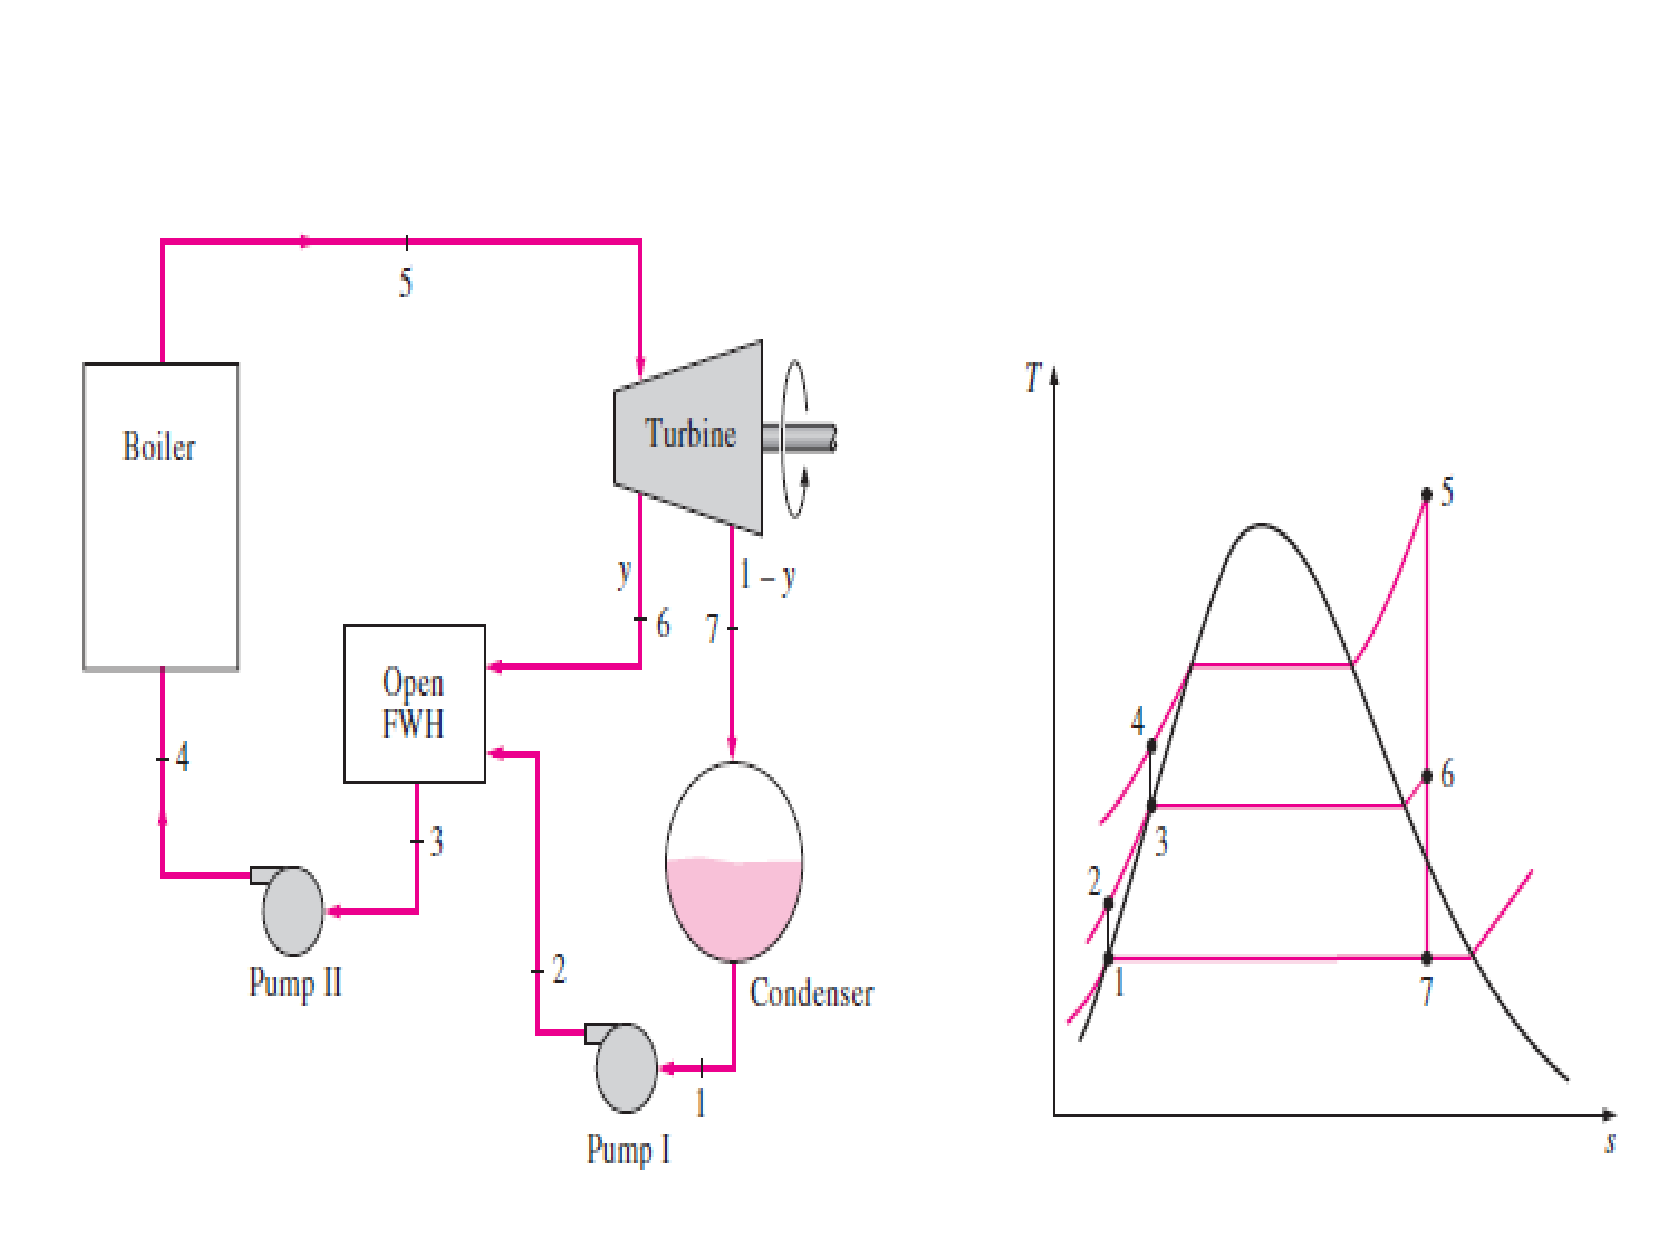
\includegraphics[width=6.25cm,clip]{./Pics/Regenerative_Rankine_Cycle_OpenFWH}
      \caption{\scriptsize Open feedwater heater.} 
     \end{center}
    \end{figure}  
   \end{column}
  \end{columns}
 \normalsize
\end{frame}



%%%
%%% Slide
%%%
\begin{frame}
 \frametitle{Ideal Regenerative Rankine Cycle}
    \begin{figure}%
     \begin{center}
      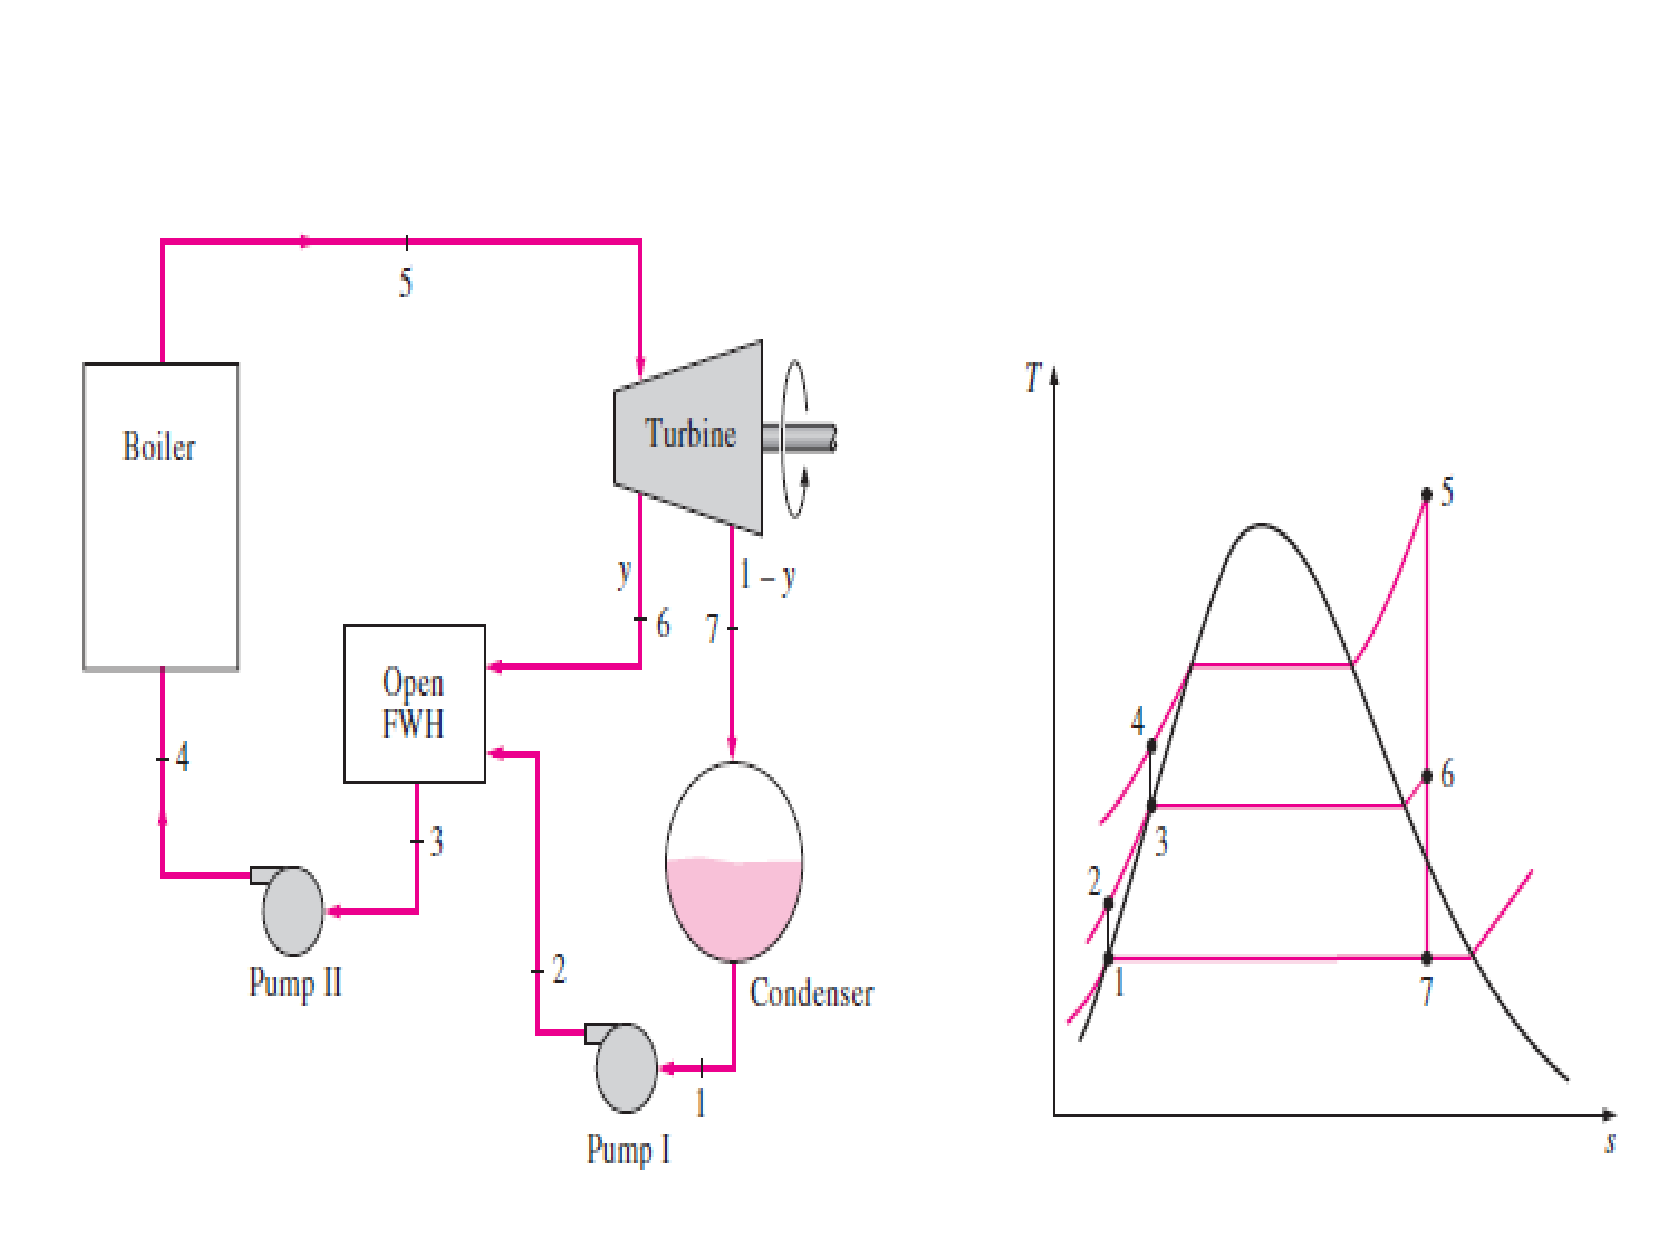
\includegraphics[width=6.25cm,clip]{./Pics/Regenerative_Rankine_Cycle_OpenFWH}
      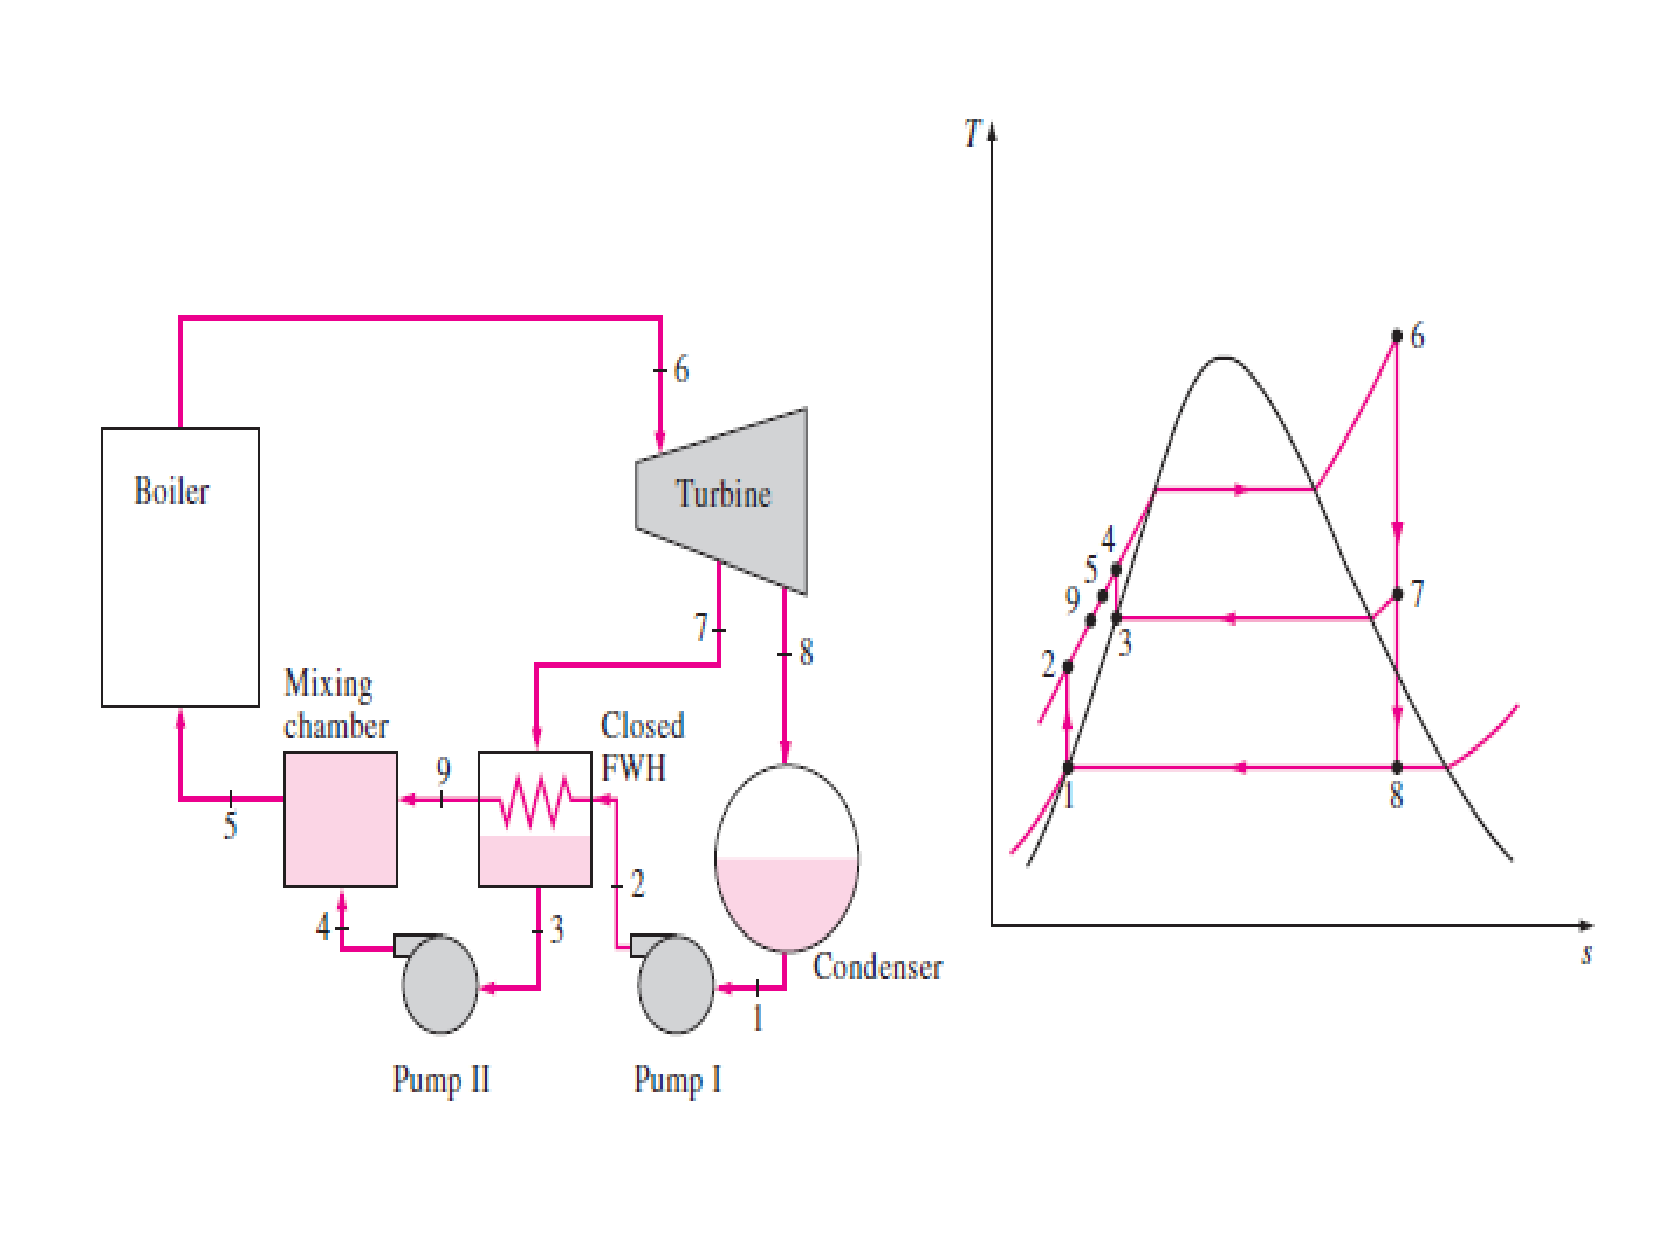
\includegraphics[width=6.25cm,clip]{./Pics/Regenerative_Rankine_Cycle_ClosedFWH}
\caption{Open and closed (rhs) Feedwater Heaters.}
     \end{center}
    \end{figure}  
\end{frame}


%%%
%%% Slide
%%%
\begin{frame}
 \frametitle{Ideal Regenerative Rankine Cycle}
  \begin{columns}
   \begin{column}[c]{0.5\linewidth}
    \begin{itemize}
     \item <1-> Advantages of Regenerative cycle over Simple Rankine Cycle
     \begin{enumerate} %\scriptsize
      \item <2-> The heating process in the boiler tends to become reversible;
      \item <3-> Thermal stresses in boiler are minimised due to the smaller temperature ranges in the boiler;
      \item <4-> Thermal efficiency is improved as the average temperature of heat addition to the cycle is increased;
      \item <5-> Due to continuous steam extraction, the content of moisture is reduced and this decreases the corrosion in the turbine;
      \item<6-> The size of the condenser is smaller (lower cost and better maintenance).
     \end{enumerate}
    \end{itemize} 
   \end{column}

   \begin{column}[c]{0.5\linewidth}  
    \begin{itemize}
     \item <7-> Disadvantages of Regenerative cycle over Simple Rankine Cycle
     \begin{enumerate} %\scriptsize
      \item <8-> Design of the power plant is more complex;
      \item <9-> As the number of heaters is increased, the greater maintenance (larger cost) is required;
      \item <10-> Heater are usually costly and the gain in thermal efficiency may not be enough. 
     \end{enumerate}
    \end{itemize} 
   \end{column}
  \end{columns}
  
\end{frame}



\subsection{Summary}
%%%
%%% Slide
%%%
\begin{frame}
 \frametitle{Summary}
  \begin{itemize}
   \item <1-> Components of vapour power cycles;
   \item <2-> Carnot cycle -- maximum possible efficiency derived from the Second Law of Thermodynamics;
   \item <3-> Rankine cycle is currently used in a number of industrial applications to transform thermal to mechanical/electrical energy;
   \item <4-> Practical improvements to the Rankine cycle to enhance thermal effciency.

  \end{itemize}
\end{frame}


%%%
%%% Slide
%%%
%\begin{frame}
% \frametitle{}
 %\scriptsize
% \normalsize
%\end{frame}







\end{document}
